\documentclass[aps,prd,twocolumn,superscriptaddress,nofootinbib,longbibliography,floatfix,amsmath,amssymb,10pt]{revtex4-2}
\usepackage[utf8]{inputenc}
\usepackage[T1]{fontenc}
\usepackage{amsthm}
\usepackage{mathrsfs}
\usepackage{graphicx}
\usepackage{booktabs}
\usepackage{multirow}
\usepackage{array}
\usepackage{tikz}
\usetikzlibrary{arrows.meta,positioning,calc,matrix,shapes.geometric,decorations.pathreplacing}
\usepackage{xcolor}
\usepackage{enumitem}
\usepackage[colorlinks=true,linkcolor=blue!50!black,citecolor=blue!50!black,urlcolor=blue!50!black]{hyperref}
\usepackage{orcidlink}
\usepackage[protrusion=true,expansion=false]{microtype}
\usepackage{xurl}

\theoremstyle{plain}
\newtheorem{theorem}{Theorem}[section]
\newtheorem{proposition}[theorem]{Proposition}
\newtheorem{lemma}[theorem]{Lemma}
\newtheorem{corollary}[theorem]{Corollary}
\theoremstyle{definition}
\newtheorem{definition}[theorem]{Definition}
\newtheorem{remark}[theorem]{Remark}
\newtheorem{setup}[theorem]{Setting}

\newcommand{\QQ}{\mathbb{Q}}
\newcommand{\ZZ}{\mathbb{Z}}
\newcommand{\RR}{\mathbb{R}}
\newcommand{\CC}{\mathbb{C}}
\newcommand{\PP}{\mathbb{P}}
\newcommand{\Hdg}{\mathrm{Hdg}}
\newcommand{\Hg}{\mathrm{Hg}}
\newcommand{\NS}{\mathrm{NS}}
\newcommand{\Ab}{\mathrm{Ab}}
\newcommand{\Ext}{\mathrm{Ext}}
\newcommand{\Hom}{\mathrm{Hom}}
\newcommand{\End}{\mathrm{End}}
\newcommand{\ch}{\mathrm{ch}}
\newcommand{\Tr}{\mathrm{Tr}}
\newcommand{\trd}{\mathrm{trd}}
\newcommand{\nrd}{\mathrm{nrd}}
\newcommand{\Sp}{\mathrm{Sp}}
\newcommand{\SO}{\mathrm{SO}}
\newcommand{\SU}{\mathrm{SU}}
\newcommand{\SL}{\mathrm{SL}}
\tolerance=2000
\emergencystretch=2em
\hbadness=2000
\hfuzz=1pt
\newcommand{\Alg}{\mathrm{Alg}}
\newcommand{\cD}{\mathcal{D}}
\newcommand{\cA}{\mathcal{A}}
\newcommand{\cS}{\mathcal{S}}
\newcommand{\HC}{\mathbf{HC}}
\newcommand{\AB}{\mathbf{AB}}
\newcommand{\Fii}{\textup{(F2)}}
\newcommand{\Fiii}{\textup{(F3$'$)}}
\newcommand{\zenodoCodeID}{10.5281/zenodo.XXXXXXXX}
\newcommand{\leancount}{four hundred and nine}

\begin{document}

\title{Algebraic Loci of Hodge Classes and the Two Statements Left on Abelian Varieties}

\author{Deep Bhattacharjee\,\orcidlink{0000-0003-0466-750X}}
\email{itsdeep@live.com}
\thanks{$*$\,Corresponding author. Second address: \mbox{d.bhattacharjee@erl-forschung.de}.}
\affiliation{Formerly, Electro-Gravitational Space Propulsion Laboratory (EGSPL), Bhubaneswar, Odisha 751030, India}

\author{Ushashi Bhattacharya\,\orcidlink{0009-0002-2254-3914}}
\email{rai.bhattacharya.in@gmail.com}
\affiliation{Formerly, National Taiwan University, Taipei 106319, Taiwan}

\date{October 17, 2026}

\begin{abstract}
The Hodge conjecture is equivalent to two statements about abelian varieties. We prove this, and we prove that for each statement the set of varieties on which it is known is dense in every family and is either the whole family or a meagre set. We then build the first object each statement needs: a chain of quotients that makes the real multiplication by $\sqrt6$ on K3 surfaces algebraic, a complex on a product of two Weil fourfolds with the Chern character the semiregularity criterion asks for, and a single class on an abelian fourteenfold that carries the exceptional classes of a Mumford fourfold. Neither statement is proved. We say at which step each construction stops.
\end{abstract}

\keywords{Hodge conjecture; abelian varieties; Weil classes; K3 surfaces; semiregularity}

\maketitle

\section{Introduction}\label{sec:intro}

The Hodge conjecture asks that every rational cohomology class of type $(p,p)$ on a smooth complex projective variety be a rational combination of classes of algebraic subvarieties.\footnote{An earlier preprint of the authors, \emph{Relative secant cycles and Hodge classes}, Preprints.org (2026), \nolinkurl{doi:10.20944/preprints202602.0462.v5} \cite{BB26}, claimed a proof of the Hodge conjecture that does not hold, and the present paper replaces it. The secant variety $\mathrm{Sec}^{n}(A^{\vee})$ contains $A^{\vee}$, so the cycle $\Sigma\cap A^{\vee}$ of its Definition~3 is $A^{\vee}$ itself, whose Fourier--Mukai transform is a skyscraper sheaf with no component in degree $2n$, contrary to its Lemma~4. The Weil classes span a $2$-dimensional space on which $K^{\times}$ acts by $\tau\mapsto\tau^{2n}$, while $\eta^{n}$ has character $N(\tau)^{n}$, contrary to its Propositions~1 and~2. Its general case (Theorem~12) applies the Kuga--Satake construction outside Hodge structures of K3 type and assumes the Kuga--Satake correspondence algebraic, which is open. Section~\ref{sec:earlier} lists every point at which that preprint fails.} Hodge raised it in 1950 \cite{Hod50}; Lefschetz had proved it for divisors \cite{Lef24}. It is known in a scattered family of cases and open in general. This paper does three things. It proves that the conjecture is equivalent to two statements about abelian varieties. It proves that the locus on which either statement is known has the same shape in every family, dense and either everything or meagre, so that each statement asks that algebraicity propagate from a dense set of special points to the whole family. And it builds, at the first class each statement has to reach, an explicit object, proves what that object does, and names the step at which it stops. The conjecture does not close here. What the paper adds is a complete account of where the two remaining statements live, two new theorems on real multiplication, by $\QQ(\sqrt6)$ on K3 surfaces and by the cyclic cubic fields $\QQ(\zeta_{7})^{+}$ and $\QQ(\zeta_{9})^{+}$ on the surfaces of Mumford type, the second of which closes the first two cases of the frontier of \cite{BMB26}, and three constructions carried to the point where the next step is a single stated question. Figure~\ref{fig:roadmap} draws this plan.

\begin{figure*}[t]
\centering
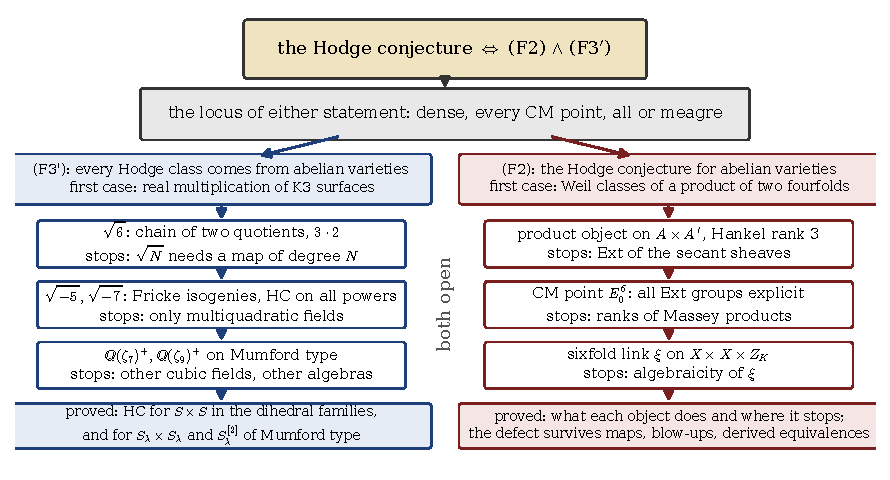
\includegraphics[width=0.96\textwidth]{figures/fig_roadmap}
\caption{The plan of the paper. The conjecture is equivalent to \Fii{} and \Fiii{} (Theorem~\ref{thm:intro-reduction}, Proposition~\ref{prop:minimal}); the locus of either statement is dense, contains every CM point and is all or meagre (Section~\ref{sec:loci}). For \Fiii{} the first class is the real multiplication of K3 surfaces: the chain of quotients for $\sqrt6$ (Theorem~\ref{thm:sqrt6}), the Fricke isogenies for $\sqrt5$ and $\sqrt7$ (Theorem~\ref{thm:fricke}), the cyclic cubic fields on the surfaces of Mumford type (Theorem~\ref{thm:zeta9}), and the steps at which each stops (Propositions~\ref{prop:structure} and~\ref{prop:cubicstop}). For \Fii{} the first class is the Weil classes of a product of two fourfolds: the product object (Theorem~\ref{thm:product}, stopping at Proposition~\ref{prop:convolution}), the point of complex multiplication (Lemma~\ref{lem:cmext}, stopping at Proposition~\ref{prop:twostep}) and the sixfold link (Theorem~\ref{thm:link}, stopping at Section~\ref{ssec:f2stop2}); the defect survives the operations of Proposition~\ref{prop:surgery}.}
\label{fig:roadmap}
\end{figure*}

\subsection{The two statements}

Write $\HC$ for the Hodge conjecture for all smooth complex projective varieties and $\AB$ for its restriction to abelian varieties. For a smooth projective variety $X$ and an integer $p$ let $\Hdg^{p}(X)$ be the Hodge classes of degree $2p$, and let $\Ab^{p}(X)\subseteq\Hdg^{p}(X)$ be the span of the classes $\Gamma_{*}\gamma$, where $B$ runs over the complex abelian varieties (the point included), $\gamma$ over the Hodge classes on $B$, and $\Gamma$ over the algebraic correspondences from $B$ to $X$. The two statements are
\begin{itemize}[leftmargin=2.4em,itemsep=2pt]
\item[\Fii] every Hodge class on every complex abelian variety is algebraic, in the form in which it first appears in the closure computation of \cite{BMB26}: the Hodge classes of the smallest known instance, the exceptional classes on the square of a Mumford fourfold, are algebraic together with everything that can be built from them;
\item[\Fiii] $\Hdg^{p}(X)=\Ab^{p}(X)$ for every $X$ and every $p$: every Hodge class is algebraic modulo the images, under algebraic correspondences, of Hodge classes of abelian varieties.
\end{itemize}

\begin{theorem}[Reduction]\label{thm:intro-reduction}
$\HC$ holds if and only if \Fii{} and \Fiii{} both hold; \Fii{} is equivalent to $\AB$, and \Fiii{} holds on every abelian variety, on every variety dominated by a product of curves or by an abelian variety, and on every variety in degrees $2p$ with $p\in\{0,1,\dim X-1,\dim X\}$.
\end{theorem}

The content of the theorem is in the second sentence: \Fii{} is not a special case of the conjecture for abelian varieties but the whole of it, carried by its hardest classes, and \Fiii{} is exactly what the conjecture asks of the part of the cohomology of $X$ that no abelian variety reaches. Section~\ref{sec:reduction} proves it and places the two statements in the closure graph of the known reductions, with the Lefschetz standard conjecture, Andr\'e's motivated classes and the variational Hodge conjecture as the other nodes (Fig.~\ref{fig:graph}).

\subsection{The shape of the known locus}

For a smooth projective family $\pi\colon\mathcal{X}\to S$ and a flat Hodge class $\xi$ let $\Sigma(\xi)\subseteq S$ be the set of points at which $\xi$ is algebraic.

\begin{theorem}[Dichotomy and propagation]\label{thm:intro-loci}
\leavevmode
\begin{enumerate}[label=\textup{(\roman*)},leftmargin=2.4em,itemsep=2pt]
\item $\Sigma(\xi)$ is a countable union of Zariski closed subsets of $S$, and either $\Sigma(\xi)=S$ or $\Sigma(\xi)$ is meagre.
\item \Fii{} holds if and only if, for every polarised abelian scheme and every flat Hodge class $\xi$, algebraicity of $\xi$ at one point of complex multiplication forces $\Sigma(\xi)=S$.
\item For the Weil classes of every CM field, every $n\ge2$ and every discriminant, $\Sigma(\xi)$ contains an explicit point of complex multiplication and is dense.
\item \Fiii{} holds for $X$ in degree $2p$ if and only if a Hodge complement of the abelian part of $H^{2p}(X,\QQ)$ carries no nonzero Hodge class.
\end{enumerate}
\end{theorem}

So both statements have the same form. There is a dense set of points, the points of complex multiplication, at which the class is known to be algebraic by explicit cycles; the locus of algebraicity is a countable union of closed strata; and the conjecture is the statement that this union is not meagre. Figure~\ref{fig:locus} draws it. Section~\ref{sec:loci} proves the theorem, after \cite{BMB26}, whose argument we rewrite in the generality needed here.

\subsection{Constructions at the first class}

The rest of the paper is constructive. At each statement we go to the first class that is not known and build the object that would make it algebraic.

At \Fiii{} the first class lives on powers of a K3 surface $S$ with real multiplication: the transcendental lattice $T(S)_{\QQ}$ is a vector space over a totally real field $E=\End_{\Hdg}T(S)_{\QQ}$, and the elements of $E$ are Hodge classes on $S\times S$. Section~\ref{sec:f3prime} proves:

\begin{theorem}[Chains of symplectic quotients]\label{thm:intro-chain}
Let $S$ be a projective K3 surface and $e\in E$ with $e^{2}=n\in\QQ_{>0}$. If there is a chain of projective K3 surfaces $S=S_{0},S_{1},\dots,S_{r}$ joined by dominant rational maps or rational Hodge isometries whose degrees multiply to $n$ modulo squares, then $e$ is algebraic on $S\times S$. In particular, for every projective K3 surface $S$ with $\QQ(\sqrt6)\subseteq E$ whose transcendental space embeds in the invariant lattice of a symplectic automorphism of order three, the real multiplication by $\sqrt6$ is algebraic, the Hodge conjecture holds for $S\times S$ and $S^{[2]}$, and such surfaces form two-dimensional families whose very general member has $E=\QQ(\sqrt6)$ exactly.
\end{theorem}

Varesco \cite{Var23} proved the case of a single quotient by a symplectic automorphism of prime order, which gives $\sqrt2$ and $\sqrt3$; van Geemen and Sch\"utt \cite{vGS25} reach $\sqrt2,\sqrt3,\sqrt7$ through rational self-maps. The chain adds $\sqrt6$, the first composite value, with the lattice condition made explicit. A second construction in Section~\ref{sec:f3prime} starts from the universal elliptic curve over the modular curves $X_{0}(5)$ and $X_{0}(7)$: the Fricke involution lifts to an isogeny of degree $5$ or $7$ between the elliptic K3 surface over the base and the one over its image, and on the quadratic twists of the two surfaces by the same pair of parameters it becomes a rational map of that degree between two K3 surfaces of the same family. Theorem~\ref{thm:fricke} shows that the very general member of each family has Picard number $16$ and real multiplication by $\QQ(\sqrt5)$ or $\QQ(\sqrt7)$, that the multiplication is the pushforward of the isogeny and so is algebraic, and that the Hodge conjecture holds for the square of every member. The method also shows exactly why it stops. Proposition~\ref{prop:structure} describes the action of an arbitrary correspondence on the transcendental lattice: every component whose resolution has geometric genus at most one acts as a similarity, with multiplier the product of the degrees of its two projections, a composite returning to $S$ is an element of $E$ with rational square, and these span only the multiquadratic subfield of $E$; a correspondence reaching anything else has a component of geometric genus at least two and transcendental rank at least twice that of $S$. Proposition~\ref{prop:hecke} shows that the correspondences cut out of finite groups acting on covers of $S$, which include the graphs of the dihedral families of \cite{vGS25}, produce only abelian fields, and Corollary~\ref{cor:dihedral} draws the consequence that the Hodge conjecture holds on $X\times X$ for every member of those families. For the cubic field of the frontier case of \cite{BMB26} the multiquadratic subfield is $\QQ$ and the field is not cyclic in general, so both constructions are blind to it. A third is not. For the two cyclic cubic fields $F=\QQ(\zeta_{7})^{+}$ and $\QQ(\zeta_{9})^{+}$ the quaternion algebra over $F$ ramified at exactly two real places is the even Clifford algebra of a two-dimensional dihedral family of K3 surfaces of Picard number ten, and weak approximation in the norm-one group of that algebra moves the period of the surface of Mumford type into the image of the family; Theorem~\ref{thm:zeta9} makes the real multiplication by $F$ algebraic there, through Buskin's theorem, and proves the Hodge conjecture for $S_{\lambda}\times S_{\lambda}$ and for the Hilbert square of $S_{\lambda}$. Proposition~\ref{prop:cubicstop} then says exactly what the mechanism cannot reach: the algebras over these fields ramified at finite places, which no rank-twelve family carries, the cyclic cubic fields of larger conductor, which no finite group acting on $\mathbb{P}^{1}$ produces, and the fields with Galois group $S_{3}$. The frontier is every pair of a cubic field and a quaternion algebra other than these two.

At \Fii{} the first class is a Weil class of a very general abelian $2n$-fold of Weil type with $n\ge3$, or the exceptional class of a Mumford fourfold. For the Weil classes the tool is the polarised semiregularity criterion of \cite{BMB26}: a perfect complex $\mathcal{E}$ whose Chern character is a nonzero multiple of a Weil class plus a polynomial in the polarisation, with $\dim\Ext^{2}(\mathcal{E},\mathcal{E})$ equal to the lower bound $r(\gamma)=(4+\rho)n^{2}-2n$, makes the Weil classes algebraic on every member with full Hodge group. Section~\ref{sec:f2} proves:

\begin{theorem}[The product object]\label{thm:intro-product}
Let $A$, $A'$ be very general polarised abelian varieties of Weil type for the same imaginary quadratic field, of dimensions $2m$, $2m'$, with algebraic Weil classes, and let $n=m+m'$. There is a perfect complex $\mathcal{E}$ on $A\times A'$, a direct sum with shifts of exterior products of secant sheaves and powers of the polarisations, whose Chern character has the polarised shape with Hankel rank $\rho=3$, so that $r(\gamma)=7n^{2}-2n$, and whose first-order Hodge locus is the whole tangent space of the polarised Weil family. Every such direct sum has $\dim\Ext^{2}(\mathcal{E},\mathcal{E})>r(\gamma)$, and its semiregularity map is not injective. The criterion can therefore be met at a product point only by a convolution of these pieces with nonzero differentials.
\end{theorem}

For the exceptional classes of a Mumford fourfold $X$ we replace the K3 surface that carries their transcendental part in \cite{BMB26} by an abelian sixfold $Z_{K}$ over the same Shimura curve, so that the whole problem stays inside abelian varieties.

\begin{theorem}[The sixfold link]\label{thm:intro-link}
Let $X$ be a Mumford fourfold with cubic field $F$, let $K=F(\sqrt{-\delta})$ be a CM extension inside the quaternion algebra, and let $Z_{K}$ be the abelian sixfold of Shimura type attached to $K$ over the Shimura curve of $X$. The Hodge classes in $H^{1}(X)\otimes H^{1}(X)\otimes H^{2}(Z_{K})$ that identify the two copies of the nine-dimensional representation $T$ form a line over $F$, spanned by a class $\xi$. If $\xi$ is algebraic and $K$ contains no imaginary quadratic field, the exceptional classes of $X\times X$ are algebraic, and so is every Hodge class on every power of $X$. Conversely the algebraicity of $\xi$ is equivalent to the algebraicity of the exceptional classes together with one algebraic link from $Z_{K}$ to a power of $X$.
\end{theorem}

Neither theorem closes \Fii{}. Section~\ref{sec:f2} says what each needs next: for Theorem~\ref{thm:intro-product} the Ext algebra of Markman's secant sheaves, which no published result computes at a very general point, and which Lemma~\ref{lem:cmext} computes at the point $E_{0}^{6}$ of complex multiplication, where Proposition~\ref{prop:twostep} leaves the ranks of the Massey products of length at least three as the one open quantity; for Theorem~\ref{thm:intro-link} the algebraicity of one class in a mixed K\"unneth component of an abelian fourteenfold, which no known theorem produces even at the points of complex multiplication.

\subsection{What is proved and what is not}

Table~\ref{tab:status} in Section~\ref{sec:status} lists every statement of the paper with its status. The reduction, the dichotomy, Theorem~\ref{thm:intro-chain} and the two constructions are proved. \Fii{} and \Fiii{} are open, and with them the conjecture. We state this at the outset because the earlier preprint named in the footnote did not, and because the value of the constructions lies in the precision of the question each one leaves.

Appendix~\ref{app:checks} describes the machine checks: a Lean~4 file that verifies the closure graph, the character computation behind the footnote and the dimension counts of Section~\ref{sec:f2}, with no axiom beyond propositional extensionality; the Lean certificate of \cite{BMB26} on which the reduction rests; and programs in Python, Julia, C, C\texttt{++} and shell that recompute every finite quantity used in the proofs. No statement of the paper rests on a computation.

\section{Conventions}\label{sec:conventions}

Varieties are smooth, projective and connected over $\CC$ unless said otherwise. Cohomology is singular cohomology with rational coefficients, $H^{k}(X)=H^{k}(X,\QQ)$, with its Hodge structure. A Hodge class of degree $2p$ is an element of $H^{2p}(X)\cap H^{p,p}$; their space is $\Hdg^{p}(X)$. A class is algebraic if it is a rational combination of fundamental classes of subvarieties of codimension $p$; by Fulton \cite{Ful98}, intersection products, pull-backs and push-forwards along morphisms preserve algebraic classes. An algebraic correspondence from $Y$ to $X$ is an algebraic class $\Gamma$ on $Y\times X$, acting by $\Gamma_{*}\gamma=\mathrm{pr}_{X*}([\Gamma]\cup\mathrm{pr}_{Y}^{*}\gamma)$. The Hodge group $\Hg(V)$ of a rational Hodge structure $V$ is the smallest algebraic subgroup of $\mathrm{GL}(V)$ defined over $\QQ$ whose real points contain the circle $h(U(1))$; for a polarisable $V$ it is reductive, the Hodge classes in every tensor construction on $V$ are its invariants, and the Hodge group of a variety is that of its total cohomology \cite{Del82}. The Hodge conjecture for $X$ is the statement that every Hodge class on $X$ is algebraic; $\HC$ is the conjecture for all varieties and $\AB$ for all abelian varieties.

For an abelian variety $A$ of dimension $g$ with $H^{1}(A)=V$, the cohomology ring is $\bigwedge^{\bullet}V$. An abelian $2n$-fold $A$ is of Weil type for the imaginary quadratic field $K$ if $K$ acts on $A$ up to isogeny with $V$ a $K$-vector space of dimension $2n$ on which the two complex embeddings have equal multiplicity $n$ in $H^{1,0}$. The Weil classes are the elements of $\bigwedge^{2n}_{K}V\subseteq\bigwedge^{2n}V$, a two-dimensional rational space of Hodge classes of degree $2n$ \cite{Weil77}; $K^{\times}$ acts on it by $\tau\mapsto\tau^{2n}$, and $\eta^{k}$, for $\eta$ the class of a $K$-hermitian polarisation, carries $\tau\mapsto N_{K/\QQ}(\tau)^{k}$. For the general CM field we follow \cite{BMB26}: a family of Weil type for a CM field $F$ of degree $2m$ with $n\ge2$ and discriminant $\delta$ has a connected polarised period domain $\cD_{F}$ of dimension $n^{2}$, and its very general member has Hodge group $\SU(V,H)$ for the $F$-hermitian form $H$ of the polarisation.

A Mumford fourfold is a simple abelian fourfold $X$ whose Hodge group is the $\QQ$-form of $\mathrm{SL}_{2}^{3}$ given by the norm-one group $D^{1}$ of a quaternion algebra $D$ over a totally real cubic field $F$, split at one real place and definite at the other two \cite{Mum69}. Its Hodge ring is generated by the polarisation and one class of degree four that is not a polynomial in divisors, and $X\times X$ carries exceptional Hodge classes of degree four that are not products of divisor classes and are not Weil classes of any quotient \cite{MZ95,BMB26}. We write $T=D^{0}\subseteq D$ for the trace-zero part, a nine-dimensional $F$-line on which $\Hg(X)$ acts by conjugation; $T(-1)$ is a Hodge structure of K3 type with Hodge numbers $(1,7,1)$, and the exceptional classes of $X\times X$ are the real multiplication by $F$ on the copy of $T(-1)$ inside $H^{1}(X)\otimes H^{1}(X)$.

For a K3 surface $S$ the transcendental lattice $T(S)$ is the orthogonal complement of $\NS(S)$ in $H^{2}(S,\ZZ)$; $T(S)_{\QQ}$ is an irreducible Hodge structure, and $E=\End_{\Hdg}T(S)_{\QQ}$ is a totally real field or a CM field, acting by self-adjoint endomorphisms in the first case \cite{Zar83}. The K3 lattice is $\Lambda=U^{3}\oplus E_{8}(-1)^{2}$, and $\Lambda_{\QQ}=\Lambda\otimes\QQ$. For a rational quadratic space $W$ we use the discriminant $d(W)\in\QQ^{\times}/\QQ^{\times2}$ and the Hasse invariants $\varepsilon_{p}(W)=\prod_{i<j}(a_{i},a_{j})_{p}$ of a diagonalisation $\langle a_{1},\dots,a_{k}\rangle$, with $(\ ,\ )_{p}$ the Hilbert symbol; the classification of rational quadratic forms by rank, signature, discriminant and Hasse invariants, and the existence theorem for prescribed local invariants, are Serre's \cite[Chap.~IV]{Ser73}.

Perfect complexes on $A$ are objects of the bounded derived category of coherent sheaves; $\ch(\mathcal{E})\in H^{\mathrm{ev}}(A)$ is the Chern character, additive on triangles, multiplicative on exterior products, with $\ch(\mathcal{E}[1])=-\ch(\mathcal{E})$. The semiregularity map $\sigma_{\mathcal{E}}\colon\Ext^{2}(\mathcal{E},\mathcal{E})\to\bigoplus_{q}H^{q+2}(A,\Omega^{q})$ is that of Buchweitz and Flenner \cite{BF03}, after Bloch \cite{Blo72}; its injectivity implies that the Hodge locus of $\ch(\mathcal{E})$ coincides, near the given point, with the locus where $\mathcal{E}$ deforms \cite{BF03,Pri24}.

Throughout, an assertion attributed to a reference is cited and not reproved; everything else is proved in the text. The phrase ``very general'' means outside a countable union of proper closed analytic subsets of the parameter space.

\section{The reduction to abelian varieties}\label{sec:reduction}

\subsection{The statement \Fiii{} and the class $\mathcal{A}$}

\begin{definition}\label{def:f3prime}
For a variety $X$ and $p\ge0$ let $\Ab^{p}(X)\subseteq H^{2p}(X)$ be the span of the classes $\Gamma_{*}\gamma$ of degree $2p$, where $B$ runs over the complex abelian varieties, the point included, $\gamma$ over $\Hdg^{*}(B)$, and $\Gamma$ over the algebraic cycles on $B\times X$ with rational coefficients. The statement \Fiii{} is: $\Hdg^{p}(X)=\Ab^{p}(X)$ for every $X$ and every $p$.
\end{definition}

Each $\Gamma_{*}\gamma$ is a Hodge class, since cup product with an algebraic class and push-forward along a projection are morphisms of Hodge structures of the right bidegree; so $\Ab^{p}(X)\subseteq\Hdg^{p}(X)$. Taking $B$ a point shows that $\Ab^{p}(X)$ contains every algebraic class, and taking $X$ abelian, $B=X$ and $\Gamma$ the diagonal shows that \Fiii{} holds on every abelian variety.

\begin{proposition}\label{prop:hc-split}
$\HC$ holds if and only if $\AB$ and \Fiii{} both hold.
\end{proposition}

\begin{proof}
If $\HC$ holds then $\AB$ holds, and every Hodge class is algebraic, hence in $\Ab^{p}(X)$. Conversely let $\gamma\in\Hdg^{p}(X)$. By \Fiii{}, $\gamma=\sum_{j}\Gamma_{j*}\gamma_{j}$ with $\gamma_{j}$ a Hodge class on an abelian variety $B_{j}$, algebraic by $\AB$; then $\mathrm{pr}_{B_{j}}^{*}\gamma_{j}\cup[\Gamma_{j}]$ is algebraic on $B_{j}\times X$ and so is its push-forward to $X$.
\end{proof}

\begin{proposition}\label{prop:f3prime-known}
Let $\mathcal{A}$ be the class of varieties $X$ such that $H^{*}(X)$ is spanned by classes $\Gamma_{*}y$ with $B$ abelian, $\Gamma$ an algebraic cycle on $B\times X$ and $y\in H^{*}(B)$.
\begin{enumerate}[label=\textup{(\roman*)},leftmargin=2.4em,itemsep=2pt]
\item Every $X\in\mathcal{A}$ satisfies \Fiii{}.
\item $\mathcal{A}$ contains the abelian varieties and the curves, and is closed under products and under images of surjective morphisms. It contains every product of curves, every symmetric product of a curve, and every variety dominated by a product of curves or by an abelian variety.
\item Every $X$ of dimension $d$ satisfies \Fiii{} in the degrees $2p$ with $p\in\{0,1,d-1,d\}$. In particular every variety of dimension at most three satisfies it in every degree.
\end{enumerate}
\end{proposition}

\begin{proof}
(i) Let $\gamma\in\Hdg^{p}(X)$ and write $\gamma=\sum_{j}\Gamma_{j*}y_{j}$ with $y_{j}\in H^{*}(B_{j})$. Each $\Gamma_{j*}$ is a morphism of Hodge structures, so after replacing $y_{j}$ by its component in the degree that $\Gamma_{j*}$ sends to $2p$ we may assume $y_{j}$ homogeneous. Let $\pi_{j}$ be the projector of $H^{*}(B_{j})$ onto its Hodge classes along a complement stable under the Hodge group, which exists because that group is reductive. Then $\gamma=\sum_{j}\Gamma_{j*}\pi_{j}y_{j}+\sum_{j}\Gamma_{j*}(1-\pi_{j})y_{j}$. The second sum is a Hodge class whose summands lie in images of Hodge complements of the invariants; the Hodge group of $\prod_{j}B_{j}\times X$ acts on each term through a representation without invariants, so each term, being a Hodge class, is zero. Hence $\gamma=\sum_{j}\Gamma_{j*}(\pi_{j}y_{j})\in\Ab^{p}(X)$.

(ii) The point, abelian varieties and curves are in $\mathcal{A}$: for a curve $C$, $H^{0}$ and $H^{2}$ come from the point and $H^{1}(C)=H^{1}(J(C))$ by the Abel--Jacobi map. If $X,Y\in\mathcal{A}$ then $H^{*}(X\times Y)=H^{*}(X)\otimes H^{*}(Y)$ is spanned by exterior products of classes $\Gamma_{*}y\boxtimes\Gamma'_{*}y'=(\Gamma\times\Gamma')_{*}(y\boxtimes y')$ with $B\times B'$ abelian. If $f\colon X\to X'$ is surjective, then $f_{*}f^{*}=\deg(f)$ on $H^{*}(X')$ after cutting $X$ by hyperplanes to the dimension of $X'$ if needed, so every class of $X'$ is $f_{*}$ of a class of $X$, and $f_{*}\Gamma_{*}y=(\Gamma_{f}\circ\Gamma)_{*}y$ with $\Gamma_{f}$ the graph of $f$. The listed varieties follow: a symmetric product is the image of a product of curves, and a variety dominated by a product of curves or an abelian variety is such an image.

(iii) Degrees $0$ and $2d$ are spanned by the class of $X$ and the class of a point. In degree $2$ every Hodge class is a divisor class by Lefschetz \cite{Lef24}. In degree $2d-2$, let $\theta$ be a hyperplane class; the hard Lefschetz theorem makes $\theta^{d-2}\cup\colon H^{2}(X)\to H^{2d-2}(X)$ an isomorphism of Hodge structures, so every Hodge class of degree $2d-2$ is $\theta^{d-2}\cup\alpha$ with $\alpha$ a Hodge class of degree $2$, algebraic by Lefschetz; a product of algebraic classes is algebraic.
\end{proof}

\subsection{The statement \Fii{}}

For an abelian variety $Y$ let $R(Y)\subseteq H^{*}(Y)$ be the $\QQ$-subalgebra generated by the divisor classes of $Y$ and by the pull-backs $f^{*}w$ of Weil classes $w$ of abelian varieties $B$ of Weil type along homomorphisms $f\colon Y\to B$. Every element of $R(Y)$ is a Hodge class, and every Hodge class on an abelian variety of dimension at most five lies in $R(Y)$ \cite{MZ99}.

\begin{definition}\label{def:f2}
The statement \Fii{} is: for every complex abelian variety $Y$, every Hodge class on $Y$ that does not lie in $R(Y)$ is algebraic.
\end{definition}

The classes in $R(Y)$ are the ones the known theorems reach when they reach anything: divisor classes by Lefschetz, Weil classes by Markman \cite{Mar25a,Mar25b,Mar25c} on fourfolds of Weil type and by the propagation results of \cite{BMB26} wherever they propagate. So \Fii{} is the conjecture for abelian varieties with the known classes struck out. The next proposition says that striking them out removes nothing.

\begin{setup}\label{setup:mumford}
Let $X$ be a Mumford fourfold, $V=H^{1}(X)$ with its polarisation $\psi$, $G=\Hg(X)\subseteq\Sp(V,\psi)$, and $e_{0}\in\Hdg^{2}(X\times X)$ an exceptional class, a Hodge class of degree four that is not a polynomial in divisor classes. Such classes exist \cite{MZ95};\footnote{Mumford constructed \cite{Mum69} abelian fourfolds $X$ whose Hodge group is a $\QQ$-form of $\mathrm{SL}_{2}^{3}$ acting on $H^{1}(X)$, of dimension eight, through the tensor product of the three two-dimensional representations; the form comes from a quaternion algebra over a totally real cubic field $F$ that is split at one real place and ramified at the other two, and the corestriction to $\QQ$ of that algebra is the matrix algebra, which is what makes the representation rational. Such an $X$ is simple, has $\End^{0}(X)=\QQ$, is not of CM type, and its Hodge group is smaller than the full symplectic group although no endomorphism accounts for the loss; its Shimura curve is compact. The exceptional classes of \cite{MZ95} live in degree four on $X\times X$ (equivalently in $\End$ of $H^{1}$ as a Hodge structure of weight zero) and span the invariants of the Hodge group that are not generated by the polarisation, and no one has proved them algebraic. The fourfold enters this paper because it is the smallest variety on which \Fii{} has an unsettled instance that no CM point reaches directly.} $X$ is simple with $\End^{0}(X)=\QQ$ \cite{Mum69}.
\end{setup}

\begin{lemma}\label{lem:sp-invariance}
Let $Y$ be an abelian variety. Let $Y_{X}\subseteq Y$ be the largest abelian subvariety isogenous to a power of $X$ and $Y'$ the identity component of the intersection of the kernels of the homomorphisms $Y\to X$. Then $Y_{X}\times Y'\to Y$ is an isogeny, $\Hom(X,Y')=0$, and
\[
H^{1}(Y)=\bigl(V\otimes Q\bigr)\oplus H^{1}(Y'),\qquad Q=\Hom^{0}(Y_{X},X),
\]
the first summand embedded by $v\otimes f\mapsto f^{*}v$. Let $\Sp(V,\psi)$ act on $H^{*}(Y)=\bigwedge^{*}H^{1}(Y)$ through the factor $V$. Then every class of $R(Y)$ is invariant under $\Sp(V,\psi)$, and for $Y=X^{m}$ the invariants of $\Sp(V,\psi)$ in $H^{*}(X^{m})$ are polynomials in divisor classes.
\end{lemma}

\begin{proof}
Poincar\'e reducibility gives $Y\sim Y_{X}\times Y'$ with $Y_{X}\sim X^{k}$ and no factor $X$ in $Y'$; since $X$ is simple, $\Hom(X,Y')=\Hom(Y',X)=0$, and since $\End^{0}(X)=\QQ$, $Q$ has dimension $k$ and the displayed map is an isomorphism. A homomorphism $h\colon Y\to Z$ of abelian varieties decomposes up to isogeny as $h_{X}\times h'$, and $h^{*}$ acts on $H^{1}$ as $(1\otimes(f\mapsto f\circ h_{X}))\oplus h'^{*}$, which commutes with the action of $\mathrm{GL}(V)$ on the factor $V$. So pull-backs along homomorphisms, cup products and exterior products are $\mathrm{GL}(V)$-equivariant, and the classes invariant under $\Sp(V,\psi)$ form a subalgebra stable under pull-back. It remains to check the generators of $R(Y)$.

A divisor class on $Y$ has K\"unneth components in $\bigwedge^{2}(V\otimes Q)$, $(V\otimes Q)\otimes H^{1}(Y')$ and $\bigwedge^{2}H^{1}(Y')$, each a Hodge class. The middle one is a homomorphism from $Y'$ to the dual of $Y_{X}$, which is zero. The first is a Hodge class on $Y_{X}$, hence a $G$-invariant of $\bigwedge^{2}(V\otimes Q)=S^{2}V\otimes\bigwedge^{2}Q\oplus\bigwedge^{2}V\otimes S^{2}Q$. Since $G$ contains the Hodge group of a simple abelian fourfold whose only Hodge classes of degree two are the divisor classes, $(S^{2}V)^{G}=0$ and $(\bigwedge^{2}V)^{G}=\QQ\psi$; so the component lies in $\psi\otimes S^{2}Q$, which $\Sp(V,\psi)$ fixes. The third component is fixed because $\mathrm{GL}(V)$ acts trivially on $H^{1}(Y')$.

For a Weil class, let $B$ be of Weil type for $K$ and $f\colon Y\to B$. The field $K$ acts on $B\sim B_{X}\times B'$ through $\End^{0}(B_{X})\times\End^{0}(B')$, because $\Hom(B_{X},B')=0$; so it acts on $Q_{B}=\Hom^{0}(B_{X},X)$ and on $H^{1}(B')$, and the eigenspace of $H^{1}(B,\bar\QQ)$ for an embedding $\sigma$ of $K$ is $V\otimes Q_{B,\sigma}\oplus H^{1}(B',\bar\QQ)_{\sigma}$. A Weil class lies in the sum over $\sigma$ of the top exterior powers of these eigenspaces, and $\bigwedge^{\mathrm{top}}(V\otimes Q_{B,\sigma}\oplus W_{\sigma})=(\det V)^{\otimes\dim Q_{B,\sigma}}\otimes(\det Q_{B,\sigma})^{\otimes 8}\otimes\det W_{\sigma}$, on which $\mathrm{SL}(V)\supseteq\Sp(V,\psi)$ acts trivially. Pulling back along $f$ preserves invariance.

For $Y=X^{m}$, $H^{*}(X^{m})=\bigwedge^{*}(V\otimes\QQ^{m})$, and the invariants of $\Sp(V,\psi)$ in the tensor algebra of $V$ are spanned by complete contractions with $\psi$ by the first fundamental theorem for the symplectic group \cite[Chap.~5]{GW09}; a contraction of two factors of $X^{m}$ is the pull-back of the class $\psi\in H^{2}(X\times X)$ along the projection to those factors, a divisor class, and a contraction within one factor is $\psi\in H^{2}(X)$. So the invariants are polynomials in divisor classes.
\end{proof}

\begin{theorem}\label{thm:f2isab}
\Fii{} implies $\AB$, and is therefore equivalent to it.
\end{theorem}

\begin{proof}
$\AB$ contains \Fii{}. Assume \Fii{}. By Lemma~\ref{lem:sp-invariance} the exceptional class $e_{0}$ is not invariant under $\Sp(V,\psi)$, since it is not a polynomial in divisor classes; as $\Sp(V,\psi)(\QQ)$ is Zariski dense in $\Sp(V,\psi)$, there is $g\in\Sp(V,\psi)(\QQ)$ with $ge_{0}\ne e_{0}$. Let $\theta$ be an ample class on $X\times X$, fixed by $g$ by the lemma.

Let $A$ be an abelian variety and $\beta\ne0$ a Hodge class of degree $2p$ on $A$, and put $Y=A\times X\times X$. The group $\Sp(V,\psi)$ acts on $H^{*}(Y)=H^{*}(A)\otimes H^{*}(X\times X)$ diagonally, through the copies of $V$ in both factors; on $H^{*}(A)$ it acts through $A_{X}$ and fixes $\beta$ when $\beta\in R(A)$, but we need only that $g(\beta\otimes e_{0})=g\beta\otimes ge_{0}$. If $\beta\otimes e_{0}$ lay in $R(Y)$ it would be fixed by $g$, so $g\beta\otimes ge_{0}=\beta\otimes e_{0}$, which forces $ge_{0}\in\QQ e_{0}$; and $g$ preserves the polarisation of $X\times X$, hence the intersection form on $H^{4}(X\times X)$ in which $e_{0}$ has nonzero square (the Hodge--Riemann relations on the primitive Hodge classes, after subtracting the part of $e_{0}$ in $\theta\cup H^{2}$, which is a polynomial in divisor classes and may be dropped from $e_{0}$ at the start), so $ge_{0}=\pm e_{0}$, and replacing $g$ by $g^{2}$ if needed, $ge_{0}=e_{0}$, a contradiction. So $\beta\otimes e_{0}\notin R(Y)$ and \Fii{} makes it algebraic. In the same way $e_{0}\cup\theta^{4}\notin R(X\times X)$: otherwise $(ge_{0}-e_{0})\cup\theta^{4}=0$, and $\theta^{4}\cup\colon H^{4}(X\times X)\to H^{12}(X\times X)$ is injective by hard Lefschetz. So \Fii{} makes every Hodge class of degree twelve on $X\times X$ algebraic.

The Hodge group of $X\times X$ is reductive, the Hodge classes of degrees four and twelve are its invariants, and Poincar\'e duality is an equivariant perfect pairing between $H^{4}$ and $H^{12}$; so it restricts to a perfect pairing between $\Hdg^{2}$ and $\Hdg^{6}$, and there is a Hodge class $e'$ of degree twelve with $\int_{X\times X}e_{0}\cup e'=1$. Then
\[
\beta=\mathrm{pr}_{A*}\bigl((\beta\otimes e_{0})\cup\mathrm{pr}_{X\times X}^{*}e'\bigr),
\]
a push-forward of a product of algebraic classes, is algebraic.
\end{proof}

Theorem~\ref{thm:intro-reduction} is Propositions~\ref{prop:hc-split}, \ref{prop:f3prime-known} and Theorem~\ref{thm:f2isab} together.

\subsection{The closure graph}\label{ssec:graph}

The paper \cite{BMB26} records the implications between the conjecture and the statements that have been used to approach it: the Lefschetz standard conjecture (L) for all varieties, the conjecture (M) that every Hodge class is motivated in Andr\'e's sense \cite{And96b}, the variational Hodge conjecture (V), the statement (F3) that the conjecture holds for all varieties that are not abelian, and the two statements of this paper.\footnote{For a smooth projective variety $X$ of dimension $d$ with hyperplane class $h$, (L) asks that the inverse of the hard Lefschetz isomorphism $h^{d-2p}\colon H^{2p}(X,\QQ)\to H^{2d-2p}(X,\QQ)$ be induced by an algebraic cycle on $X\times X$ for every $p$; it is known for abelian varieties, surfaces and the varieties whose cohomology is spanned by algebraic classes, and open for a general threefold. A Hodge class is motivated in Andr\'e's sense when it is obtained from classes of algebraic cycles by cup products, pull-backs, push-forwards and the inverse Lefschetz operators, on $X$ and on the products $X\times Y$; (M) asks that every Hodge class be of this kind, which is weaker than the conjecture by exactly the use of the inverse Lefschetz operator. (V) asks that a flat Hodge class in a smooth projective family be algebraic on every fibre once it is algebraic on one; Grothendieck observed that (V) follows from the conjecture, and the converse is open. (F3) concerns the varieties that are not abelian and makes no statement about abelian varieties at all; it is the complement, inside the conjecture, of \Fii{}, and the pair \Fii{}, (F3) is the coarsest division of the conjecture that this paper refines.} The rules are listed in Table~\ref{tab:rules}, each with the place where it is proved; the first two rows are Propositions~\ref{prop:hc-split} and Theorem~\ref{thm:f2isab}.

\begin{table}[t]
\centering
\caption{The rule set. A rule with two premises needs both. The closure of a set of statements under these rules, and the list of minimal sets whose closure contains $\HC$, are computed by hand in the text and checked in Lean (Appendix~\ref{app:checks}).}
\label{tab:rules}
\begin{ruledtabular}
\begin{tabular}{lll}
premises & conclusion & proof \\
\colrule
$\HC$ & (F3), \Fii{}, \Fiii{}, $\AB$, (M) & definitions; \cite{And96b} \\
(F3) & $\HC$ & \cite[Prop.~20.33]{BMB26} \\
\Fii{} & $\AB$ & Theorem~\ref{thm:f2isab} \\
$\AB$ & \Fii{} & definition \\
$\AB$, \Fiii{} & $\HC$ & Proposition~\ref{prop:hc-split} \\
(L), (M) & $\HC$ & \cite{And96b}; \cite[Thm.~20.70]{BMB26} \\
(L) & $\AB$ & \cite[Thm.~20.70]{BMB26} \\
(V) & $\AB$ & \cite[Thm.~20.70]{BMB26} \\
\end{tabular}
\end{ruledtabular}
\end{table}

\begin{proposition}\label{prop:minimal}
Under the rules of Table~\ref{tab:rules} the closure of a set of statements contains $\HC$ if and only if the set contains one of
\begin{widetext}
\begin{equation}\label{eq:minimal}
\{\mathrm{F3}\},\,\{\mathrm{L},\mathrm{M}\},\,\{\mathrm{L},\mathrm{F3}'\},\,\{\mathrm{V},\mathrm{F3}'\},\,\{\mathrm{F2},\mathrm{F3}'\},\,\{\AB,\mathrm{F3}'\},
\end{equation}
\end{widetext}
and these six sets are the minimal ones with this property.
\end{proposition}

\begin{proof}
Each listed set derives $\HC$: $\{\mathrm{F3}\}$ by the second row; $\{\mathrm{L},\mathrm{M}\}$ by the sixth; the other four through $\AB$, which \Fii{}, (L) and (V) each give, and the fifth row. For the converse, call a set closed if it is stable under the rules. A closed set without $\HC$ contains no (F3), does not contain (L) and (M) together, and, if it contains \Fiii{}, contains none of $\AB$, \Fii{}, (L), (V), since each of these yields $\AB$ and then $\HC$. The maximal closed sets without $\HC$ are therefore
\begin{align*}
M_{1}&=\{\mathrm{F2},\AB,\mathrm{L},\mathrm{V}\},\\
M_{2}&=\{\mathrm{F2},\AB,\mathrm{V},\mathrm{M}\},\\
M_{3}&=\{\mathrm{F3}',\mathrm{M}\},
\end{align*}
each of which is closed by inspection of the table. The closure of a set $\Sigma$ contains $\HC$ exactly when $\Sigma$ lies in none of the $M_{i}$. If $\Sigma$ contains (F3) this holds. Otherwise $\Sigma$ needs an element outside $M_{1}$, that is \Fiii{} or (M); one outside $M_{2}$, that is \Fiii{} or (L); and one outside $M_{3}$, that is one of \Fii{}, $\AB$, (L), (V). The minimal choices are \Fiii{} with one of \Fii{}, $\AB$, (L), (V), and (M) with (L). This gives the six sets, and each is minimal because removing any element lands in some $M_{i}$. The same computation is carried out mechanically from the rule list in the Lean file of Appendix~\ref{app:checks}, which returns these six sets and no others.
\end{proof}

Figure~\ref{fig:graph} draws the graph. The two statements of this paper are the nodes marked in colour; every route to $\HC$ other than (F3), which is $\HC$ itself, and (L)+(M) passes through \Fiii{}.

\begin{figure*}[t]
\centering
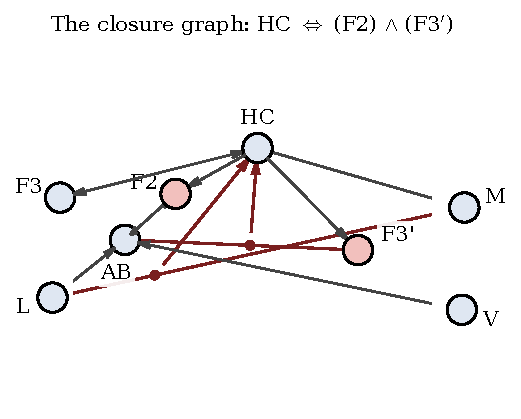
\includegraphics[width=0.92\textwidth]{figures/fig_graph}
\caption{The closure graph of Table~\ref{tab:rules}. Grey arrows are rules with one premise; a red fork joins the two premises of a rule that needs both. The coloured nodes are \Fii{} and \Fiii{}.}
\label{fig:graph}
\end{figure*}

\section{The algebraic locus in a family}\label{sec:loci}

\begin{definition}\label{def:algloc}
Let $\pi\colon\mathcal{X}\to S$ be a smooth projective morphism to a smooth connected complex quasi-projective variety, and let $\xi$ be a global section of $R^{2p}\pi_{*}\QQ$ that is a Hodge class at one point. The algebraic locus of $\xi$ is the set $\Sigma(\xi)$ of $s\in S$ at which $\xi_{s}\in H^{2p}(\mathcal{X}_{s})$ is algebraic.
\end{definition}

By the theorem of the fixed part \cite{Del71,And92}, the flat sections of a polarisable variation form a sub-Hodge structure, constant along $S$; so $\xi_{s}$ is a Hodge class at every point once it is one somewhere.

\begin{lemma}[Dichotomy]\label{lem:dichotomy}
\leavevmode
\begin{enumerate}[label=\textup{(\roman*)},leftmargin=2.4em,itemsep=2pt]
\item $\Sigma(\xi)$ is a countable union of Zariski closed subsets of $S$.
\item Either $\Sigma(\xi)=S$ or $\Sigma(\xi)$ is meagre in $S^{\mathrm{an}}$.
\item The following are equivalent: $\Sigma(\xi)=S$; $\Sigma(\xi)$ has an interior point; $\Sigma(\xi)$ is not meagre; $\xi_{s}$ is algebraic for the very general $s$. If $\Sigma(\xi)$ is dense they are equivalent to $\Sigma(\xi)$ being closed.
\end{enumerate}
\end{lemma}

\begin{proof}
(i) Fix a relatively ample line bundle on $\mathcal{X}$. For a Hilbert polynomial $P$ the relative Hilbert scheme $\mathrm{Hilb}^{P}(\mathcal{X}/S)$ is projective over $S$ \cite{Gro61}, and the class of the fibre of the universal family in $H^{2p}(\mathcal{X}_{s})$ is locally constant on each connected component of it, since a flat family of subschemes over a connected base has locally constant cycle class. A rational combination $\sum_{i}a_{i}[Z_{i}]$ equal to $\xi_{s}$ is a point of a fibre product $\prod_{S}\mathrm{Hilb}^{P_{i}}(\mathcal{X}/S)$, projective over $S$ and with countably many connected components; on each component the condition $\sum a_{i}[Z_{i}]=\xi$ is either empty or holds throughout, because both sides are flat sections. So $\Sigma(\xi)$ is the union, over the countably many tuples $(P_{i},a_{i})$ and components, of images of proper morphisms to $S$, each Zariski closed.

(ii) A countable union of proper Zariski closed subsets of an irreducible $S$ has empty interior in $S^{\mathrm{an}}$, and each is closed, so the union is meagre; if one of the closed sets is $S$ itself, $\Sigma(\xi)=S$.

(iii) By the Baire category theorem $S^{\mathrm{an}}$ is not meagre in itself, so $\Sigma(\xi)=S$ excludes meagreness, and a set with an interior point is not meagre; by (ii) not meagre forces $\Sigma(\xi)=S$. The complement of a countable union of proper closed subvarieties is the very general locus, so algebraicity at the very general point means that one of the closed sets is all of $S$. A dense set that is also closed is $S$.
\end{proof}

\begin{lemma}[Points of CM type are dense]\label{lem:cmdense}
Let $G$ be a connected reductive group over $\QQ$, $u_{0}\colon U(1)\to G_{\RR}$ a homomorphism and $\cD$ the orbit of $u_{0}$ under conjugation by $G(\RR)^{+}$. The points $u\in\cD$ for which $u(U(1))$ lies in the real points of a maximal torus of $G$ defined over $\QQ$ are dense in $\cD$.
\end{lemma}

\begin{proof}
Let $u_{1}\in\cD$ and $W$ a neighbourhood of $u_{1}$. A maximal torus $T_{1}$ of $G_{\RR}$ contains $u_{1}(U(1))$, since the centraliser of that compact torus is reductive and connected. Pick a regular element $Y_{1}$ in the Lie algebra $\mathfrak{t}_{1}$ of $T_{1}$. The map $(g,Y)\mapsto\mathrm{Ad}(g)Y$ from $G(\RR)^{+}\times\mathfrak{t}_{1}$ to $\mathfrak{g}_{\RR}$ is submersive at $(1,Y_{1})$ because $\mathfrak{g}_{\RR}=\mathfrak{t}_{1}\oplus[\mathfrak{g}_{\RR},Y_{1}]$, so the image of a small neighbourhood $N_{1}\times N_{2}$, with $N_{1}u_{1}N_{1}^{-1}\subseteq W$ and $N_{2}$ made of regular elements, contains an open set of $\mathfrak{g}_{\RR}$, hence a rational point $Y=\mathrm{Ad}(g)Y'$. The identity component $T$ of the centraliser of the rational regular semisimple $Y$ is a maximal torus over $\QQ$ with $T_{\RR}=gT_{1}g^{-1}$, and $u=gu_{1}g^{-1}\in W$ has $u(U(1))\subseteq T_{\RR}$.
\end{proof}

When $G=\Hg(A)$ and $u$ is the Hodge cocharacter of an abelian variety $A$, the condition of the lemma says that $\Hg(A)$ lies in a $\QQ$-torus, and then $A$ is of CM type: a maximal $\QQ$-torus of $\mathrm{GL}(H^{1}(A))$ containing it is the unit group of a commutative semisimple algebra $L$ of dimension $2\dim A$ commuting with $\Hg(A)$, and the commutant of $\Hg(A)$ is $\End^{0}(A)$.

\begin{proposition}[A family with a CM member through every Hodge class]\label{prop:cmfamily}
Let $A_{0}$ be an abelian variety and $\gamma$ a Hodge class on it. There are a polarised abelian scheme $\pi\colon\cA\to S$ over a smooth connected quasi-projective base, a flat section $\xi$ of $R^{2p}\pi_{*}\QQ$, a point $s_{0}$ with $\cA_{s_{0}}\cong A_{0}$ and $\xi_{s_{0}}=\gamma$, and a point $c$ with $\cA_{c}$ of CM type; the points of CM type are dense in $S$.
\end{proposition}

\begin{proof}
Let $G=\Hg(A_{0})$, let $u_{0}$ be the Hodge cocharacter of $A_{0}$ and $\cD$ its $G(\RR)^{+}$-orbit. Every $u\in\cD$ defines a polarisable Hodge structure of weight one on $H^{1}(A_{0})$ with Hodge group contained in $G$, so an abelian variety $A_{u}$ up to isogeny; fixing the lattice $H^{1}(A_{0},\ZZ)$, the polarisation of $A_{0}$ and a level structure of level $N\ge3$, the quotient $S=\Gamma\backslash\cD$ by a neat congruence subgroup $\Gamma\subseteq G(\QQ)$ is a smooth quasi-projective variety carrying a polarised abelian scheme with these fibres \cite{Mum69,Del71}. The class $\gamma$ is invariant under $G$, so it is a flat section $\xi$ of $R^{2p}\pi_{*}\QQ$, and $\xi_{s_{0}}=\gamma$ at the image $s_{0}$ of $u_{0}$. By Lemma~\ref{lem:cmdense} the points of CM type are dense in $\cD$, hence in $S$.
\end{proof}

\begin{theorem}[\Fii{} is propagation from CM points]\label{thm:propagation}
The following are equivalent.
\begin{enumerate}[label=\textup{(\roman*)},leftmargin=2.4em,itemsep=2pt]
\item \Fii{}.
\item $\AB$.
\item For every polarised abelian scheme $\pi\colon\cA\to S$ and every flat Hodge class $\xi$, algebraicity of $\xi_{s}$ at one point $s$ forces $\Sigma(\xi)=S$.
\item The same for the points $s$ of CM type.
\item For every $\pi$, $\xi$ with $\xi_{c}$ algebraic at a point $c$ of CM type, $\Sigma(\xi)$ has an interior point.
\end{enumerate}
\end{theorem}

\begin{proof}
(i) and (ii) are Theorem~\ref{thm:f2isab}. If (ii) holds, $\xi_{t}$ is a Hodge class at every $t$ by the theorem of the fixed part and algebraic by (ii), so (iii) holds; (iv) is a case of (iii), and (iv) and (v) are equivalent by Lemma~\ref{lem:dichotomy}(iii).

Assume (iv). Let $F$ be a CM field and $n\ge2$. The family of abelian varieties of split Weil type for $F$ over its Shimura variety is a polarised abelian scheme on which the Weil classes are flat sections, and by \cite[Thm.~1.1(i)]{BMB26} they are algebraic at a member isogenous to a product of abelian varieties with complex multiplication by $F$, a member of CM type; so by (iv) they are algebraic on every member, and by pull-back along an $F$-linear isogeny on every abelian variety of split Weil type for $F$. By Andr\'e's theorem, in the form Milne gives it \cite[Thm.~1 and \S5]{Mil20}, every Hodge class on an abelian variety of CM type is a sum of pull-backs, along homomorphisms, of Weil classes of abelian varieties of split Weil type; so $\AB$ holds for every abelian variety of CM type. Now let $A_{0}$ be any abelian variety and $\gamma$ a Hodge class on it, and take $\pi$, $\xi$, $s_{0}$, $c$ from Proposition~\ref{prop:cmfamily}. Then $\xi_{c}$ is algebraic, (iv) gives $\Sigma(\xi)=S$, and $\gamma=\xi_{s_{0}}$ is algebraic. This is (ii).
\end{proof}

\begin{proposition}[The Weil classes]\label{prop:weil-dense}
For every CM field $F$, every $n\ge2$ and every discriminant, the algebraic locus of the Weil classes in the polarised period domain $\cD_{F}$ contains an explicit point of CM type and is dense, and it is either $\cD_{F}$ or meagre.
\end{proposition}

\begin{proof}
This is \cite[Thm.~1.1]{BMB26}, items (i) to (iii). The density is the Hecke orbit of the base point: the group $G_{F}(\QQ)$ of the unitary group of the hermitian form acts on $\cD_{F}$ through $F$-linear isogenies that preserve the polarisation up to a scalar, hence preserve the algebraicity of the Weil classes, and its closure contains $G_{F}(\RR)^{+}$, which acts transitively. The dichotomy is Lemma~\ref{lem:dichotomy}.
\end{proof}

\begin{proposition}[\Fiii{} and the abelian part]\label{prop:abpart}
Let $H^{2p}_{\mathrm{ab}}(X)\subseteq H^{2p}(X)$ be the sum of the images of all maps $\Gamma_{*}\colon H^{k}(B)\to H^{2p}(X)$ with $B$ abelian and $\Gamma$ an algebraic cycle on $B\times X$. Then $H^{2p}_{\mathrm{ab}}(X)$ is a sub-Hodge structure, $\Ab^{p}(X)=\Hdg^{p}(X)\cap H^{2p}_{\mathrm{ab}}(X)$, and \Fiii{} holds for $X$ in degree $2p$ if and only if a Hodge complement $T^{2p}_{\mathrm{ab}}(X)$ of $H^{2p}_{\mathrm{ab}}(X)$ carries no nonzero Hodge class.
\end{proposition}

\begin{proof}
Each $\Gamma_{*}$ is a morphism of Hodge structures, so its image and the sum of finitely many images, which is all of $H^{2p}_{\mathrm{ab}}(X)$ by dimension, are sub-Hodge structures. A Hodge class in $H^{2p}_{\mathrm{ab}}(X)$ is $\sum\Gamma_{j*}y_{j}$, and the argument of Proposition~\ref{prop:f3prime-known}(i) replaces each $y_{j}$ by a Hodge class; so $\Ab^{p}(X)=\Hdg^{p}(X)\cap H^{2p}_{\mathrm{ab}}(X)$. A Hodge complement exists because the Hodge group is reductive, and the Hodge classes of $H^{2p}(X)$ are the direct sum of those of the two summands, which gives the last assertion.
\end{proof}

Theorem~\ref{thm:intro-loci} is Lemma~\ref{lem:dichotomy}, Theorem~\ref{thm:propagation}, Proposition~\ref{prop:weil-dense} and Proposition~\ref{prop:abpart}. Figure~\ref{fig:locus} draws the locus of Proposition~\ref{prop:weil-dense}.

\begin{figure}[t]
\centering
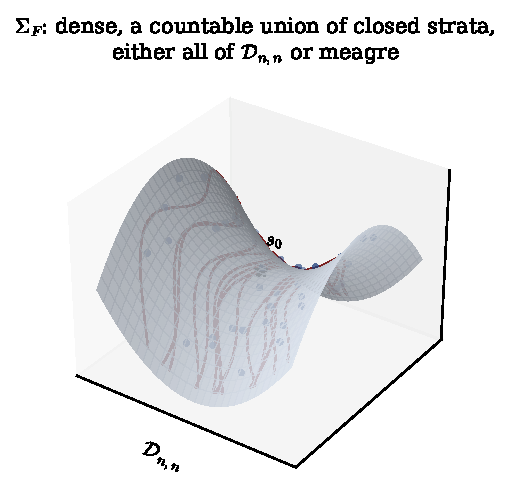
\includegraphics[width=0.95\columnwidth]{figures/fig_locus}
\caption{The period domain $\cD_{n,n}$ of a Weil family as a surface. The star is the CM base point, the dots and curves are strata of the algebraic locus, dense by the Hecke orbit. The locus is a countable union of closed strata; it is either the whole surface or meagre.}
\label{fig:locus}
\end{figure}

Both statements are now of one shape. There is a dense set of points at which the class is algebraic by an explicit cycle; the locus is a countable union of closed strata; the statement is that this union is not meagre, that is, that algebraicity propagates from the dense set. The rest of the paper goes to the first point where the propagation is not known and builds the object that would carry it.

\section{Constructions at \Fiii{}: real multiplication on K3 surfaces}\label{sec:f3prime}

\subsection{Where the first class is}

Let $S$ be a projective K3 surface, $T=T(S)_{\QQ}$ and $E=\End_{\Hdg}T$. The Hodge classes of $S\times S$ are $H^{0}\otimes H^{4}$, $H^{4}\otimes H^{0}$ and $\End_{\Hdg}H^{2}(S)=\End(\NS_{\QQ})\oplus E$, since $T$ is irreducible with no class of type $(1,1)$ and $\Hom_{\Hdg}(T,\NS_{\QQ})=0$. The first two pieces and $\End(\NS_{\QQ})$ are spanned by products of divisor classes. So the Hodge conjecture for $S\times S$ is the algebraicity of $E$, and by Proposition~\ref{prop:abpart} the same classes decide \Fiii{} for $S\times S$ once $T$ is not reached from abelian varieties. When $E$ is a CM field it is spanned by its elements of norm one, which are Hodge isometries of $T$ and algebraic by Buskin's theorem \cite{Bus19}; see \cite[Rem.~2.16]{Var23}. When $E$ is totally real, the Rosati involution is the identity on it \cite{Zar83}, every $e\in E$ is self-adjoint for the intersection form $q$, and $q(ex,ey)=q(e^{2}x,y)$. The first class is a real multiplication.

\subsection{Chains of correspondences}

\begin{lemma}\label{lem:dominant}
Let $f\colon S\dashrightarrow S'$ be a dominant rational map of K3 surfaces of degree $d$ and $\Gamma_{f}$ the closure of its graph. Then $f_{*}=\Gamma_{f*}$ and $f^{*}=\Gamma_{f*}^{t}$ are morphisms of Hodge structures, $f^{*}$ maps $T(S')_{\QQ}$ isomorphically onto $T(S)_{\QQ}$ with $q_{S}(f^{*}a,f^{*}b)=d\,q_{S'}(a,b)$, and $f_{*}=d\,(f^{*})^{-1}$ on $T(S)_{\QQ}$.
\end{lemma}

\begin{proof}
The graph is an algebraic cycle, so both maps are induced by algebraic classes and are morphisms of Hodge structures. Pull-back of a nowhere vanishing $2$-form is a nonzero $2$-form, so $f^{*}(T(S')_{\QQ})$ is a sub-Hodge structure of $H^{2}(S)$ that meets $H^{2,0}(S)$; the smallest sub-Hodge structure of $H^{2}(S)$ containing $H^{2,0}$ is $T(S)_{\QQ}$, so $f^{*}T(S')_{\QQ}\supseteq T(S)_{\QQ}$, and since $T(S')_{\QQ}$ is irreducible and $f^{*}$ is injective on it ($f_{*}f^{*}=d$), equality of dimensions gives $f^{*}T(S')_{\QQ}=T(S)_{\QQ}$. The projection formula gives $q_{S}(f^{*}a,f^{*}b)=q_{S'}(f_{*}f^{*}a,b)=d\,q_{S'}(a,b)$ and $f_{*}f^{*}=d$.
\end{proof}

\begin{lemma}\label{lem:isometry}
A Hodge isometry $\varphi\colon T(S)_{\QQ}\to T(S')_{\QQ}$ is induced by an algebraic class on $S\times S'$.
\end{lemma}

\begin{proof}
The spaces $\NS(S)_{\QQ}$ and $\NS(S')_{\QQ}$ are the orthogonal complements of $T(S)_{\QQ}$ and $T(S')_{\QQ}$ in the two copies of $\Lambda_{\QQ}$, isometric to each other through $\varphi$; by Witt's cancellation theorem the complements are isometric, so $\varphi$ extends to a Hodge isometry $H^{2}(S)\to H^{2}(S')$, which is algebraic by Buskin's theorem \cite{Bus19} (see \cite[Thm.~0.1]{Huy19}). The projector of $H^{2}(S)$ onto $T(S)_{\QQ}$ along $\NS(S)_{\QQ}$ is algebraic, being $1$ minus the projector onto $\NS$, which is a sum $\sum_{i,j}c_{ij}\,D_{i}\otimes D_{j}$ over a basis of divisor classes with $(c_{ij})$ the inverse Gram matrix; composing gives $\varphi$ on $T$ and zero on $\NS$.
\end{proof}

\begin{theorem}[Chains]\label{thm:chain}
Let $S$ be a projective K3 surface with $E$ totally real and $e\in E$ with $e^{2}=n\in\QQ_{>0}$. Suppose there are projective K3 surfaces $S=S_{0},S_{1},\dots,S_{r}$ and, for each $i$, either a dominant rational map $S_{i-1}\dashrightarrow S_{i}$ of degree $n_{i}$, a dominant rational map $S_{i}\dashrightarrow S_{i-1}$ of degree $n_{i}$, or a Hodge isometry $T(S_{i-1})_{\QQ}\cong T(S_{i})_{\QQ}$ (and then $n_{i}=1$), such that
\[
\prod_{i}n_{i}^{\pm1}\equiv n\pmod{\QQ^{\times2}},
\]
the sign being $+$ for maps leaving $S_{i-1}$ and $-$ for maps arriving at it. Then $e$ is algebraic on $S\times S$.
\end{theorem}

\begin{proof}
Composing along the chain the maps $f_{*}$ for maps leaving $S_{i-1}$, $f^{*}$ for maps arriving, and the classes of Lemma~\ref{lem:isometry} for the isometries, gives an algebraic isomorphism $\phi\colon T(S_{r})_{\QQ}\to T(S)_{\QQ}$ of Hodge structures with $q_{S}(\phi a,\phi b)=\mu\,q_{S_{r}}(a,b)$, where $\mu=\prod n_{i}^{\pm1}$ by Lemma~\ref{lem:dominant} (a map leaving contributes $f_{*}=n_{i}(f^{*})^{-1}$, of multiplier $n_{i}$; a map arriving contributes $f^{*}$, of multiplier $n_{i}$ in the other direction, that is $n_{i}^{-1}$ for the composite in the direction of $\phi$). Write $\mu=nc^{2}$ with $c\in\QQ^{\times}$. Since $e$ is self-adjoint with $e^{2}=n$, it is a Hodge similarity of $T(S)_{\QQ}$ of multiplier $n$. So $\psi=(c^{-1}\phi)^{-1}\circ e\colon T(S)_{\QQ}\to T(S_{r})_{\QQ}$ is a Hodge isometry, algebraic by Lemma~\ref{lem:isometry}, and $e=(c^{-1}\phi)\circ\psi$ is a composite of algebraic correspondences, hence algebraic on $S\times S$.
\end{proof}

The case $r=1$ with $S\dashrightarrow S_{1}$ the quotient by a symplectic automorphism of prime order $p$ is Varesco's theorem \cite[Thm.~2.1]{Var23}, which gives $e=\sqrt p$ and is used for $p=2,3$. What a chain adds is a composite multiplier.

\subsection{Real multiplication by $\QQ(\sqrt6)$}

A symplectic automorphism of finite order on a K3 surface acts trivially on $T(S)$, its quotient has a K3 resolution $Y$ \cite{Nik80}, and $T(Y)_{\QQ}\cong T(S)_{\QQ}(1/\mathrm{ord})$ by Lemma~\ref{lem:dominant}. The invariant lattice of a symplectic involution is $U^{3}\oplus E_{8}(-2)$, and a K3 surface has a symplectic involution exactly when $E_{8}(-2)$ embeds primitively in its N\'eron--Severi lattice \cite{Mor84,vGS07}. The invariant lattice of a symplectic automorphism of order three is $U\oplus U(3)^{2}\oplus A_{2}^{2}$, and such an automorphism exists exactly when the Coxeter--Todd lattice $K_{12}(-2)$ embeds primitively in the N\'eron--Severi lattice \cite[Thm.~4.1]{GS07}. Put
\[
V_{2}=\bigl(U^{3}\oplus E_{8}(-2)\bigr)_{\QQ},\qquad V_{3}=\bigl(U\oplus U(3)^{2}\oplus A_{2}^{2}\bigr)_{\QQ},
\]
of ranks $14$ and $10$ and signatures $(3,11)$ and $(3,7)$; over $\QQ$, $U(3)\cong U$ and $E_{8}(-2)\cong\langle-1\rangle^{8}\cong\langle-2\rangle^{8}$. Varesco \cite[Props.~2.5 and 2.11]{Var23} shows that a projective K3 surface whose transcendental space embeds isometrically in $V_{2}$ (resp.\ $V_{3}$) is Hodge isometric to one with a symplectic involution (resp.\ a symplectic automorphism of order three).

\begin{lemma}[Embedding criterion]\label{lem:embed}
Let $W$ and $V$ be rational quadratic spaces with $\mathrm{rk}\,V-\mathrm{rk}\,W\ge3$. Then $W$ embeds isometrically in $V$ if and only if the signature of $V$ dominates that of $W$ in both signs. In that case a complement $W'$ exists with $V\cong W\oplus W'$.
\end{lemma}

\begin{proof}
Necessity is clear. For sufficiency put $k=\mathrm{rk}\,V-\mathrm{rk}\,W\ge3$ and let $(s_{+},s_{-})$ be the difference of signatures, $s_{+}+s_{-}=k$. A quadratic space $W'$ of rank $k$ and signature $(s_{+},s_{-})$ with prescribed discriminant $d'=d(V)d(W)$ and prescribed Hasse invariants $\varepsilon_{p}'$ exists provided the $\varepsilon'_{p}$ equal $1$ for almost all $p$, $\prod_{p\le\infty}\varepsilon'_{p}=1$, and $\varepsilon'_{\infty}$, $d'$ match the signature \cite[Chap.~IV, Prop.~7]{Ser73}, with no further condition when $k\ge3$. Take $\varepsilon'_{p}=\varepsilon_{p}(V)\varepsilon_{p}(W)(d(W),d')_{p}$, the value forced by the formula $\varepsilon_{p}(W\oplus W')=\varepsilon_{p}(W)\varepsilon_{p}(W')(d(W),d(W'))_{p}$. The product formula for these holds because it holds for $V$, for $W$ and for the Hilbert symbol. Then $W\oplus W'$ and $V$ have the same rank, signature, discriminant and Hasse invariants at every place, so they are isometric by the Hasse--Minkowski theorem \cite[Chap.~IV, Thm.~9]{Ser73}, and $W$ embeds in $V$.
\end{proof}

\begin{theorem}[Two-dimensional families with algebraic real multiplication by $\QQ(\sqrt6)$]\label{thm:sqrt6}
Let $S$ be a projective K3 surface with $\QQ(\sqrt6)\subseteq E$ whose transcendental space $T=T(S)_{\QQ}$ embeds isometrically in $V_{3}$.
\begin{enumerate}[label=\textup{(\roman*)},leftmargin=2.4em,itemsep=2pt]
\item $\sqrt6\in E$ is algebraic on $S\times S$.
\item The Hodge conjecture, and \Fiii{}, hold for $S\times S$ and for the Hilbert square $S^{[2]}$.
\item Such surfaces exist in two-dimensional families, whose very general member has $\mathrm{rk}\,T=8$ and $E=\QQ(\sqrt6)$ exactly. One such family is the one whose transcendental space is $E^{4}$ with the trace form of $q_{E}=\langle-2,-2,-2+\sqrt6,-1+\sqrt6\rangle$ over $E=\QQ(\sqrt6)$.
\end{enumerate}
\end{theorem}

\begin{proof}
(i) By \cite[Prop.~2.11]{Var23} $S$ is Hodge isometric to a K3 surface $S'$ with a symplectic automorphism $\sigma$ of order three, and by Lemma~\ref{lem:isometry} the isometry is algebraic, so we may replace $S$ by $S'$. Let $Y$ be the minimal resolution of $S'/\sigma$ and $f_{1}\colon S'\dashrightarrow Y$ the quotient map, of degree three, so that $T(Y)_{\QQ}\cong T(1/3)$, of rank $\mathrm{rk}\,T\le8$ and signature $(2,\mathrm{rk}\,T-2)$: the rank is at most $8$ because $T$ embeds in $V_{3}$ of rank $10$ and signature $(3,7)$ with a complement that must contain the remaining positive direction, so the complement has rank at least two. Now $T(Y)_{\QQ}$ has rank at most $8$ and signature dominated by $(3,11)$, and $14-8\ge3$, so by Lemma~\ref{lem:embed} it embeds in $V_{2}$. By \cite[Prop.~2.5]{Var23} $Y$ is Hodge isometric to a K3 surface $Y'$ with a symplectic involution $\iota$; let $Z$ be the resolution of $Y'/\iota$ and $f_{2}\colon Y'\dashrightarrow Z$ the quotient, of degree two. The chain $S'\dashrightarrow Y\cong Y'\dashrightarrow Z$ has multiplier $3\cdot1\cdot2=6$, and Theorem~\ref{thm:chain} applies to $e=\sqrt6$ (Fig.~\ref{fig:chain}).

(ii) By the first paragraph of this section it remains to make $E$ algebraic. $E$ contains $\QQ(\sqrt6)$, and either $E=\QQ(\sqrt6)$ or $E$ is a CM field: a totally real $E$ has $\dim_{E}T\ge3$, because the complex line $H^{2,0}$ lies in one eigenspace $T_{\sigma}\otimes\CC$ and $\overline{H^{2,0}}$ in the same one, so that $T_{\sigma}\otimes\RR$ has signature $(2,\ast)$ and $\dim_{E}T\ge3$ follows from $q$ being negative definite on the other eigenspaces together with $T\otimes\RR$ having exactly two positive directions; and $[E:\QQ]\cdot\dim_{E}T=\mathrm{rk}\,T\le8$ then forces $[E:\QQ]\le2$. If $E=\QQ(\sqrt6)$, (i) suffices. If $E$ is CM, it is spanned by its norm-one elements, Hodge isometries, algebraic by Buskin's theorem. So every Hodge class on $S\times S$ is algebraic, and \Fiii{} follows. For $S^{[2]}$ the Chow motive is a direct summand of twists of $h(S\times S)$, $h(S)$ and $\mathbf{1}$ \cite{dCM02}, so every Hodge class on $S^{[2]}$ is the image under an algebraic correspondence of a Hodge class on $S\times S$ or $S$, and both statements follow.

(iii) Let $E=\QQ(\sqrt6)$ with real embeddings $\sigma_{1}$, $\sigma_{2}$ ($\sqrt6\mapsto\pm\sqrt6$), and let $q_{E}=\langle a_{1},a_{2},a_{3},a_{4}\rangle$ with $a_{1},a_{2}$ negative at both places and $a_{3},a_{4}$ positive at $\sigma_{1}$, negative at $\sigma_{2}$. The $\QQ$-space $T=E^{4}$ with the form $\Tr_{E/\QQ}\circ q_{E}$ has rank $8$ and signature $(2,2)+(0,4)=(2,6)$, and multiplication by $\sqrt6$ is self-adjoint of square $6$. For $q_{E}=\langle-2,-2,-2+\sqrt6,-1+\sqrt6\rangle$ one computes $d(T)=10$, $\varepsilon_{2}=1$, $\varepsilon_{3}=-1$, $\varepsilon_{5}=1$ and $\varepsilon_{p}=1$ otherwise, while $V_{3}$ has $d=-1$, $\varepsilon_{2}=1$, $\varepsilon_{3}=-1$, $\varepsilon_{5}=1$; and $T\oplus\langle1,-10\rangle$ has the invariants of $V_{3}$ at every place, so $V_{3}\cong T\oplus\langle1,-10\rangle$ by Hasse--Minkowski, with a complement containing a positive vector (Table~\ref{tab:invariants}; the Hilbert symbols are recomputed in the programs of Appendix~\ref{app:checks}). Embed $V_{3}$ in $\Lambda_{\QQ}$ as the invariant lattice of an order-three symplectic action, with orthogonal complement $K_{12}(-2)$, and let $N\subseteq\Lambda$ be the primitive sublattice with $N_{\QQ}=T^{\perp}$; it contains $K_{12}(-2)$ primitively and a positive class. The Hodge structures of K3 type on $T$ for which $\sqrt6$ is a Hodge endomorphism are the periods $\omega\in\PP(T_{\sigma_{1}}\otimes\CC)$ with $q(\omega)=0$, $q(\omega,\bar\omega)>0$, where $T_{\sigma_{1}}$ is the $\sigma_{1}$-eigenspace, of signature $(2,2)$; this is a domain of dimension two \cite[Prop.~2.3]{Var23}. For each such $\omega$ the surjectivity of the period map gives a K3 surface $S_{\omega}$ with $T(S_{\omega})_{\QQ}\subseteq T$, projective because $N$ contains a positive class, carrying an order-three symplectic automorphism because $K_{12}(-2)\subseteq N$ primitively. For $\omega$ outside a countable union of proper closed analytic subsets, $T(S_{\omega})_{\QQ}=T$ and $E=\QQ(\sqrt6)$, by the argument of \cite[Thm.~22.9]{BMB26}, which needs only $\dim_{E}T\ge3$.
\end{proof}

\begin{table}[t]
\centering
\caption{Rational invariants used in Theorem~\ref{thm:sqrt6}(iii). Hasse invariants are $+1$ at every prime not shown.}
\label{tab:invariants}
\begin{ruledtabular}
\begin{tabular}{lcccccc}
space & rank & signature & $d$ & $\varepsilon_{2}$ & $\varepsilon_{3}$ & $\varepsilon_{5}$ \\
\colrule
$T=\Tr_{E/\QQ}q_{E}$ & 8 & $(2,6)$ & $10$ & $+1$ & $-1$ & $+1$ \\
$\langle1,-10\rangle$ & 2 & $(1,1)$ & $-10$ & $+1$ & $+1$ & $+1$ \\
$T\oplus\langle1,-10\rangle$ & 10 & $(3,7)$ & $-1$ & $+1$ & $-1$ & $+1$ \\
$V_{3}$ & 10 & $(3,7)$ & $-1$ & $+1$ & $-1$ & $+1$ \\
$V_{2}$ & 14 & $(3,11)$ & $-1$ & $-1$ & $+1$ & $+1$ \\
\end{tabular}
\end{ruledtabular}
\end{table}

\begin{figure}[t]
\centering
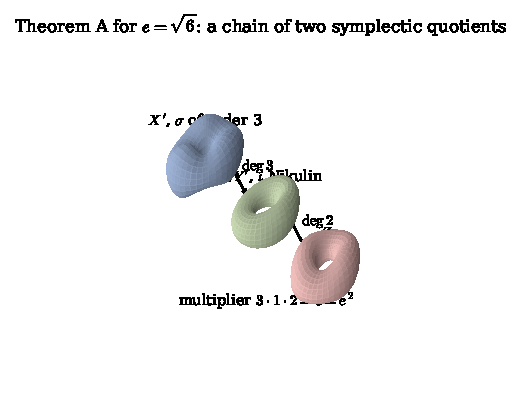
\includegraphics[width=0.95\columnwidth]{figures/fig_chain}
\caption{The chain of Theorem~\ref{thm:sqrt6}: the quotient of $S'$ by a symplectic automorphism of order three, a Hodge isometry (algebraic by Buskin), and the quotient of $Y'$ by a Nikulin involution. The multipliers compose to $6$.}
\label{fig:chain}
\end{figure}

Varesco's families have $E=\QQ(\sqrt2)$ or $\QQ(\sqrt3)$ \cite[Thms.~2.9, 2.15]{Var23}; van Geemen and Sch\"utt obtain $\sqrt2$, $\sqrt3$, $\sqrt7$ from rational self-maps of elliptic K3 surfaces \cite[\S\S6--7]{vGS25}; Bayer-Fluckiger, van Geemen and Sch\"utt prove that families with real multiplication by any totally real $E$ with $[E:\QQ]\dim_{E}T\le21$ exist, without algebraicity \cite{BvGS24}. The lattice condition of Theorem~\ref{thm:sqrt6} is a genuine restriction: among the $165$ sign-admissible diagonal forms $q_{E}$ with small coefficients, $98$ embed in $V_{3}$ and $67$ do not (Appendix~\ref{app:checks}).

\subsection{Isogenies of elliptic surfaces}\label{ssec:fricke}

Varesco's quotients and the chains of Theorem~\ref{thm:chain} produce the square roots of the orders of symplectic automorphisms, $2$ and $3$, and their products. A different source of similarities is a rational self-map of a K3 surface, and the self-maps that exist in families come from isogenies of elliptic fibrations: van Geemen and Sch\"utt obtain $\sqrt2$ and $\sqrt3$ from isogenies of degree $2$ and $3$ in this way, and for degrees $5$ and $7$ they give one surface each \cite[\S\S6--7]{vGS25}. We show that the degrees $5$ and $7$ also come in families.

Let $N\in\{5,7\}$ and write $N^{k}$ for $125$ when $N=5$ and $49$ when $N=7$. The modular curve $X_{0}(N)$ is rational, with Fricke's coordinate $t$ in which the involution $(E,C)\mapsto(E/C,E[N]/C)$ is $w(t)=N^{k}/t$ \cite[\S7.6]{vGS25}. The universal curve with a cyclic subgroup $C_{t}$ of order $N$ over $\PP^{1}_{t}$ is
\begin{equation}\label{eq:fricke}
\mathcal{E}_{t}\colon\ y^{2}=x^{3}-27c_{4}(t)\,x-54c_{6}(t),
\end{equation}
with, for $N=7$,
\begin{align*}
c_{4}&=(t^{2}+13t+49)(t^{2}+5t+1),\\
c_{6}&=(t^{2}+13t+49)(t^{4}+14t^{3}+63t^{2}+70t-7),
\end{align*}
and for $N=5$,
\begin{align*}
c_{4}&=(t^{2}+10t+5)(t^{2}+22t+125),\\
c_{6}&=(t^{2}+4t-1)(t^{2}+22t+125)^{2}.
\end{align*}
The discriminant is $1728\,t\,(t^{2}+13t+49)^{2}$ for $N=7$ and $1728\,t\,(t^{2}+22t+125)^{3}$ for $N=5$, of degree $5$ and $7$. So the relatively minimal model $R_{N}$ of \eqref{eq:fricke} over $\PP^{1}_{t}$ is a rational elliptic surface with fibres of type $\mathrm{I}_{1}$ at $t=0$, $\mathrm{I}_{N}$ at $t=\infty$, and at the two roots $e_{1},e_{2}$ of the quadratic factor, where $c_{4}$ vanishes, of type $\mathrm{II}$ for $N=7$ and $\mathrm{III}$ for $N=5$; the Euler numbers add up to $1+N+2\cdot2=12$ and $1+N+2\cdot3=12$. The roots satisfy $e_{1}e_{2}=N^{k}$, so $w$ exchanges them and exchanges $0$ with $\infty$.

\begin{lemma}[The Fricke isogeny over the function field]\label{lem:fricke}
$\mathcal{E}_{t}/C_{t}\cong\mathcal{E}_{w(t)}$ over $\CC(t)$.
\end{lemma}

\begin{proof}
The two curves have the same $j$-invariant, because $w$ is the Fricke involution of $X_{0}(N)$. Two elliptic curves over $\CC(t)$ with the same non-constant $j$-invariant differ by a quadratic twist $\chi\in\CC(t)^{\times}/\CC(t)^{\times2}$, and a twist ramified at a point of $\PP^{1}$ changes the Kodaira type of the fibre there, exchanging $\mathrm{I}_{n}$ with $\mathrm{I}_{n}^{*}$, $\mathrm{II}$ with $\mathrm{IV}^{*}$ and $\mathrm{III}$ with $\mathrm{III}^{*}$. So it suffices to show that $\mathcal{E}_{t}/C_{t}$ has the same fibre types as $\mathcal{E}_{w(t)}$, which are $\mathrm{I}_{N}$ at $0$, $\mathrm{I}_{1}$ at $\infty$ and $\mathrm{II}$ or $\mathrm{III}$ at $e_{1},e_{2}$: then $\chi$ is unramified on $\PP^{1}$, hence constant, hence trivial over $\CC$.

At $t=0$ the fibre of $\mathcal{E}$ is $\mathrm{I}_{1}$, the Tate curve $\mathbb{G}_{m}/q^{\ZZ}$ over $\CC((t))$, whose only cyclic subgroup of order $N$ rational over $\CC((t))$ is $\mu_{N}$; the quotient $\mathbb{G}_{m}/q^{N\ZZ}$ is $\mathrm{I}_{N}$. At $e_{i}$ the local monodromy $M\in\SL_{2}(\ZZ)$ of $\mathcal{E}$ has order $6$ or $4$ and irreducible characteristic polynomial; the isogeny is given on the period lattices by a matrix $A\in M_{2}(\ZZ)$ with $\det A=N$, and the monodromy of the quotient is $M'=AMA^{-1}$. The $\SL_{2}(\ZZ)$-classes with this characteristic polynomial are those of $M$ and $M^{-1}$, which are the types $\mathrm{II}$ and $\mathrm{II}^{*}$, or $\mathrm{III}$ and $\mathrm{III}^{*}$. If $M'=gM^{-1}g^{-1}$ with $g\in\SL_{2}(\ZZ)$, then $B=g^{-1}A$ conjugates $M$ to $M^{-1}$. All rational matrices doing so form the coset $B_{0}\,\QQ(M)^{\times}$, where $B_{0}=\bigl(\begin{smallmatrix}0&1\\1&0\end{smallmatrix}\bigr)$ for $M=\bigl(\begin{smallmatrix}0&-1\\1&\mathrm{tr}M\end{smallmatrix}\bigr)$ has determinant $-1$ and the elements of the imaginary quadratic field $\QQ(M)$ have positive norm; so $\det B<0$, against $\det B=N$. Hence the quotient has the type of $M$ at $e_{1},e_{2}$. At $\infty$ the $j$-invariant of the quotient has a simple pole, so the fibre is $\mathrm{I}_{1}$ or $\mathrm{I}_{1}^{*}$, and the Euler numbers of the other fibres add up to $11$; since the total is $12$ the fibre is $\mathrm{I}_{1}$.
\end{proof}

For $p\ne q$ in $\PP^{1}_{t}$ let $u_{p,q}=(t-p)(t-q)$, and let $X_{p,q}$ be the elliptic K3 surface whose generic fibre is the quadratic twist $\mathcal{E}_{t}\otimes u_{p,q}$: the twist multiplies $c_{4}$ by $u^{2}$ and $c_{6}$ by $u^{3}$, giving Weierstrass coefficients of degrees $8$ and $12$, and adds two fibres of type $\mathrm{I}_{0}^{*}$ at $p$ and $q$ when these are not among $0,\infty,e_{1},e_{2}$. For a double cover $\psi\colon\PP^{1}_{s}\to\PP^{1}_{t}$ let $X_{\psi}$ be the relatively minimal model of $\psi^{*}\mathcal{E}$.

\begin{lemma}\label{lem:twists}
\leavevmode
\begin{enumerate}[label=\textup{(\roman*)},leftmargin=2.4em,itemsep=2pt]
\item $X_{p,q}$ has Picard number at least $16$: its Néron--Severi lattice contains $U\oplus A_{6}\oplus D_{4}^{2}$ for $N=7$ and $U\oplus A_{4}\oplus A_{1}^{2}\oplus D_{4}^{2}$ for $N=5$. The same bound holds for $X_{\psi}$, whose fibres $2\,\mathrm{I}_{1}+2\,\mathrm{I}_{N}$, together with four fibres of type $\mathrm{III}$ when $N=5$, and the pulled-back Mordell--Weil group of $R_{N}$, of rank $2$, give rank at least $16$ by the Shioda--Tate formula.
\item The fibrewise isogeny by $C_{t}$ is a dominant rational map of degree $N$
\[
f\colon X_{p,q}\dashrightarrow X_{w(p),w(q)},\qquad f\colon X_{\psi}\dashrightarrow X_{w\circ\psi}.
\]
\item The deck involution of $\psi$ times $[-1]$ on the fibres is a symplectic involution $\iota$ of $X_{\psi}$, and the minimal resolution of $X_{\psi}/\iota$ is $X_{p,q}$ with $\{p,q\}$ the branch locus of $\psi$. Hence $T(X_{\psi})_{\QQ}\cong T(X_{p,q})_{\QQ}(1/2)$ as in Lemma~\ref{lem:dominant}, and the two surfaces have the same Picard number.
\end{enumerate}
\end{lemma}

\begin{proof}
(i) Shioda--Tate with the fibres listed, and for $X_{\psi}$ the Mordell--Weil rank $8-6=2$ of $R_{N}$. (ii) By Lemma~\ref{lem:fricke} the quotient of the generic fibre is $\mathcal{E}_{w(t)}\otimes u_{p,q}(t)$, and
\[
u_{p,q}(w(t))=\Bigl(\frac{N^{k}}{t}-p\Bigr)\Bigl(\frac{N^{k}}{t}-q\Bigr)=\frac{pq}{t^{2}}\,u_{w(p),w(q)}(t),
\]
a constant times a square times $u_{w(p),w(q)}$. So $\mathcal{E}_{w(t)}\otimes u_{p,q}(t)\cong\mathcal{E}_{w(t)}\otimes u_{w(p),w(q)}(w(t))$, which is the pull-back along the automorphism $w$ of the base of the generic fibre of $X_{w(p),w(q)}$; pulling back along an automorphism of the base gives an isomorphic surface. For $X_{\psi}$, $(\psi^{*}\mathcal{E})/C=\psi^{*}(\mathcal{E}/C)\cong\psi^{*}w^{*}\mathcal{E}$. (iii) The quadratic twist by the function defining the double cover is the quotient of the base change by the deck involution composed with $[-1]$ on the fibres; the involution is symplectic with eight fixed points, the $2$-torsion of the two fibres over the ramification points, and the quotient's resolution is the twist.
\end{proof}

\begin{theorem}[One-dimensional families with algebraic real multiplication by $\sqrt5$ and $\sqrt7$]\label{thm:fricke}
Let $N\in\{5,7\}$ and let $\mathfrak{A}_{N}$ be the family of surfaces $X_{p}=X_{p,N^{k}/p}$ for $p\notin\{0,\infty,e_{1},e_{2},\pm\sqrt{N^{k}}\}$, and $\mathfrak{B}_{N}$ the family of surfaces $X_{\psi}$ with $\psi$ branched over a pair $\{b,N^{k}/b\}$.
\begin{enumerate}[label=\textup{(\roman*)},leftmargin=2.4em,itemsep=2pt]
\item Every member $X$ has a dominant rational self-map $f$ of degree $N$, and $f^{*}$ is an element of $E=\End_{\Hdg}T(X)_{\QQ}$ with $f^{*}f_{*}=N$.
\item The families are not isotrivial. Their very general member has Picard number $16$, transcendental rank $6$ and $E=\QQ(\sqrt N)$, with $\sqrt N=\pm f^{*}$ algebraic on $X\times X$.
\item For every member $X$ the Hodge conjecture holds for $X\times X$, and \Fiii{} holds for $X\times X$ and for $X^{[2]}$.
\end{enumerate}
\end{theorem}

\begin{proof}
(i) $w$ exchanges $p$ and $N^{k}/p$, so Lemma~\ref{lem:twists}(ii) gives $f\colon X_{p}\dashrightarrow X_{p}$; for $\mathfrak{B}_{N}$, $w\circ\psi$ has the same branch locus as $\psi$, so $w\circ\psi=\psi\circ\sigma$ for a M\"obius transformation $\sigma$ and $X_{w\circ\psi}\cong X_{\psi}$. The correspondence of a dominant rational map preserves $\NS$ and its transpose does too, so it preserves $T=\NS^{\perp}$ and acts there as a morphism of Hodge structures, nonzero since $f^{*}\omega=\lambda\omega$ with $\lambda\ne0$; on a resolution $S$ of the graph with $p_{1}\colon S\to X$ birational and $p_{2}$ of degree $N$, both $p_{1}^{*}T$ and $p_{2}^{*}T$ are irreducible sub-Hodge structures of $H^{2}(S)$ containing its unique $(2,0)$-line, so they coincide, and $f_{*}f^{*}=p_{2*}p_{1}^{*}p_{1*}p_{2}^{*}=N$ on $T$.

(ii) The elliptic fibration of $X_{p}$ has labelled singular fibres $\mathrm{I}_{1}$ at $0$, $\mathrm{I}_{N}$ at $\infty$, $\mathrm{II}$ or $\mathrm{III}$ at $e_{1},e_{2}$ and $\mathrm{I}_{0}^{*}$ at $p$ and $N^{k}/p$. An isomorphism of elliptic fibrations induces a M\"obius transformation preserving this configuration; the transformations preserving $\{0,\infty\}$ and $\{e_{1},e_{2}\}$ are $t\mapsto\lambda t$ and $t\mapsto\lambda/t$ with $\lambda e_{1}\in\{e_{1},e_{2}\}$, and since $e_{1}+e_{2}\ne0$ and $e_{1}^{2}\ne e_{2}^{2}$ they are the identity and $w$, which preserve $\{p,N^{k}/p\}$. So $X_{p}$ and $X_{p'}$ have isomorphic fibrations only when $p'\in\{p,N^{k}/p\}$. A K3 surface has finitely many elliptic fibrations up to automorphisms \cite{Ste85}, so the map $p\mapsto[X_{p}]$ to the moduli space has finite fibres and the family is not isotrivial; by local Torelli its period map has uncountable image. A Hodge structure of K3 type on a fixed rational quadratic space with $E$ a CM field is determined by $E$, a subalgebra of the endomorphism algebra, and by an eigenline of $E\otimes\CC$, so there are countably many; the very general member is therefore not of CM type, and its $E$ is totally real. It contains $f^{*}$, and $f_{*}=N(f^{*})^{-1}$ is the adjoint of $f^{*}$, equal to $f^{*}$ since the adjoint involution is trivial on a totally real $E$; so $(f^{*})^{2}=N$ and $E\ne\QQ$. A totally real $E\ne\QQ$ has $\dim_{E}T\ge3$ \cite{vG08}, so $\mathrm{rk}\,T\ge6$; with $\rho\ge16$ this gives $\mathrm{rk}\,T=6$, $\rho=16$, $[E:\QQ]=2$ and $E=\QQ(\sqrt N)$. The same holds for $\mathfrak{B}_{N}$ by Lemma~\ref{lem:twists}(iii).

(iii) For every member $E\supseteq\QQ(\sqrt N)$ and $\mathrm{rk}\,T\le6$. If $E$ is totally real then $\dim_{E}T\ge3$ forces $E=\QQ(\sqrt N)=\QQ+\QQ f^{*}$, algebraic. Otherwise $E$ is a CM field, and every element of $E$ of norm one to its real subfield is a Hodge isometry of $T$, extended by the identity on $\NS$ to a Hodge isometry of $H^{2}(X,\QQ)$, algebraic by Buskin's theorem \cite{Bus19}. The algebraic classes form a $\QQ$-subalgebra $E'\subseteq E$ containing these elements; for $x\in E$ with $\bar x\ne x$ and $t_{1}\ne t_{2}$ in $\QQ$ it contains $(t_{i}+x)/(t_{i}+\bar x)$, hence their quotient $1+(t_{2}-t_{1})/(t_{1}+\bar x)$, hence $\bar x$; so $E'=E$. In both cases $\End_{\Hdg}H^{2}(X)=\End(\NS)\oplus E$ is algebraic, and $\Hdg^{2}(X\times X)=\End_{\Hdg}H^{2}(X)\oplus H^{0}\otimes H^{4}\oplus H^{4}\otimes H^{0}$ since $H^{1}=H^{3}=0$; the Hodge conjecture holds for $X\times X$, which gives \Fiii{} there, and passes to $X^{[2]}$ by \cite{dCM02}.
\end{proof}

\begin{figure}[t]
\centering
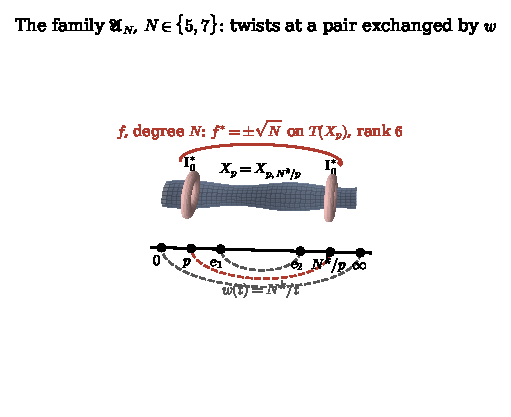
\includegraphics[width=0.95\columnwidth]{figures/fig_fricke}
\caption{The family $\mathfrak{A}_{N}$ of Theorem~\ref{thm:fricke}. Over the Fricke coordinate $t$ of $X_{0}(N)$ the involution $w(t)=N^{k}/t$ exchanges the cusps $0$, $\infty$ and the elliptic points $e_{1}$, $e_{2}$; the twist $X_{p}$ at a pair $\{p,N^{k}/p\}$ exchanged by $w$ is carried to itself by the fibrewise isogeny $f$ of degree $N$, and $f^{*}$ is the real multiplication by $\sqrt N$ on the transcendental lattice of rank six.}
\label{fig:fricke}
\end{figure}

The surface of \cite[\S7.6]{vGS25} with real multiplication by $\sqrt7$ is the twist at $\{7,-7\}$, the two fixed points of $w$, and the surface of \cite[Prop.~7.7]{vGS25} is the twist at the fixed points $\pm5\sqrt5$ for $N=5$, which has Picard number $18$ and complex multiplication. The families $\mathfrak{A}_{N}$ are the twists at the pairs exchanged by $w$; they are one-dimensional, their very general member has real and not complex multiplication, and for $N=5$ they are the first K3 surfaces of transcendental rank six with real multiplication by $\sqrt5$ that we know to carry an algebraic $\sqrt5$. The chains of Theorem~\ref{thm:chain} apply to every member: a transcendental space of rank six embeds in $V_{2}$ and $V_{3}$ with any rational scaling, so a member whose $E$ happened to contain $\sqrt{2N}$, $\sqrt{3N}$ or $\sqrt{6N}$ would have that element algebraic as well. We do not know such a member: the twist families of fixed Picard number $16$ are two-dimensional, the real multiplication loci for a fixed quadratic field on a transcendental space of rank six are one-dimensional inside a four-dimensional period domain, and the intersection has expected dimension $-1$.

\subsection{The reach of similarities}

Every correspondence used so far acts on transcendental spaces as a Hodge similarity. The next proposition says that this is not an accident of the examples but a property of every correspondence whose components are small, and it measures what a correspondence must look like to act otherwise.

\begin{proposition}[Structure of the transcendental action]\label{prop:structure}
Let $X$, $X'$ be projective K3 surfaces, $\Gamma\in\mathrm{CH}^{2}(X\times X')_{\QQ}$, and $\gamma_{T}\colon T(X)_{\QQ}\to T(X')_{\QQ}$ the map induced on transcendental spaces by composing the action of $\Gamma$ with the orthogonal projections.
\begin{enumerate}[label=\textup{(\roman*)},leftmargin=2.4em,itemsep=2pt]
\item $\gamma_{T}$ is zero or an isomorphism of Hodge structures.
\item If $\gamma_{T}\ne0$ then $a=\gamma_{T}^{\dagger}\gamma_{T}$ lies in the maximal totally real subfield of $E=\End_{\Hdg}T(X)_{\QQ}$ and is totally positive, and $\gamma_{T}$ is a similarity exactly when $a\in\QQ$.
\item Let $\Gamma$ be irreducible, $S$ a resolution of its normalisation with projections $p_{1},p_{2}$ of degrees $d_{1},d_{2}$ to $X$, $X'$. If $p_{1}^{*}T(X)_{\QQ}=p_{2}^{*}T(X')_{\QQ}$ inside $H^{2}(S,\QQ)$, then $\gamma_{T}$ is a similarity of multiplier $d_{1}d_{2}$. This holds whenever $p_{g}(S)\le1$.
\item If $\Gamma$ is irreducible and $\gamma_{T}$ is not a similarity, then $p_{1}^{*}T(X)_{\QQ}\cap p_{2}^{*}T(X')_{\QQ}=0$, so $p_{g}(S)\ge2$ and the transcendental rank of $S$ is at least twice that of $X$.
\item The $\QQ$-algebra generated by the actions on $T(X)_{\QQ}$ of all correspondences from $X$ to itself whose irreducible components either fail to dominate a factor or have $p_{g}\le1$ is the multiquadratic subfield $E_{2}\subseteq E$ generated by the square roots of the products $d_{1}d_{2}$ that occur. When $[E:\QQ]$ is odd it is $\QQ$.
\end{enumerate}
\end{proposition}

\begin{proof}
(i) $T(X)_{\QQ}$ is an irreducible Hodge structure \cite{Zar83}, and the image of $\gamma_{T}$ is a sub-Hodge structure of $H^{2}(X')$; if nonzero it contains the $(2,0)$-part, hence $T(X')_{\QQ}$, and $\gamma_{T}$ is injective by irreducibility. (ii) $a$ is a Hodge endomorphism of $T(X)$, so $a\in E$, and it is self-adjoint, so it lies in the fixed field of the adjoint involution, the maximal totally real subfield. The form $q'(\gamma x,\gamma y)=q(x,ay)$ is a polarisation of the Hodge structure $T(X)$ up to sign on each real eigenspace of $E$, and comparison with $q$ gives $\sigma(a)>0$ at every real place. A similarity of multiplier $\mu$ has $a=\mu$. (iii) Both $p_{i}^{*}T$ are irreducible sub-Hodge structures of $H^{2}(S)$ with a $(2,0)$-part; if $p_{g}(S)\le1$ they share the unique $(2,0)$-line, so they meet and coincide. When they coincide, $\gamma_{T}=p_{2*}p_{1}^{*}=d_{2}(p_{2}^{*})^{-1}p_{1}^{*}$ on $T$, so $p_{2}^{*}\gamma x=d_{2}\,p_{1}^{*}x$; since $q_{S}(p_{1}^{*}x,p_{1}^{*}y)=d_{1}q(x,y)$ and $q_{S}(p_{2}^{*}x',p_{2}^{*}y')=d_{2}q'(x',y')$, this gives $d_{2}\,q'(\gamma x,\gamma y)=q_{S}(p_{2}^{*}\gamma x,p_{2}^{*}\gamma y)=d_{2}^{2}\,q_{S}(p_{1}^{*}x,p_{1}^{*}y)=d_{1}d_{2}^{2}\,q(x,y)$, that is $q'(\gamma x,\gamma y)=d_{1}d_{2}\,q(x,y)$. (iv) If the two subspaces met they would coincide by irreducibility and (iii) would apply; so they are independent, their $(2,0)$-lines are distinct, and their sum has rank $2\,\mathrm{rk}\,T(X)$ inside the transcendental part of $H^{2}(S)$. (v) A component that does not dominate a factor acts through $\NS$ or through $H^{0}$ and $H^{4}$, hence by zero on $T$. The others act by similarities by (iii), a composite of similarities returning to $X$ is an element $\Phi\in E$ with $\Phi^{\dagger}\Phi\in\QQ$, and for totally real $E$ this is $\Phi^{2}\in\QQ$; such elements generate $E_{2}$. For a CM field $E$ the elements with $\Phi^{\dagger}\Phi\in\QQ$ are the $\QQ^{\times}$-multiples of the norm-one elements, which generate $E$, so the statement is about the totally real case, which is the one that matters for \Fiii{}. An odd-degree field has $E_{2}=\QQ$.
\end{proof}

The correspondences of Lemmas~\ref{lem:dominant} and \ref{lem:isometry}, the Fourier--Mukai kernels between a K3 surface and its moduli spaces of sheaves, the rational Hodge isometries of hyper-K\"ahler varieties of K3$^{[n]}$ type \cite{Mar24}, the Fricke isogenies of Theorem~\ref{thm:fricke} and all their composites fall under (iii) or (v). A correspondence that realises an element of a cubic field must therefore have a component whose resolution has $p_{g}\ge2$ and transcendental rank at least twice that of the surface. Such correspondences exist, and the only ones we know come from finite groups.

\begin{proposition}[Hecke correspondences]\label{prop:hecke}
Let $Z$ be a smooth projective surface with an action of a finite group $G$, $H\le G$ a subgroup, and $X$ a smooth projective surface with $p_{g}(X)=1$ birational to $Z/H$; write $\pi\colon Z\dashrightarrow X$.
\begin{enumerate}[label=\textup{(\roman*)},leftmargin=2.4em,itemsep=2pt]
\item For $g\in G$ the correspondence $\Gamma_{g}=(\pi\times\pi)_{*}[\text{graph of }g]$ acts on $H^{2}(X,\QQ)$ as the Hecke operator of the double coset $HgH$, and these operators span a $\QQ$-algebra isomorphic to a quotient of $\End_{G}\QQ[G/H]$ acting by Hodge endomorphisms.
\item Exactly one simple factor of this algebra acts nontrivially on $H^{2,0}(X)$; it is a field, it preserves $T(X)_{\QQ}$, and it embeds into $E$ by algebraic correspondences. If $H^{2,0}(Z)^{G}=0$ this factor is not the one on which $G$ acts trivially.
\item Every field obtained in this way is abelian over $\QQ$. In particular a totally real cubic field $F$ whose Galois closure has group $S_{3}$ is realised by no correspondence built from a finite group acting on a cover of $X$.
\end{enumerate}
\end{proposition}

\begin{proof}
(i) Let $\tilde Z\to Z$ be an equivariant resolution and $\pi\colon\tilde Z\to X$ the quotient by $H$ followed by the resolution; then $\pi_{*}\pi^{*}=|H|$ and $\pi_{*}h^{*}=\pi_{*}$ for $h\in H$, so $\Gamma_{g}$ acts as $\pi_{*}g^{*}\pi^{*}=(\pi^{*})^{-1}\circ\sum_{h\in HgH/H}h^{*}\circ\pi^{*}$ on $H^{2}(X,\QQ)=H^{2}(\tilde Z,\QQ)^{H}$, the Hecke operator of $HgH$. The Hecke operators of $(G,H)$ span $\End_{G}\QQ[G/H]$, a semisimple algebra, and the action on $H^{2}(\tilde Z,\QQ)^{H}$ factors through it. (ii) The idempotents of the simple factors are rational combinations of Hecke operators, so they are Hodge endomorphisms of $H^{2}(X)$; they sum to $1$ and act on the line $H^{2,0}(X)$ by $0$ or $1$, so exactly one of them, $e_{V}$, acts as $1$. A simple factor with nonzero image in the commutative ring $\End_{\Hdg}H^{2,0}(X)=\CC$ through a ring homomorphism to a field is commutative, hence a field $\mathcal{H}_{V}$. For $f\in\mathcal{H}_{V}$, $f(T(X)_{\QQ})$ is a sub-Hodge structure of the transcendental part of $H^{2}(X)$; if $f\omega\ne0$ it contains $\omega$, hence $T(X)_{\QQ}$, and if $f\omega=0$ it has no $(2,0)$-part and lies in $\NS\cap T=0$. So $\mathcal{H}_{V}\to\End_{\Hdg}T(X)_{\QQ}=E$ is a homomorphism from a field, injective. The factor on which $G$ acts trivially fixes $H^{2,0}(\tilde Z)^{G}=H^{2,0}(Z/G)$, which is zero by hypothesis, so it is not $\mathcal{H}_{V}$. (iii) The centres of the simple factors of $\End_{G}\QQ[G/H]$ are the character fields $\QQ(\chi_{i})$ of the irreducible constituents of $\QQ[G/H]$, generated by sums of roots of unity, so each lies in $\QQ(\zeta_{|G|})$ and is abelian; a commutative simple factor is its centre. A non-abelian cubic field is not a subfield of an abelian field.
\end{proof}

For the dihedral group $D_{n}$ with $n$ odd, $H=\langle\tau\rangle$ of order two and $Z$ the elliptic surfaces $\tilde{\mathcal{E}}_{a}$ of \cite[\S4.7]{vGS25}, the algebra $\End_{D_{n}}\QQ[D_{n}/H]$ is $\QQ\times\prod_{d\mid n,\,d>1}\QQ(\zeta_{d})^{+}$, and the factor acting on $\omega$ is $\QQ(\zeta_{n})^{+}$; this is the content of \cite[\S4.8]{vGS25}, where the cycle $\Gamma_{1}+\Gamma_{-1}$ induces $\zeta_{n}+\zeta_{n}^{-1}$. The components of these correspondences are birational to $\tilde{\mathcal{E}}_{a}$, which has $p_{g}\ge2$, as Proposition~\ref{prop:structure}(iv) requires.

\begin{corollary}[Squares of the dihedral families]\label{cor:dihedral}
Let $X$ be an elliptic K3 surface of one of the families of \cite[Thm.~1.1]{vGS25}, with real multiplication by $F=\QQ(\zeta_{n})^{+}$ for $n\in\{5,7,9,11\}$, and suppose $E=F$ or $E$ is a CM field; the very general member has $E=F$. Then the Hodge conjecture holds for $X\times X$, and \Fiii{} holds for $X\times X$ and $X^{[2]}$. This covers the cubic fields $\QQ(\zeta_{7})^{+}$ and $\QQ(\zeta_{9})^{+}$ on families of dimensions $3$ and $2$.
\end{corollary}

\begin{proof}
If $E=F$, $E$ is algebraic by Proposition~\ref{prop:hecke}(ii) and \cite[\S4.8]{vGS25}; if $E$ is CM, by Buskin's theorem as in Theorem~\ref{thm:fricke}(iii). The rest is as there.
\end{proof}

\subsection{Where this stops}\label{ssec:f3stop}

The frontier case of \Fiii{} in \cite[Thm.~21.4 and Rem.~21.5]{BMB26} is a K3 surface $S_{\lambda}$ of Picard number $13$ with $T(S_{\lambda})_{\QQ}\cong T$, the nine-dimensional representation of a Mumford fourfold, and $E=F$ a totally real cubic field, which may have Galois group $S_{3}$. By Proposition~\ref{prop:structure}(v) no composite of similarities reaches $F$, so Theorem~\ref{thm:chain}, the Fricke isogenies and every correspondence of the kinds listed are blind to it; by Proposition~\ref{prop:structure}(iv) a correspondence that does reach it has an irreducible component whose resolution has $p_{g}\ge2$, transcendental rank at least $18$ and $b_{2}\ge31$; and by Proposition~\ref{prop:hecke}(iii) that component is not the graph of an element of a finite group acting on a cover of $S_{\lambda}$ when $F$ is not cyclic. The only correspondences of this size that we know to act on a transcendental space of K3 type are the dihedral ones, which give abelian fields, and the Kuga--Satake correspondence into the cohomology of an abelian variety of dimension $2^{7}$, whose algebraicity is open \cite{Del72,vG00}; in Section~\ref{sec:f2} we replace its abelian variety by a sixfold and show what the replacement does and does not give. Within quadratic fields the method now reaches $\sqrt d$ for $d\in\{2,3,5,6,7\}$ in families, for $d=5,7$ on the one-dimensional families of Theorem~\ref{thm:fricke}; for $\QQ(\sqrt{10})$, $\QQ(\sqrt{14})$ and the other composite discriminants no family is known on which the chain of Theorem~\ref{thm:chain} can be started.

\section{Constructions at \Fii{}}\label{sec:f2}

The first classes \Fii{} has to reach are the Weil classes of a very general abelian $2n$-fold of Weil type with $n\ge3$, and the exceptional classes of a Mumford fourfold. We build an object at each.

\subsection{The polarised semiregularity criterion}\label{ssec:criterion}

Let $A$ be a very general member of the polarised family $\cD_{n,n}$ of abelian $2n$-folds of Weil type for an imaginary quadratic field $K$, with polarisation class $\theta$ and Weil plane $W(A)$. Then $\Hdg^{*}(A)=\QQ[\theta]\oplus W(A)$ and $W(A)\cdot\theta=0$ \cite[Thm.~4.14]{BMB26}. A class $\gamma\in H^{\mathrm{ev}}(A)$ has the polarised shape if
\[
\gamma=N\omega+\sum_{k=0}^{2n}c_{k}\theta^{k},\qquad N\ne0,\ 0\ne\omega\in W(A),\ c_{k}\in\QQ .
\]
Its Hankel rank $\rho\in\{0,1,2,3\}$ is the rank of the Hankel matrix of the sequence $(k!\,c_{k})_{k}$ capped at three; it is the number of distinct exponentials $e^{a\theta}$ needed to write the polynomial part when that number is at most two, and $3$ otherwise.\footnote{The Hankel matrix of a sequence $(a_{k})_{k\ge0}$ has entries $a_{i+j}$. If $a_{k}$ is a sum $\sum_{j}\lambda_{j}b_{j}^{k}$ of $m$ terms with distinct $b_{j}$ and nonzero $\lambda_{j}$, the matrix factors as $V^{\mathsf{T}}\operatorname{diag}(\lambda_{j})V$ with $V$ the Vandermonde matrix of the $b_{j}$, so its rank is $m$; conversely a sequence whose Hankel matrix has finite rank $m$ satisfies a linear recurrence of order $m$ and is a sum of $m$ exponentials with polynomial coefficients. For the polynomial part $\sum_{k}c_{k}\theta^{k}$ of a Chern character, writing it as $\sum_{j}\lambda_{j}e^{b_{j}\theta}$ means $k!\,c_{k}=\sum_{j}\lambda_{j}b_{j}^{k}$, so the number of exponentials needed is the Hankel rank of $(k!\,c_{k})$, provided the degree $2n$ allows the recurrence to be read off, which it does for $m\le2$; the cap at three records that the criterion of Theorem~\ref{thm:criterion} does not distinguish further.}

\begin{theorem}[The polarised criterion \protect{\cite{BMB26}}]\label{thm:criterion}
Let $\mathcal{E}$ be a perfect complex on $A$ with $\ch(\mathcal{E})=\gamma$ of polarised shape and Hankel rank $\rho$. Then
\[
\dim\Ext^{2}(\mathcal{E},\mathcal{E})\ \ge\ r(\gamma):=(4+\rho)\,n^{2}-2n,
\]
and if equality holds the semiregularity map\footnote{For a perfect complex $\mathcal{E}$ on a smooth projective variety the semiregularity map of Buchweitz and Flenner \cite{BF03} is the linear map $\sigma_{\mathcal{E}}\colon\Ext^{2}(\mathcal{E},\mathcal{E})\to\prod_{q}H^{q+1}(X,\Omega^{q-1}_{X})$ sending $\xi$ to the trace of $\xi\circ\exp\bigl(-\mathrm{At}(\mathcal{E})\bigr)$, where $\mathrm{At}(\mathcal{E})\in\Ext^{1}(\mathcal{E},\mathcal{E}\otimes\Omega^{1}_{X})$ is the Atiyah class; it generalises Bloch's map for a subvariety \cite{Blo72}, which is the case of the structure sheaf of the subvariety. Its value is that the obstruction to deforming $\mathcal{E}$ along a first-order deformation of $X$ lies in $\Ext^{2}(\mathcal{E},\mathcal{E})$ and is sent by $\sigma_{\mathcal{E}}$ to the obstruction to keeping $\ch(\mathcal{E})$ of Hodge type; so when $\sigma_{\mathcal{E}}$ is injective, $\mathcal{E}$ deforms wherever its Chern character stays a Hodge class, and the Chern character of the deformed complex is algebraic there. The dimension count of the theorem is the arithmetic of this statement: the rank of $\sigma_{\mathcal{E}}$ is at least the rank of the contraction into $\ch(\mathcal{E})$, so $\dim\Ext^{2}$ is at least $r(\gamma)$, and equality forces injectivity.} of $\mathcal{E}$ is injective, $\mathcal{E}$ deforms with $A$ along the whole of $\cD_{n,n}$, and the Weil classes are algebraic on every member of the family with full Hodge group. If some $c_{k}\ne0$ with $1\le k\le 2n-1$, the first-order Hodge locus of $\gamma$ in $H^{1}(A,T_{A})$ is the tangent space of $\cD_{n,n}$, of dimension $n^{2}$. A perfect complex whose Chern character is exactly a multiple of a Weil class does not exist on a very general member, so the polynomial part is forced.
\end{theorem}

The number $r(\gamma)$ is the rank of the contraction $HT^{2}(A)\to H^{*}(A)$, $\xi\mapsto\xi\lrcorner\gamma$, on the Hochschild cohomology $HT^{2}=\bigoplus_{p+q=2}H^{q}(A,\bigwedge^{p}T_{A})$, of dimension $\binom{4n}{2}$; its kernel is the annihilator $\mathrm{Ann}(\gamma)$, which meets $H^{1}(A,T_{A})$ in the first-order Hodge locus. The semiregularity map $\sigma_{\mathcal{E}}$ of a perfect complex composes with the characteristic map $\mathrm{ev}_{\mathcal{E}}:HT^{2}\to\Ext^{2}(\mathcal{E},\mathcal{E})$, $\xi\mapsto\xi\lrcorner\mathrm{At}(\mathcal{E})$, to the contraction into $\ch(\mathcal{E})$; this is how the lower bound arises, and it is the form in which the criterion is used below. Figure~\ref{fig:hankel} shows $r(\gamma)$; the two values that matter below are $r=57$ at $n=3$, $\rho=3$ and $r=104$ at $n=4$, $\rho=3$. On the product $E_{0}^{6}$ of six copies of the elliptic curve $\CC/\ZZ[i]$ every twisted complex of line bundles has $\dim\Ext^{2}\ge69>57$ \cite[Thm.~18.35]{BMB26}; the criterion is not met there by any such object.

\begin{figure*}[t]
\centering
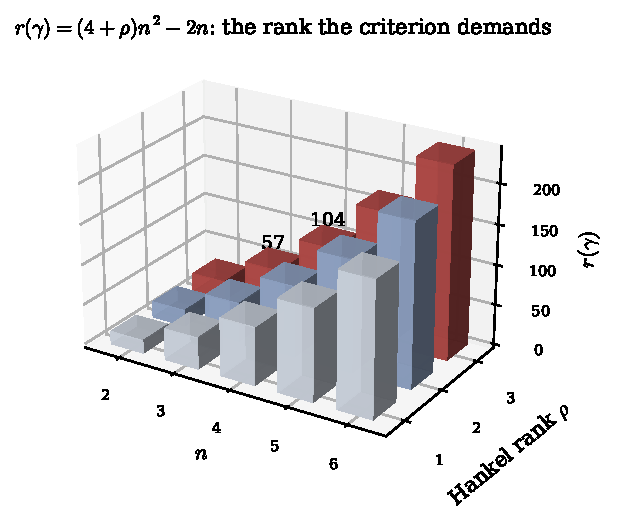
\includegraphics[width=0.78\textwidth]{figures/fig_hankel}
\caption{The lower bound $r(\gamma)=(4+\rho)n^{2}-2n$ of Theorem~\ref{thm:criterion} for $2\le n\le6$ and Hankel rank $\rho=1,2,3$. The two labelled bars are the product cases of Theorem~\ref{thm:product}.}
\label{fig:hankel}
\end{figure*}

\subsection{The Weil plane of a product}

\begin{lemma}\label{lem:weilproduct}
Let $A$, $A'$ be of Weil type for the same field $K$, of dimensions $2m$, $2m'$, with the diagonal $K$-action on $A\times A'$. Then $W(A\times A')$ is a two-dimensional rational subspace of the four-dimensional space $W(A)\otimes W(A')\subseteq H^{2n}(A\times A')$, $n=m+m'$, and every rational $w\in W(A\times A')$ is $\sum_{i,j}a_{ij}\,\omega_{i}\otimes\omega'_{j}$ with $a_{ij}\in\QQ$ for rational bases $(\omega_{i})$, $(\omega'_{j})$ of $W(A)$, $W(A')$.
\end{lemma}

\begin{proof}
Over $\CC$, $H^{1}(A\times A')=V\oplus V'$ splits into eigenspaces $V_{\pm}\oplus V'_{\pm}$ of $K$, and $\bigwedge^{2n}_{K}$ of the sum is spanned by $\det V_{+}\otimes\det V'_{+}$ and $\det V_{-}\otimes\det V'_{-}$; these lie in the span of the four products $\omega_{\pm}\otimes\omega'_{\pm}$ of the eigenvectors of $W(A)\otimes\CC$ and $W(A')\otimes\CC$. Both $W(A\times A')$ and $W(A)\otimes W(A')$ are defined over $\QQ$, so the inclusion holds over $\QQ$. The explicit formula is \cite[Eq.~(36)]{BMB26}: $\omega_{1}(A\times A')=\omega_{1}\otimes\omega'_{1}-d\,\omega_{2}\otimes\omega'_{2}$ for $K=\QQ(\sqrt{-d})$.
\end{proof}

\subsection{An object with the polarised Chern character}

\begin{theorem}[The product object]\label{thm:product}
Let $A$, $A'$ be very general in their polarised Weil families, with ample classes $\theta_{A}$, $\theta_{A'}$, $\theta=\theta_{A}+\theta_{A'}$, and suppose that $W(A)$ and $W(A')$ are algebraic. Then there is a perfect complex $\mathcal{E}$ on $A\times A'$, a finite direct sum with shifts of exterior products
\[
F_{i}\boxtimes G'_{j},\quad F_{i}\boxtimes L'^{\,k},\quad L^{l}\boxtimes G'_{j},\quad L^{l}\boxtimes L'^{\,k},
\]
with $F_{i}$, $G'_{j}$ coherent sheaves on $A$, $A'$ and $L$, $L'$ the ample bundles, such that
\[
\ch(\mathcal{E})=N\,w+\sum_{k=0}^{2n}c_{k}\theta^{k},\qquad N\ne0,\ 0\ne w\in W(A\times A'),
\]
has the polarised shape with Hankel rank $\rho=3$, so that $r(\ch\mathcal{E})=7n^{2}-2n$, and the first-order Hodge locus of $\ch(\mathcal{E})$ in $H^{1}(A\times A',T)$ is the tangent space of $\cD_{n,n}$.
\end{theorem}

The hypotheses hold in the two open cases nearest to the known ones: $A$, $A'$ very general Weil fourfolds of trivial discriminant, where Markman proves the Weil classes algebraic \cite{Mar25a,Mar25b}, so that $A\times A'$ is an eightfold with $n=4$; and $A$ such a fourfold and $A'=B$ a Weil surface of any discriminant $d$, whose Weil plane is of type $(1,1)$ and algebraic by Lefschetz, so that $A\times B$ is a sixfold of discriminant $d$ with $n=3$.

\begin{proof}
Since $\Hdg^{*}(A)=\QQ[\theta_{A}]\oplus W(A)$, algebraic classes on $A$ are rational combinations of Chern characters of coherent sheaves, and the Chern character of a coherent sheaf is a Hodge class, the algebraicity of $W(A)$ gives coherent sheaves $F_{1}$, $F_{2}$ with $\ch(F_{i})=N_{i}\omega_{i}+p_{i}(\theta_{A})$, $N_{i}\ne0$, for a basis $(\omega_{1},\omega_{2})$ of $W(A)$; likewise $G'_{1}$, $G'_{2}$ on $A'$ with $\ch(G'_{j})=N'_{j}\omega'_{j}+p'_{j}(\theta_{A'})$. Fix $0\ne w\in W(A\times A')$ rational, $w=\sum a_{ij}\omega_{i}\otimes\omega'_{j}$ by Lemma~\ref{lem:weilproduct}, and a common denominator $M$ of the numbers $Ma_{ij}/(N_{i}N'_{j})$, so that these are integers. Negative multiplicities are realised by the shift $[1]$, which changes the sign of $\ch$.

Step 1. $\mathcal{E}_{0}=\bigoplus_{i,j}(F_{i}\boxtimes G'_{j})^{\oplus Ma_{ij}/(N_{i}N'_{j})}$ has, by multiplicativity,
\begin{widetext}
\begin{equation}\label{eq:chE0}
\ch(\mathcal{E}_{0})=Mw+\sum_{i}\omega_{i}\otimes q'_{i}(\theta_{A'})+\sum_{j}q_{j}(\theta_{A})\otimes\omega'_{j}+s,
\end{equation}
\end{widetext}
with $q'_{i}$, $q_{j}$ polynomials and $s\in\QQ[\theta_{A}]\otimes\QQ[\theta_{A'}]$.

Step 2. The classes $e^{k\theta_{A'}}=\ch(L'^{\,k})$, $k=0,\dots,2m'$, form a basis of $\QQ[\theta_{A'}]/(\theta_{A'}^{2m'+1})$: the matrix $(k^{j}/j!)_{j,k}$ has determinant $\prod_{j}(1/j!)$ times the Vandermonde determinant of $0,1,\dots,2m'$, which is nonzero. Write $q'_{i}=\sum_{k}b_{ik}e^{k\theta_{A'}}$ and add $(F_{i}\boxtimes L'^{\,k})^{\oplus-Mb_{ik}/N_{i}}$, after enlarging $M$ to clear denominators; this removes $\omega_{i}\otimes q'_{i}$ and adds only terms $p_{i}(\theta_{A})\otimes e^{k\theta_{A'}}$, which lie in $\QQ[\theta_{A}]\otimes\QQ[\theta_{A'}]$. Symmetrically remove $q_{j}\otimes\omega'_{j}$ with summands $L^{l}\boxtimes G'_{j}$.

\begin{figure*}[t]
\centering
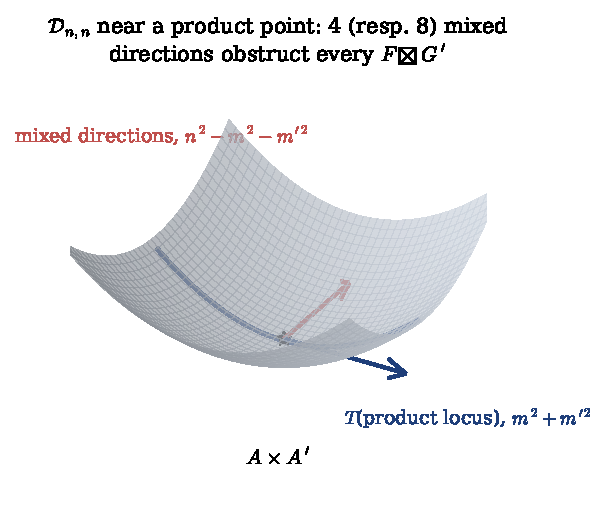
\includegraphics[width=0.78\textwidth]{figures/fig_product}
\caption{The domain $\cD_{n,n}$ near a product point $A\times A'$. The curve is the product locus, whose tangent space has dimension $m^{2}+m'^{2}$; the $2mm'$ mixed directions obstruct every exterior product $F\boxtimes G'$, and only the combined object of Theorem~\ref{thm:product} has the full tangent space as first-order Hodge locus.}
\label{fig:product}
\end{figure*}

Step 3. The classes $e^{l\theta_{A}+k\theta_{A'}}=\ch(L^{l}\boxtimes L'^{\,k})$ form a basis of $\QQ[\theta_{A}]/(\theta_{A}^{2m+1})\otimes\QQ[\theta_{A'}]/(\theta_{A'}^{2m'+1})$ by the same determinant, so the remaining part in $\QQ[\theta_{A}]\otimes\QQ[\theta_{A'}]$ is cancelled by line bundles with integer multiplicities and shifts. Finally add $(L\boxtimes L')^{\otimes k}$, $k=0,1,2$, with generic nonzero multiplicities $\mu_{k}$. The result is
\[
\ch(\mathcal{E})=Mw+\sum_{k=0}^{2}\mu_{k}e^{k\theta},
\]
a polarised shape whose polynomial part is a sum of three distinct exponentials with nonzero coefficients. Three exponentials are not one of the shapes of Hankel rank at most two, so $\rho=3$; and some $c_{k}$ with $1\le k\le2n-1$ is nonzero, so the first-order Hodge locus is the tangent space of $\cD_{n,n}$ by Theorem~\ref{thm:criterion}.
\end{proof}

The construction was carried out in the exterior-algebra model of $H^{*}(A\times A')$ for $(m,m')=(2,1)$ and $(2,2)$: the cross terms of $\ch(\mathcal{E}_{0})$ vanish, nothing is left outside $W(A\times A')\oplus\QQ[\theta]$ after Steps 2 and 3, the Hankel rank is $3$, and the first-order Hodge locus has dimension $9$, resp.\ $16$, equal to $n^{2}$ (Appendix~\ref{app:checks}).

\subsection{What a direct sum cannot do}

The tangent space of $\cD_{n,n}$ at a product point contains the tangent space of the product locus $\cD_{m,m}\times\cD_{m',m'}$, of dimension $m^{2}+m'^{2}$, and $n^{2}-m^{2}-m'^{2}=2mm'$ mixed directions. In the same model, each exterior product $F\boxtimes G'$ of sheaves of polarised shape has first-order Hodge locus inside $T\cD_{n,n}$ equal to the tangent space of the product locus: all $2mm'$ mixed directions obstruct it, four for $A\times B$ and eight for $A\times A'$ (Fig.~\ref{fig:product}). The object $\mathcal{E}$ of Theorem~\ref{thm:product} has the whole tangent space as its first-order locus because its Chern character is a single polarised class and not a product. Semiregularity is a different matter.

\begin{proposition}[Direct sums are never semiregular]\label{prop:directsum}
\leavevmode
\begin{enumerate}[label=\textup{(\roman*)},leftmargin=2.4em,itemsep=2pt]
\item Let $\mathcal{E}=\bigoplus_{k}\mathcal{E}_{k}$ be a direct sum of at least two nonzero complexes. Then the semiregularity map $\sigma_{\mathcal{E}}$ vanishes on $\bigoplus_{k\ne l}\Ext^{2}(\mathcal{E}_{k},\mathcal{E}_{l})$. So $\sigma_{\mathcal{E}}$ is injective only if $\Ext^{2}(\mathcal{E}_{k},\mathcal{E}_{l})=0$ for all $k\ne l$.
\item For every direct-sum realisation $\mathcal{E}$ of Theorem~\ref{thm:product}, $\sigma_{\mathcal{E}}$ is not injective and $\dim\Ext^{2}(\mathcal{E},\mathcal{E})>r(\ch\mathcal{E})$.
\end{enumerate}
\end{proposition}

\begin{proof}
(i) The semiregularity map of Buchweitz and Flenner is built from the traces $\xi\mapsto\mathrm{tr}\bigl(\xi\circ\mathrm{At}(\mathcal{E})^{p}\bigr)$ of compositions with powers of the Atiyah class \cite[Sect.~4]{BF03}. The Atiyah class of a direct sum is block diagonal, so for $\xi$ in an off-diagonal block $\Ext^{2}(\mathcal{E}_{k},\mathcal{E}_{l})$ the composition $\xi\circ\mathrm{At}(\mathcal{E})^{p}$ is off-diagonal, and the trace of an off-diagonal block is zero.

(ii) The summands of $\mathcal{E}$ include $F_{1}\boxtimes L'^{\,k}$ and $F_{1}\boxtimes L'^{\,l}$ for two exponents $k<l$, because Step 2 of the proof uses every power $L'^{\,k}$ with $0\le k\le2m'$ (the exponentials form a basis and $q'_{1}$ is a nonzero polynomial of positive degree for a sheaf of polarised shape, which has $p_{1}$ of positive degree by Theorem~\ref{thm:criterion}). By the K\"unneth formula
\begin{widetext}
\begin{equation}\label{eq:kunneth}
\Ext^{2}(F_{1}\boxtimes L'^{\,k},F_{1}\boxtimes L'^{\,l})\supseteq\Ext^{2}(F_{1},F_{1})\otimes H^{0}(A',L'^{\,l-k}),
\end{equation}
\end{widetext}
and $\dim\Ext^{2}(F_{1},F_{1})\ge r(\ch F_{1})\ge12$ by Theorem~\ref{thm:criterion} on the fourfold $A$ ($n=2$, $\rho\ge0$), while $H^{0}$ of an ample bundle is nonzero. So an off-diagonal block is nonzero, $\sigma_{\mathcal{E}}$ has a kernel by (i), and $\dim\Ext^{2}(\mathcal{E},\mathcal{E})>r$ because equality would force injectivity.
\end{proof}

\begin{proposition}[Convolutions]\label{prop:convolution}
Let $\mathcal{E}_{\delta}$ be a one-sided twisted complex on pieces $P_{1},\dots,P_{N}$ with shifts $s_{a}$, ordered so that the differential $\delta=(\delta_{ab})_{a<b}$, $\delta_{ab}\in\Ext^{1+s_{a}-s_{b}}(P_{a},P_{b})$, is strictly upper triangular; let $\gamma=\ch(\mathcal{E}_{\delta})=\sum_{a}(-1)^{s_{a}}\ch(P_{a})$.
\begin{enumerate}[label=\textup{(\roman*)},leftmargin=2.4em,itemsep=2pt]
\item The semiregularity map $\sigma_{\mathcal{E}_{\delta}}$ vanishes on every class of $\Ext^{2}(\mathcal{E}_{\delta},\mathcal{E}_{\delta})$ represented by a strictly upper triangular cocycle. So the criterion holds for $\mathcal{E}_{\delta}$ only if every strictly upper triangular cocycle of degree two is a coboundary.
\item Suppose no term of the twisted differential carries a class of degree one into a diagonal block $\Ext^{*}(P_{c},P_{c})$. Let $v\in T\cD_{n,n}$ have a nonzero mixed component. If some piece $P=X\boxtimes Y$ has $\operatorname{rk}Y\,c_{1}(X)/\theta_{A}\ne\operatorname{rk}X\,c_{1}(Y)/\theta_{A'}$, then $\mathrm{ev}_{\mathcal{E}_{\delta}}(v)\ne0$ and $\sigma_{\mathcal{E}_{\delta}}(\mathrm{ev}_{\mathcal{E}_{\delta}}(v))=0$: the criterion fails.
\item Suppose the pieces split into two nonempty groups with $\Ext^{*}(P_{a},P_{b})=0$ in both directions for $a$, $b$ in different groups. Then $\mathcal{E}_{\delta}=\mathcal{E}'\oplus\mathcal{E}''$ is the direct sum of the convolutions of the groups, and the criterion holds for $\mathcal{E}_{\delta}$ only if every $v\in T\cD_{n,n}$ annihilates $\ch(\mathcal{E}')$ and $\ch(\mathcal{E}'')$ separately.
\end{enumerate}
\end{proposition}

\begin{proof}
(i) The components of $\sigma_{\mathcal{E}_{\delta}}(\xi)$ are the traces $\mathrm{tr}(\xi\circ\mathrm{At}(\mathcal{E}_{\delta})^{p})/p!$ \cite[Sect.~4]{BF03}. In the harmonic model of a twisted complex the Atiyah class is represented by $[\nabla,\bar\partial+\delta]$ with $\nabla$ the direct sum of the Chern connections of the pieces; it is block upper triangular with diagonal blocks $\mathrm{At}(P_{a})$ and off-diagonal blocks $\nabla\delta_{ab}$. The homotopy transfer $\xi\mapsto\sum_{k}(-h[\delta,\,\cdot\,])^{k}\xi$ that produces the chain-level representative of $\xi$ raises or preserves the block position $b-a$, so a strictly upper triangular cocycle has a strictly upper triangular representative. The product of an upper triangular block matrix with a strictly upper triangular one is strictly upper triangular, and its trace, the sum of the traces of its diagonal blocks, is zero. The trace is a chain map for $\bar\partial+[\delta,\,\cdot\,]$ by cyclicity, so the vanishing holds in cohomology. Since $\sigma_{\mathcal{E}_{\delta}}\circ\mathrm{ev}_{\mathcal{E}_{\delta}}$ is contraction into $\gamma$, of rank $r(\gamma)$, the kernel of $\sigma_{\mathcal{E}_{\delta}}$ contains the image of the strictly upper triangular classes and $\dim\Ext^{2}\ge r(\gamma)+\dim(\text{that image})$.

(ii) The Atiyah class of $X\boxtimes Y$ is $\mathrm{At}(X)\otimes1+1\otimes\mathrm{At}(Y)$, so the diagonal component of $\mathrm{ev}_{\mathcal{E}_{\delta}}(v)$ at $P$ is $v\lrcorner\mathrm{At}(P)$, with trace $v\lrcorner\ch_{1}(P)$. Write $v=v_{A}+v_{A'}+z\otimes d'+z'\otimes d$ with $v_{A}\in T\cD_{m,m}$, $v_{A'}\in T\cD_{m',m'}$, $z\in H^{0,1}(A)$, $d'\in H^{0}(T_{A'})$, $z'\in H^{0,1}(A')$, $d\in H^{0}(T_{A})$. Since $v$ kills $\theta=\theta_{A}+\theta_{A'}$ and $v_{A}\lrcorner\theta_{A}=v_{A'}\lrcorner\theta_{A'}=0$, we have $v\lrcorner\theta_{A'}=-v\lrcorner\theta_{A}=-z'\wedge(d\lrcorner\theta_{A})$, nonzero when $d\ne0$ because $\theta_{A}$ is nondegenerate and $z'\wedge$ is injective on $H^{0,1}(A)$; the case $d=0$, $d'\ne0$ is symmetric. On a very general member $c_{1}(X)$ and $c_{1}(Y)$ are multiples of the polarisations, so $v\lrcorner\ch_{1}(P)=\bigl(\operatorname{rk}Y\,c_{1}(X)/\theta_{A}-\operatorname{rk}X\,c_{1}(Y)/\theta_{A'}\bigr)\,v\lrcorner\theta_{A}\ne0$ under the hypothesis on $P$. Under the assumption on the differential, the diagonal components of a class in $\Ext^{2}(\mathcal{E}_{\delta},\mathcal{E}_{\delta})$ are well defined, so $\mathrm{ev}_{\mathcal{E}_{\delta}}(v)\ne0$, while $\sigma_{\mathcal{E}_{\delta}}(\mathrm{ev}_{\mathcal{E}_{\delta}}(v))=v\lrcorner\gamma=0$ because $v$ is tangent to the Hodge locus of $\gamma$.

(iii) With no Ext groups between the groups there are no components of $\delta$ between them, so the twisted complex is block diagonal,
\begin{widetext}
\begin{equation}\label{eq:blockdiag}
\Ext^{2}(\mathcal{E}_{\delta},\mathcal{E}_{\delta})=\Ext^{2}(\mathcal{E}',\mathcal{E}')\oplus\Ext^{2}(\mathcal{E}'',\mathcal{E}''),\qquad
\dim\Ext^{2}(\mathcal{E}_{\delta},\mathcal{E}_{\delta})\ge\dim HT^{2}-\dim\bigl(\mathrm{Ann}(\ch\mathcal{E}')\cap\mathrm{Ann}(\ch\mathcal{E}'')\bigr),
\end{equation}
\end{widetext}
with $\sigma_{\mathcal{E}_{\delta}}=\sigma_{\mathcal{E}'}\oplus\sigma_{\mathcal{E}''}$; the inequality holds because for each summand the contraction into its Chern character factors through $\mathrm{ev}$ and $\sigma$, so that $\dim\Ext^{2}(\mathcal{E}',\mathcal{E}')$ is at least the rank of $\xi\mapsto\xi\lrcorner\ch\mathcal{E}'$, and likewise for $\mathcal{E}''$. Here $r(\gamma)=\dim HT^{2}-\dim\mathrm{Ann}(\gamma)$ with $\mathrm{Ann}(\gamma)=T\cD_{n,n}$. Equality $\dim\Ext^{2}=r(\gamma)$ forces the common annihilator to be all of $T\cD_{n,n}$.
\end{proof}

For the pieces of Theorem~\ref{thm:product} the splitting in (iii) that one would like to use separates the pieces $F_{i}\boxtimes Y$ carrying a secant sheaf on $A$ from the pieces $L^{l}\boxtimes Y'$. Two statements settle what that splitting gives. The first computes the annihilator of the secant pieces by hand; the second shows that the splitting is never available.

\begin{theorem}[The annihilator of the secant pieces]\label{thm:annihilator}
Let $\mathcal{E}'$ be the sum, with the multiplicities and shifts of Theorem~\ref{thm:product}, of the pieces $F_{i}\boxtimes G'_{j}$ and $F_{i}\boxtimes L'^{\,k}$. Then
\begin{equation}\label{eq:chEprime}
\ch(\mathcal{E}')=Mw+\sum_{i}\frac{M}{N_{i}}\,p_{i}(\theta_{A})\otimes R_{i},\qquad R_{i}=\sum_{j}a_{ij}\omega'_{j},
\end{equation}
where $(a_{ij})$ is the matrix of $w$ in the bases $(\omega_{i})$, $(\omega'_{j})$ and is invertible, and the annihilator of $\ch(\mathcal{E}')$ in $T\cD_{n,n}$ is the tangent space $T\cD_{m,m}\oplus T\cD_{m',m'}$ of the product locus, of dimension $m^{2}+m'^{2}$. If $\Ext^{*}(F_{i},L^{l})=0$ for every power $L^{l}$ among the pieces, every convolution $\mathcal{E}_{\delta}$ of the pieces has $\dim\Ext^{2}(\mathcal{E}_{\delta},\mathcal{E}_{\delta})\ge r(\gamma)+2mm'$, which is $61$ at $n=3$ and $120$ at $n=4$.
\end{theorem}

\begin{proof}
Steps 1 and 2 of Theorem~\ref{thm:product} add and subtract, for each $i$, the classes
\[
\sum_{j}\frac{Ma_{ij}}{N_{i}N'_{j}}\,\ch(F_{i})\ch(G'_{j})\quad\text{and}\quad\frac{M}{N_{i}}\,\ch(F_{i})\otimes q'_{i},
\]
where $q'_{i}=\sum_{j}(a_{ij}/N'_{j})p'_{j}$; the difference is $\ch(F_{i})\otimes R_{i}$, and summing over $i$ with $\ch(F_{i})=N_{i}\omega_{i}+p_{i}(\theta_{A})$ gives \eqref{eq:chEprime}, the terms $\omega_{i}\otimes R_{i}$ adding up to $Mw$ by the definition of $a$. By Lemma~\ref{lem:weilproduct} $w=x\,\omega_{+}\otimes\omega'_{+}+\bar x\,\omega_{-}\otimes\omega'_{-}$ with $x\ne0$, a tensor of rank two, so $a$ is invertible and $R_{1}$, $R_{2}$ form a basis of the Weil plane of $A'$.

Write $V=H^{1}(A,\CC)=V_{+}\oplus V_{-}$ for the eigenspaces of $K$, $\omega_{\pm}=\det V_{\pm}$, and $V'_{\pm}$, $\omega'_{\pm}$ for their analogues on $A'$. A tangent vector $v\in H^{1}(T_{A\times A'})$ acts on cohomology as a derivation and decomposes as $v=v_{A}+v_{A'}+\mu+\mu'$ with $v_{A}\in H^{0,1}(A)\otimes H^{0}(T_{A})$, $v_{A'}$ its analogue on $A'$, and the mixed parts $\mu\in H^{0,1}(A)\otimes H^{0}(T_{A'})$, $\mu'\in H^{0,1}(A')\otimes H^{0}(T_{A})$. Let $v\in T\cD_{n,n}$. The three K\"unneth components of $v\lrcorner\theta$ vanish separately: $v_{A}\lrcorner\theta_{A}=0$, $v_{A'}\lrcorner\theta'=0$ and $\mu\lrcorner\theta'+\mu'\lrcorner\theta_{A}=0$. Contraction into a nondegenerate form is an isomorphism from $H^{0}(T)$ onto $H^{0,1}$, so $\mu\mapsto\mu\lrcorner\theta'$ and $\mu'\mapsto\mu'\lrcorner\theta_{A}$ are injective into $H^{0,1}(A)\otimes H^{0,1}(A')$, and $\mu=0$ exactly when $\mu'=0$. Next, $v\lrcorner(\omega_{+}\otimes\omega'_{+})=0$. The term $(v_{A}\lrcorner\omega_{+})\otimes\omega'_{+}$ has no component in $\Lambda^{2m}V_{+}\otimes\Lambda^{2m'}V'_{+}$, because that component is the trace of $v_{A}$ on $V_{+}$ and $v_{A}$ sends $V_{+}^{1,0}$ into $V_{+}^{0,1}$ and kills $V_{+}^{0,1}$; it lies in $\Lambda^{2m-1}V_{+}\otimes V_{-}\otimes\Lambda^{2m'}V'_{+}$, while the other three terms lie in $\Lambda^{2m}V_{+}\otimes\Lambda^{2m'-1}V'_{+}\otimes V'_{-}$, in $\Lambda^{2m-1}V_{+}\otimes\Lambda^{2m'}V'_{+}\otimes V'_{-}$ and in $\Lambda^{2m}V_{+}\otimes V_{-}\otimes\Lambda^{2m'-1}V'_{+}$, four distinct weight spaces for $GL(V_{+})\times GL(V_{-})\times GL(V'_{+})\times GL(V'_{-})$. Hence $v_{A}\lrcorner\omega_{+}=0$, and in the same way $v_{A}\lrcorner\omega_{-}=0$ and $v_{A'}\lrcorner\omega'_{\pm}=0$. A vector of $T\cD_{n,n}$ with vanishing mixed part therefore lies in $T\cD_{m,m}\oplus T\cD_{m',m'}$, and conversely every such sum kills $\theta$ and the Weil plane; the dimension $m^{2}+m'^{2}$ is that of the two Weil families \cite{Weil77}.

Now let $v\in T\cD_{n,n}$ have $\mu\ne0$. It kills $Mw$; $v_{A}$ kills $p_{i}(\theta_{A})$ and $v_{A'}$ kills $R_{i}$; so $v\lrcorner\ch(\mathcal{E}')=(\mu+\mu')\lrcorner\sum_{k}\theta_{A}^{k}\otimes R^{(k)}$, where $p_{i}=\sum_{k}c_{ik}\theta_{A}^{k}$ and $R^{(k)}=\sum_{i}(Mc_{ik}/N_{i})R_{i}$. Write $\mu=\sum_{s}z_{s}\otimes d'_{s}$ and $\mu'=\sum_{s}z'_{s}\otimes d_{s}$. The contraction of $\theta_{A}^{k}\otimes R^{(k)}$ against $\mu'$ is $k\sum_{s}\theta_{A}^{k-1}(d_{s}\lrcorner\theta_{A})\otimes(z'_{s}\wedge R^{(k)})$, of K\"unneth bidegree $(2k-1,2m'+1)$, and against $\mu$ it is $\sum_{s}(z_{s}\wedge\theta_{A}^{k})\otimes(d'_{s}\lrcorner R^{(k)})$, of bidegree $(2k+1,2m'-1)$. These bidegrees are pairwise distinct over all $k$ and both types, so every term vanishes on its own. Some $R^{(k)}$ is nonzero, since $p_{1}$, $p_{2}$ are not both zero and $R_{1}$, $R_{2}$ are a basis. For $R=\sigma\omega'_{+}+\bar\sigma\omega'_{-}$ with $\sigma\ne0$ the map $z'\mapsto z'\wedge R$ is injective on $H^{0,1}(A')$, because $z'\wedge\omega'_{+}=z'_{-}\wedge\omega'_{+}$ and $z'\wedge\omega'_{-}=z'_{+}\wedge\omega'_{-}$ lie in independent weight spaces and vanish only with $z'_{\mp}$; dually $d'\mapsto d'\lrcorner R$ is injective on $H^{0}(T_{A'})$. If the nonzero $R^{(k)}$ has $k\ge1$, hard Lefschetz makes $\theta_{A}^{k-1}$ injective on $H^{1}(A)$, since $k-1\le2m-1$, so the $\mu'$-term vanishes only if $\sum_{s}(d_{s}\lrcorner\theta_{A})\otimes z'_{s}=0$, that is $\mu'=0$, and then $\mu=0$. If $k=0$ the $\mu$-term is $(\mathrm{id}\otimes(\,\cdot\,\lrcorner R^{(0)}))(\mu)$, which vanishes only if $\mu=0$. Either way the mixed part is zero, against the assumption.

The bound is Proposition~\ref{prop:convolution}(iii): the common annihilator of $\ch\mathcal{E}'$ and $\ch\mathcal{E}''$ in $T\cD_{n,n}$ lies in that of $\ch\mathcal{E}'$, so $\dim\Ext^{2}\ge\dim HT^{2}-m^{2}-m'^{2}=r(\gamma)+n^{2}-m^{2}-m'^{2}$, and $n=m+m'$.
\end{proof}

\begin{proposition}[Secant and line-bundle pieces are never orthogonal]\label{prop:noorth}
For every realisation of Theorem~\ref{thm:product} there are an index $i$ and a power $L^{l}$ among the pieces with $\chi(F_{i},L^{l})\ne0$. Hence $\Ext^{*}(F_{i},L^{l})\ne0$ and $\Ext^{*}(L^{l},F_{i})\ne0$, and the hypothesis of the last sentence of Theorem~\ref{thm:annihilator} fails.
\end{proposition}

\begin{proof}
The Todd class of $A$ is $1$, $\omega_{i}\theta_{A}=0$ and $\int\theta_{A}^{4}=24$, so Riemann--Roch gives $\chi(F_{i},L^{l})=\int p_{i}(-\theta_{A})e^{l\theta_{A}}=P_{i}(l)$ with
\begin{equation}\label{eq:rrpoly}
P_{i}(l)=c_{i0}l^{4}-4c_{i1}l^{3}+12c_{i2}l^{2}-24c_{i3}l+24c_{i4},
\end{equation}
a nonzero polynomial because $p_{i}\ne0$. Expand $p_{i}=\sum_{l}b_{il}e^{l\theta_{A}}$, $0\le l\le4$, modulo $\theta_{A}^{5}$, which is possible since the five exponentials span $\QQ[\theta_{A}]/(\theta_{A}^{5})$, and call the set $S_{i}$ of $l$ with $b_{il}\ne0$ the support of $p_{i}$. Then $P_{i}(s)=\sum_{l\in S_{i}}b_{il}(s-l)^{4}$. If $P_{i}$ vanished on all of $S_{i}$ with $|S_{i}|\ge2$, the vector $(b_{il})_{l\in S_{i}}$ would lie in the kernel of the symmetric matrix $\bigl((s-l)^{4}\bigr)_{s,l\in S_{i}}$. That matrix is nonsingular: for two elements its determinant is $-(s-l)^{8}$, for three it is $2\prod(s-l)^{4}$, for the five four-element subsets of $\{0,\dots,4\}$ it is $29952$, $1032192$, $6054912$, $1032192$, $29952$, and for the whole set it is $7962624$. So a support with at least two elements contains some $l$ with $P_{i}(l)\ne0$.

Step~2 of Theorem~\ref{thm:product} uses the pieces $L^{l}\boxtimes G'_{j}$ for every $l$ in the support of $q_{j}=\sum_{i}(Ma_{ij}/N_{i})p_{i}$, and the last step uses $L^{k}\boxtimes L'^{\,k}$ for three values of $k$ whose net multiplicities are nonzero. If $p_{1}$ and $p_{2}$ are independent, $q_{1}$ and $q_{2}$ span the same plane because $a$ is invertible, so the union of their supports is $S_{1}\cup S_{2}$; if $p_{2}$ is a multiple of $p_{1}$, both $q_{j}$ are multiples of $p_{1}$, not both zero, with the same support. In either case every $l\in S_{1}\cup S_{2}$ gives a piece $L^{l}\boxtimes G'_{j}$. If $|S_{1}|\ge2$ or $|S_{2}|\ge2$ we are done. Otherwise $p_{i}=b_{i}e^{l_{i}\theta_{A}}$ with $b_{i}\ne0$. If $l_{1}\ne l_{2}$ then $L^{l_{2}}\boxtimes G'_{j}$ is a piece and $P_{1}(l_{2})=b_{1}(l_{2}-l_{1})^{4}\ne0$. If $l_{1}=l_{2}=l$ the residue of Steps 1 to 3 lies in $e^{l\theta_{A}}\otimes\QQ[\theta']$, so at least two of the three final exponents $k$ differ from $l$, and $P_{i}(k)=b_{i}(k-l)^{4}\ne0$. The vanishing of $\Ext^{*}(F_{i},L^{l})$ would force $\chi(F_{i},L^{l})=0$; Serre duality gives $\Ext^{*}(L^{l},F_{i})\ne0$ as well.
\end{proof}

Theorem~\ref{thm:annihilator} is therefore a conditional statement whose condition never holds: Proposition~\ref{prop:convolution}(iii) cannot be applied to the splitting between secant pieces and line-bundle pieces, and no bound on $\dim\Ext^{2}$ of a convolution follows from the Chern characters alone. The hypothesis of part (ii) can fail with line bundles only. The cone of a section of $L^{l}\boxtimes L'^{\,k'-k}$, viewed as a map $L^{l}\boxtimes L'^{\,k}\to L^{l}\boxtimes L'^{\,k'}$ with $k'>k$, is a twisted complex of two pieces in which the Serre dual of the section, a class of degree one, enters the diagonal block of the piece $L^{l}\boxtimes L'^{\,k}$; the only terms that can enter a diagonal block of a line-bundle piece are of this form, with the same power on $A$. Part (ii) applies to every piece $L^{l}\boxtimes L'^{\,k}$ with $l\ne k$ whose block receives no such term, which is how Step~3 of Theorem~\ref{thm:product} uses it.

\subsection{Where the product object stops}\label{ssec:f2stop1}

Every test that depends on $\ch(\mathcal{E})$ alone is passed: polarised shape, $N\ne0$, Hankel rank $3$, first-order Hodge locus equal to $T\cD_{n,n}$, lower bound $57$ or $104$. The criterion then asks for $\dim\Ext^{2}(\mathcal{E},\mathcal{E})=r$, Proposition~\ref{prop:directsum} shows that no direct sum achieves it, and Proposition~\ref{prop:convolution} says what a convolution of the same pieces must do: kill every strictly upper triangular class of degree two, carry classes of degree one from the lower triangle into the diagonal blocks of every piece with mismatched slopes, and, since by Proposition~\ref{prop:noorth} the secant pieces and the line-bundle pieces are never orthogonal, carry classes between the two groups in a way that cancels the mixed directions, which by Theorem~\ref{thm:annihilator} the secant pieces alone leave uncancelled. All three demands are statements about the groups $\Ext^{*}(F_{1},F_{2})$, $\Ext^{*}(F_{i},L^{l})$, $\Ext^{*}(L^{l},F_{i})$ and their analogues on $A'$. Those groups are not computed in \cite{Mar25a,Mar25b,Mar25c}, where the only object with known Ext groups on a very general Weil fourfold of trivial discriminant is the twisted transform $\Phi(F\boxtimes F^{\vee})$ with $\dim\Ext^{k}=1,8,18,8,1$, whose Brauer class is half the Poincar\'e class and which therefore cannot be mixed with untwisted line bundles; and we have not computed them. Riemann--Roch fixes $\chi(F_{i},L^{l})=P_{i}(l)$ and the K\"unneth formula fixes everything on the line-bundle side, so the unknown is exactly the thirteen graded groups $\Ext^{*}(F_{i},F_{j})$ and $\Ext^{*}(F_{i},L^{l})$. This is the exact stopping point: the polarised criterion at a product point is a finite question about the Ext algebra of the secant sheaves, and Proposition~\ref{prop:convolution} lists what the answer must contain for the route to stay open. The analogous question on $E_{0}^{6}$, for line bundles, closed negatively with $\dim\Ext^{2}\ge69$ \cite[Thm.~18.35]{BMB26}; that is an analogy and not a proof of the answer here.

At a point of complex multiplication the thirteen groups are known. We record them, since they turn the stopping point into a statement about one explicit variety.

\begin{lemma}[The Ext groups at a point of complex multiplication]\label{lem:cmext}
Let $K=\QQ(i)$, $E_{0}=\CC/\ZZ[i]$, and let $A_{0}=E_{0}^{6}$ carry the $K$-action by $i$ on three factors and by $-i$ on the other three; it is a member of $\cD_{3,3}$ for every discriminant, since the $K$-hermitian forms $\sum_{j\le3}a_{j}z_{j}\bar w_{j}-\sum_{j>3}a_{j}z_{j}\bar w_{j}$ with $a_{j}>0$ are polarisations of every discriminant class. Let $L$ be ample on $A_{0}$ with class $\theta$, let $Z,Z'\subseteq A_{0}$ be abelian subvarieties of dimension three with $Z\cap Z'$ finite, and put $\chi_{Z}=(\theta|_{Z})^{3}/6$, a positive integer.
\begin{enumerate}[label=\textup{(\roman*)},leftmargin=2.4em,itemsep=2pt]
\item Every Hodge class on $A_{0}$ is a polynomial in divisor classes, and every product of three divisor classes is a rational combination of classes $[Z]$ of abelian threefolds. The Weil classes are such combinations, and no Weil class is a multiple of a single $[Z]$. For every $Z$, $\ch(\mathcal{O}_{Z})=[Z]$ and $\ch(\mathcal{O}_{Z}\otimes L^{a})=[Z]\,e^{a\theta}$.
\item $\Ext^{k}(\mathcal{O}_{Z}\otimes L^{a},\mathcal{O}_{Z'}\otimes L^{b})=0$ for $k\ne3$, and $\dim\Ext^{3}=|Z\cap Z'|=(Z\cdot Z')$, for all $a,b$.
\item The groups $\Ext^{k}(\mathcal{O}_{Z}\otimes L^{a},\mathcal{O}_{Z}\otimes L^{b})$ are given by \eqref{eq:cmextz} below, with $N_{Z}\cong\mathcal{O}_{Z}^{3}$. For $a=b$ it has dimension $\binom{6}{k}$ and the characteristic map $HT^{2}(A_{0})\to\Ext^{2}$ is onto; for $b>a$ it lives in degrees $0$ to $3$, of dimension $\binom{3}{k}(b-a)^{3}\chi_{Z}$; for $b<a$ in degrees $3$ to $6$, of dimension $\binom{3}{k-3}(a-b)^{3}\chi_{Z}$.
\item For $b>a$, $\Ext^{k}(\mathcal{O}_{Z}\otimes L^{a},L^{b})$ is concentrated in degree $3$ and $\Ext^{k}(L^{a},\mathcal{O}_{Z}\otimes L^{b})$ in degree $0$, both of dimension $(b-a)^{3}\chi_{Z}$; for $b<a$ the first is concentrated in degree $6$ and the second in degree $3$, both of dimension $(a-b)^{3}\chi_{Z}$; for $a=b$ the dimensions are $\binom{3}{k-3}$ and $\binom{3}{k}$.
\item For $b>a$, $\Ext^{k}(L^{a},L^{b})=H^{k}(A_{0},L^{b-a})$ is concentrated in degree $0$, of dimension $(b-a)^{6}\theta^{6}/720$; for $b<a$ in degree $6$; for $a=b$ it is $H^{k}(\mathcal{O}_{A_{0}})$, of dimension $\binom{6}{k}$.
\end{enumerate}
\end{lemma}

\begin{proof}
(i) The Hodge group of $A_{0}$ is the norm-one torus $K^{1}$ acting by $z$ on $V_{+}$ and $\bar z$ on $V_{-}$, so over $\CC$ the Hodge classes of degree $2k$ are $\bigwedge^{k}V_{+}\otimes\bigwedge^{k}V_{-}$, which is spanned by the products of $k$ elements of $V_{+}\otimes V_{-}=\Hdg^{2}(A_{0})_{\CC}$; since $\Hdg^{2}=\NS_{\QQ}$ by Lefschetz, the $\QQ$-span of the products of $k$ divisor classes has full dimension $\binom{6}{k}^{2}$. The classes $f^{*}[0]$, $f\in\Hom(E_{0}^{6},E_{0})=\ZZ[i]^{6}$, are the rank-one hermitian forms $v\bar v^{\mathsf{T}}$ and span $\NS_{\QQ}$. For $f_{1},f_{2},f_{3}$ independent over $K$ the map $f=(f_{1},f_{2},f_{3})\colon A_{0}\to E_{0}^{3}$ is a surjective homomorphism, hence flat, and $f_{1}^{*}[0]\,f_{2}^{*}[0]\,f_{3}^{*}[0]=f^{*}[0]=[f^{-1}(0)]$ is a positive multiple of the class of the abelian threefold $\ker(f)^{\circ}$; for dependent $f_{i}$ the product is zero. A Weil class $w$ satisfies $w\theta=0$, while $[Z]\theta=i_{*}(\theta|_{Z})\ne0$ because $(\theta|_{Z})^{3}>0$. Since $Z$ is a translate of a subgroup, $N_{Z}$ is trivial and $\mathrm{td}(N_{Z})=1$, so Grothendieck--Riemann--Roch gives $\ch(i_{*}\mathcal{O}_{Z})=i_{*}(1)=[Z]$ and $\ch(\mathcal{O}_{Z}\otimes L^{a})=[Z]e^{a\theta}$.

(ii) Since $\dim Z\cap Z'=0$ and the tangent spaces are translation invariant, $T_{Z}\oplus T_{Z'}=T_{A_{0}}$ at every point of $Z\cap Z'$, so $Z$ and $Z'$ are locally transverse complete intersections and $Z\cap Z'$ is reduced. In local coordinates with $Z=\{x_{1}=x_{2}=x_{3}=0\}$ and $Z'=\{y_{1}=y_{2}=y_{3}=0\}$, the Koszul resolution of $\mathcal{O}_{Z}$ gives $\mathcal{E}xt^{k}(\mathcal{O}_{Z},\mathcal{O}_{Z'})$ as the cohomology of the Koszul complex of $x_{1},x_{2},x_{3}$ on $\mathcal{O}_{Z'}$, a regular sequence there; so $\mathcal{E}xt^{k}=0$ for $k\ne3$ and $\mathcal{E}xt^{3}=\mathcal{O}_{Z\cap Z'}$. The local-to-global spectral sequence has one row, $H^{k-3}(Z\cap Z',\mathcal{O})$, and twisting by line bundles does not change a sheaf on a finite reduced scheme; the intersection number equals $|Z\cap Z'|$ by transversality.

(iii) Let $\pi\colon A_{0}\to A_{0}/Z$ be the quotient. The normal bundle $N_{Z}$ is the restriction of the trivial bundle $\pi^{*}T_{A_{0}/Z}$, so it extends to all of $A_{0}$, and by the theorem of Arinkin and C\u{a}ld\u{a}raru \cite{AC12} the derived restriction $i^{*}i_{*}\mathcal{O}_{Z}$ is formal, $i^{*}i_{*}\mathcal{O}_{Z}\cong\bigoplus_{p}\bigwedge^{p}N_{Z}^{\vee}[p]$. Hence
\begin{widetext}
\begin{equation}\label{eq:cmextz}
\Ext^{k}(\mathcal{O}_{Z}\otimes L^{a},\mathcal{O}_{Z}\otimes L^{b})=\Ext^{k}_{Z}\bigl(i^{*}i_{*}\mathcal{O}_{Z},L^{b-a}|_{Z}\bigr)=\bigoplus_{p+q=k}H^{q}\bigl(Z,L^{b-a}|_{Z}\bigr)\otimes\textstyle\bigwedge^{p}N_{Z}.
\end{equation}
\end{widetext}
For $a=b$ the dimension is $\sum_{p+q=k}\binom{3}{q}\binom{3}{p}=\binom{6}{k}$; for $b\ne a$ the cohomology of $L^{b-a}|_{Z}$ on the abelian threefold $Z$ sits in degree $0$ or $3$ according to the sign of $b-a$, with dimension $|b-a|^{3}\chi_{Z}$ by Riemann--Roch, which gives the two ranges of degrees and their dimensions. The characteristic map sends $H^{2}(\mathcal{O}_{A_{0}})$ onto $H^{2}(\mathcal{O}_{Z})$ by restriction, $H^{1}(T_{A_{0}})=H^{1}(\mathcal{O})\otimes T_{0}$ onto $H^{1}(\mathcal{O}_{Z})\otimes N_{Z,0}$ through the quotient $T_{0}\to N_{Z,0}$, and $H^{0}(\bigwedge^{2}T_{A_{0}})=\bigwedge^{2}T_{0}$ onto $\bigwedge^{2}N_{Z,0}$; all three are surjective, the first because $H^{*}(A_{0})\to H^{*}(Z)$ is onto for an abelian subvariety.

(iv) By Grothendieck duality for the regular embedding, whose relative dualising sheaf $\det N_{Z}$ is trivial, and by adjunction,
\begin{align*}
\Ext^{k}(\mathcal{O}_{Z}\otimes L^{a},L^{b})&=H^{k-3}\bigl(Z,L^{b-a}|_{Z}\bigr),\\
\Ext^{k}(L^{a},\mathcal{O}_{Z}\otimes L^{b})&=H^{k}\bigl(Z,L^{b-a}|_{Z}\bigr).
\end{align*}
On $Z$ the cohomology of an ample bundle is concentrated in degree $0$ and that of an anti-ample one in degree $3$, of dimension $\chi=c_{1}^{3}/6$ by Riemann--Roch, and $c_{1}(L^{m}|_{Z})^{3}=m^{3}(\theta|_{Z})^{3}$; for $m=0$ one gets $H^{*}(\mathcal{O}_{Z})$.

(v) is the same statement on $A_{0}$, with $\chi(L^{m})=m^{6}\theta^{6}/720$.
\end{proof}

\begin{lemma}[Threefolds that meet along a positive-dimensional set]\label{lem:cmmeet}
Let $Z,Z'\subseteq A_{0}$ be distinct abelian threefolds, let $W=Z\cap Z'$, of dimension $d\in\{0,1,2\}$, and put $c=3-d$ and $m=b-a$.
\begin{enumerate}[label=\textup{(\roman*)},leftmargin=2.4em,itemsep=2pt]
\item $\mathcal{H}om(\mathcal{O}_{Z},\mathcal{O}_{Z'})=0$, and $\mathcal{E}xt^{q}(\mathcal{O}_{Z},\mathcal{O}_{Z'})\cong\mathcal{O}_{W}^{\binom{d}{q-c}}$ for $c\le q\le3$, zero otherwise.
\item $\Ext^{k}(\mathcal{O}_{Z}\otimes L^{a},\mathcal{O}_{Z'}\otimes L^{b})=0$ unless $c\le k\le3$ when $m>0$, $3\le k\le3+d$ when $m<0$, and $c\le k\le3+d$ when $m=0$. In particular the group vanishes in degrees $k\le2$ when $m<0$, and $\Ext^{1}\ne0$ only when $d=2$ and $m\ge0$, where $\Ext^{1}=H^{0}(W,L^{m}|_{W})$.
\item For the threefolds $Z_{\zeta}$, $Z_{\zeta'}$ of Appendix~\ref{app:cmpoint}, $d$ is the number of indices $j$ with $\zeta_{j}=\zeta'_{j}$, $W$ is the product of the shared curves with $\prod_{\zeta_{j}\ne\zeta'_{j}}|\zeta_{j}-\zeta'_{j}|^{2}$ points, and for $d=2$ and $m=0$, $\dim\Ext^{1}=|\zeta_{l}-\zeta'_{l}|^{2}\in\{2,4\}$, $l$ being the index at which they differ.
\end{enumerate}
\end{lemma}

\begin{proof}
(i) $W$ is a closed subgroup scheme of $A_{0}$, reduced in characteristic zero, so a disjoint union of translates of an abelian variety of dimension $d$, and it is nonempty since $Z$ and $Z'$ contain the origin. At a point of $W$ choose translation-invariant linear coordinates in which $Z=\{x_{1}=x_{2}=x_{3}=0\}$. The restrictions of $x_{1},x_{2},x_{3}$ to $Z'$ are linear forms cutting out $W$, of codimension $c$ in $Z'$; after a linear change $x_{1},\dots,x_{c}$ restrict to a regular sequence on $Z'$ with zero locus $W$ and $x_{c+1},\dots,x_{3}$ restrict to zero. The Koszul resolution of $\mathcal{O}_{Z}$ computes $\mathcal{E}xt^{q}(\mathcal{O}_{Z},\mathcal{O}_{Z'})$ as the cohomology of the Koszul complex of these restrictions on $\mathcal{O}_{Z'}$, the tensor product of the Koszul complex of the regular sequence, with cohomology $\mathcal{O}_{W}$ in degree $c$, and of $d$ complexes $\mathcal{O}_{Z'}\xrightarrow{0}\mathcal{O}_{Z'}$; so $\mathcal{E}xt^{q}=\bigwedge^{q-c}(\mathcal{O}_{W}^{d})$. Since $c\ge1$, $\mathcal{H}om=0$.

(ii) The local-to-global spectral sequence has $E_{2}^{p,q}=H^{p}(W,\mathcal{E}xt^{q}\otimes L^{m}|_{W})$ with $0\le p\le d$ and $c\le q\le3$. On each component of $W$ the bundle $L^{m}|_{W}$ is ample for $m>0$, with cohomology in degree $0$ only, anti-ample for $m<0$, with cohomology in degree $d$ only, and trivial for $m=0$. This gives the three ranges. For $k=1$ the only possible term is $E_{2}^{0,1}$, nonzero only when $c=1$ and $m\ge0$, and it survives to $E_{\infty}$ because $E_{2}^{1,0}=E_{2}^{2,0}=0$.

(iii) In the coordinates of Appendix~\ref{app:cmpoint}, $Z_{\zeta}=\{u_{j}+\zeta_{j}v_{j}=0,\ j=1,2,3\}$; a shared index gives a form vanishing on $Z_{\zeta'}$, and an index with $\zeta_{j}\ne\zeta'_{j}$ gives the form $(\zeta_{j}-\zeta'_{j})v_{j}$ on $Z_{\zeta'}$, whose zero locus in $C_{\zeta'_{j}}$ has $|\zeta_{j}-\zeta'_{j}|^{2}$ points by Lemma~\ref{lem:cmcurves}(ii). So $W$ is as stated, and $\Ext^{1}=H^{0}(W,\mathcal{O}_{W})$ has dimension the number of components of $W$.
\end{proof}

Theorem~\ref{thm:criterion} applies at $A_{0}$ with the same number $r=57$: the rank of the contraction of $HT^{2}$ into $\ch(\mathcal{E})$ is invariant under $\SU(V,H)(\RR)$, which fixes the Weil classes and $\theta$ and acts transitively on $\cD_{3,3}$, so it is the rank computed at a very general point, and the argument of Buchweitz and Flenner is local on the base. An object $\mathcal{E}$ with $\dim\Ext^{2}(\mathcal{E},\mathcal{E})=57$ at $A_{0}$ would therefore deform along all of $\cD_{3,3}$ and prove the Weil classes algebraic on every member with full Hodge group. By (i) every Chern character of polarised shape is realised at $A_{0}$ by a convolution of pieces $\mathcal{O}_{Z_{a}}\otimes L^{k_{a}}[s_{a}]$ and $L^{k}[t]$, with at least two subvariety pieces, since $w$ is not a multiple of one $[Z]$, and at least three powers of $L$, since the Hankel rank is three; by (ii) to (v) every group between two pieces is known. Appendix~\ref{app:cmpoint} writes the classes, the intersection numbers and every dimension of the lemma in coordinates for the threefolds that are products of elliptic curves of the three Weil surfaces, and exhibits the signed sum of thirty-two of them equal to $32(\alpha+\bar\alpha)$. What the lemma decides is how the diagonal classes can disappear.

\begin{proposition}[No cancellation in two steps]\label{prop:twostep}
Let $\mathcal{E}$ be a convolution of pieces $F_{a}[s_{a}]$ of the types of Lemma~\ref{lem:cmext}, whose threefolds meet pairwise in finite sets, and no two of which are isomorphic sheaves placed at shifts differing by at most one. A class of $\Ext^{2}(F_{a},F_{a})$ is cancelled in the spectral sequence of the convolution only through a closed chain $a=a_{0},a_{1},\dots,a_{m}=a$ of pieces with $\Ext^{k_{i}}(F_{a_{i-1}},F_{a_{i}})\ne0$ and $\sum_{i}k_{i}=m$, and no such chain has $m=2$. The chains with $m=3$ are exactly those through three twists $k<k'<k''$ of one threefold, $\mathcal{O}_{Z}\otimes L^{k}[s]\to\mathcal{O}_{Z}\otimes L^{k'}[s+1]\to\mathcal{O}_{Z}\otimes L^{k''}[s+2]\to\mathcal{O}_{Z}\otimes L^{k}[s]$, with degrees $0,0,3$. Hence every cancellation among the diagonal classes of degree two is a Massey product of length at least three.
\end{proposition}

\begin{proof}
The Maurer--Cartan components of the twisted complex and the class $\eta$ whose differential is computed all have total degree one, that is, a component in $\Ext^{k}(F_{a},F_{b})$ has $k+s_{b}-s_{a}=1$. A product of $m$ such components along a closed chain lands in $\Ext^{\sum k_{i}-m+2}(F_{a},F_{a})$, since the shifts cancel around the chain and the $m$-fold product lowers the degree by $m-2$; so it reaches degree two exactly when $\sum k_{i}=m$. For $m=2$ both components have degree at most two. Between two pieces that are not isomorphic sheaves, Lemma~\ref{lem:cmext} gives the degrees: $3$ and $3$ between $\mathcal{O}_{Z}$ and $\mathcal{O}_{Z'}$; $0$ to $3$ one way and $3$ to $6$ the other between two twists of one $\mathcal{O}_{Z}$; $3$ and $3$ between $\mathcal{O}_{Z}\otimes L^{a}$ and $L^{b}$ with $a<b$, $6$ and $0$ with $a>b$, and $3$ to $6$ against $0$ to $3$ for $a=b$; $0$ and $6$ between two powers of $L$. In every case the two degrees add up to at least three. Between two copies of one sheaf at shifts $s$, $s'$ the two degrees are $1-s'+s$ and $1-s+s'$, which are both at most two only when $|s-s'|\le1$, the case excluded. For $m=3$ the edges of degree at most two are, by the same list, the edges that raise the twist and the edges $L^{a}\to\mathcal{O}_{Z}\otimes L^{a}$; a closed chain cannot consist of them alone, so one edge has degree at least three and the other two have degree zero. Two edges of degree zero from a line bundle lead to a power of $L$ or to a subvariety piece of strictly larger twist, from which every edge back to the line bundle has degree six; from $\mathcal{O}_{Z}\otimes L^{k}$ they lead only to $\mathcal{O}_{Z}\otimes L^{k''}$ with $k''>k$ through an intermediate twist $k'$, and the edge back has degree three, through $H^{3}(Z,L^{k-k''}|_{Z})\otimes\bigwedge^{0}N_{Z}$. These are the chains displayed, and their three groups are nonzero.

\end{proof}

For line-bundle pieces alone the same bookkeeping holds on $E_{0}^{6}$, and there the Massey products of length four are the ones that act, with the result $\dim\Ext^{2}\ge69$ \cite[Thm.~18.35]{BMB26}. With subvariety pieces and three powers of $L$ no closed chain of any length exists, and the criterion fails for a reason that involves no product at all.

\begin{proposition}[Convolutions with three line bundles fail]\label{prop:separated}
Let $\mathcal{E}$ be a convolution at $A_{0}$ of pieces $\mathcal{O}_{Z_{a}}\otimes L^{k_{a}}[s_{a}]$ and $L^{l_{b}}[t_{b}]$ in which no sheaf occurs twice, the threefolds $Z_{a}$ are pairwise distinct, there are at most three line bundles, and $\Ext^{1}(\mathcal{O}_{Z_{a}}\otimes L^{k_{a}},\mathcal{O}_{Z_{b}}\otimes L^{k_{b}})=0$ whenever $s_{a}=s_{b}$. Suppose $\ch(\mathcal{E})$ has the polarised shape. Then no term of the twisted differential carries a class of total degree one into a diagonal block, and
\[
\dim\Ext^{2}(\mathcal{E},\mathcal{E})\ >\ r(\ch\mathcal{E}):
\]
the criterion fails for $\mathcal{E}$. The hypothesis on $\Ext^{1}$ holds when the threefolds meet pairwise in finite sets, and for the thirty-two threefolds $Z_{\zeta}$ of Appendix~\ref{app:cmpoint} placed at one twist with shifts of the parity of $\zeta_{1}\zeta_{2}\zeta_{3}$.
\end{proposition}

\begin{proof}
Step 1, no closed chain. As in the proof of Proposition~\ref{prop:twostep}, a term of the differential landing in a diagonal block runs along a closed chain $a_{0},a_{1},\dots,a_{m}=a_{0}$ of pieces with a nonzero component in $\Ext^{k_{i}}(F_{a_{i-1}},F_{a_{i}})$, $k_{i}=1+s_{a_{i-1}}-s_{a_{i}}$, so that $\sum_{i}k_{i}=m$; the pieces of the chain are distinct, because the differential is strictly upper triangular in the one-sided order. We show that no such chain exists. Between two distinct threefold pieces $\Hom=0$ by Lemma~\ref{lem:cmmeet}(i), and a component of degree one needs $s_{a}=s_{b}$, which the hypothesis excludes; so every edge between two threefold pieces has degree at least two. By Lemma~\ref{lem:cmext}(iv) and (v), an edge $L^{l}\to\mathcal{O}_{Z}\otimes L^{k}$ has degree $0$ when $k>l$, $3$ when $k<l$ and $0$ to $3$ when $k=l$, so a degree at most one forces $k\ge l$; an edge $\mathcal{O}_{Z}\otimes L^{k}\to L^{l}$ has degree $3$ when $l>k$, $6$ when $l<k$ and $3$ to $6$ when $l=k$, so a degree at most four forces $l\ge k$; and an edge between two line bundles has degree $0$ when it raises the twist and $6$ when it lowers it. A chain of threefold pieces alone has $\sum_{i}k_{i}\ge2m>m$. Otherwise the chain visits $\ell\le3$ line-bundle pieces; between consecutive visits it either passes directly, by an edge that raises the twist ($u$ such edges in all) or lowers it ($w$ in all), or runs through $r\ge1$ threefold pieces, entered with degree $e$ and left with degree $x$; let $R$ be the number of runs. Then $R+u+w=\ell$, $m=\ell+\sum_{\mathrm{runs}}r$, a run contributes at least $e+x+2(r-1)$ to $\sum_{i}k_{i}$, and so
\[
\sum_{i}k_{i}-m\ \ge\ \sum_{\mathrm{runs}}\bigl(e+x+r-3\bigr)+5w-u ,
\]
where each bracket is at least $0+3+1-3=1$. If $w\ge1$ then $u\le\ell-R-w\le2-R$ and the right side is at least $R+5-(2-R)>0$. If $w=0$ then $u=\ell-R\le3-R$ and the right side is at least $2R-3$, so $R\le1$; $R=0$ is a cycle of edges that all raise the twist, which cannot close; and for $R=1$ the single bracket must equal $u$, so $r\le2$ and $e+x\le5-r$, that is $(e,x)\in\{(0,3),(0,4),(1,3)\}$ for $r=1$ and $(e,x)=(0,3)$ for $r=2$. In both cases the run enters the first threefold, of twist $k$, from $L^{l}$ with $k\ge l$, leaves the last one, of twist $k'$, for $L^{l'}$ with $l'\ge k'$, and returns from $L^{l'}$ to $L^{l}$ by $u\ge1$ edges that raise the twist, so $l'<l$ and $k'<k$. For $r=1$ this reads $k<k$. For $r=2$ the internal edge goes from the twist $k$ to the strictly smaller twist $k'$ and has degree two, which Lemma~\ref{lem:cmmeet}(ii) forbids. So there is no closed chain.

Step 2, the class $\mathrm{ev}_{\mathcal{E}}(v)$. By Step 1 the diagonal components of a class in $\Ext^{2}(\mathcal{E},\mathcal{E})$ are well defined, as in Proposition~\ref{prop:convolution}(ii), and for $v\in H^{1}(A_{0},T_{A_{0}})$ the diagonal components of $\mathrm{ev}_{\mathcal{E}}(v)$ are the classes $\mathrm{ev}_{F_{a}}(v)=v\lrcorner\mathrm{At}(F_{a})$ of the pieces, the Atiyah class of the twisted complex being block upper triangular with diagonal blocks $\mathrm{At}(F_{a})$. For a piece $F=\mathcal{O}_{Z}\otimes L^{k}$ the semiregularity map sends $\mathrm{ev}_{F}(v)$ to $v\lrcorner\ch(F)=v\lrcorner[Z]+k\,v\lrcorner([Z]\theta)+\cdots$, whose component of lowest degree is $v\lrcorner[Z]$. There is at least one threefold piece, since the Weil component of $\ch(\mathcal{E})$ is nonzero and powers of $L$ contribute none. Step 3 gives $v\in T\cD_{3,3}$ with $v\lrcorner[Z_{a}]\ne0$ for such a piece, so $\mathrm{ev}_{\mathcal{E}}(v)\ne0$; and $\sigma_{\mathcal{E}}(\mathrm{ev}_{\mathcal{E}}(v))=v\lrcorner\ch(\mathcal{E})=0$, because $T\cD_{3,3}$ annihilates $\theta$ and the Weil plane. So $\sigma_{\mathcal{E}}$ has a nonzero kernel, while its rank is at least the rank $r(\ch\mathcal{E})$ of $\sigma_{\mathcal{E}}\circ\mathrm{ev}_{\mathcal{E}}$; hence $\dim\Ext^{2}(\mathcal{E},\mathcal{E})\ge r(\ch\mathcal{E})+1$.

Step 3, no $[Z]$ is annihilated by $T\cD_{3,3}$. The tangent space $T\cD_{3,3}\subseteq H^{1}(A_{0},T_{A_{0}})=\Hom(V^{1,0},V^{0,1})$ consists of the $K$-linear maps that are skew for the polarisation; it is the part $\mathfrak{g}^{-1,1}$ of the Lie algebra $\mathfrak{g}$ of $\SU(V,H)$ in the Hodge structure that $A_{0}$ induces on it, and the contraction $v\lrcorner$ on $H^{*}(A_{0})=\bigwedge^{*}V_{\CC}$ is the derivation by which $\mathfrak{g}_{\CC}$ acts. Suppose $v\lrcorner[Z]=0$ for all $v\in\mathfrak{g}^{-1,1}$. Since $[Z]$ is real it is annihilated by the conjugate space $\mathfrak{g}^{1,-1}$ as well, and $\mathfrak{g}^{-1,1}\oplus\mathfrak{g}^{1,-1}$, the off-diagonal blocks of $\mathfrak{sl}(V_{+}\oplus V_{-})$, generates $\mathfrak{g}_{\CC}=\mathfrak{sl}_{6}$; so $[Z]$ is invariant under the connected group $\SU(V,H)$, in particular under its rational points. Every $g\in\SU(V,H)(\QQ)\subseteq\mathrm{GL}_{K}(V)=\End^{0}(A_{0})^{\times}$ is a quasi-isogeny of $A_{0}$, because $E_{0}$ has complex multiplication by $K$; for an integer $n$ with $\varphi=ng$ an isogeny, $\varphi^{*}[Z]=[Z]$ gives $\varphi_{*}[Z]=\varphi_{*}\varphi^{*}[Z]=\deg(\varphi)[Z]$, so the class of the abelian threefold $\varphi(Z)$, whose tangent space is $g\,T_{Z}$, is a positive multiple of $[Z]$. The group $\SU(V,H)(\CC)\cong\mathrm{SL}_{6}(\CC)$ acts transitively on the three-dimensional subspaces of $V_{+}$, which determine the $K$-subspaces of $V$, the condition $g\,T_{Z}\cap T_{Z}=0$ is Zariski open and nonempty in $g$, and $\SU(V,H)(\QQ)$ is Zariski dense in the connected group $\SU(V,H)$ \cite[Cor.~18.3]{Bor91}. So some $g$ makes $Z\cap\varphi(Z)$ finite; it contains the origin, and $(Z\cdot\varphi(Z))=|Z\cap\varphi(Z)|\ge1$ by Lemma~\ref{lem:cmext}(ii). But $(Z\cdot\varphi(Z))$ is a positive multiple of $[Z]^{2}$, and $[Z]^{2}$ is a multiple of $f^{*}([0]^{2})=0$ for the map $f\colon A_{0}\to E_{0}^{3}$ of Lemma~\ref{lem:cmext}(i), since $[0]^{2}=0$ on $E_{0}^{3}$. This contradiction proves the claim, and the proposition.

For the last sentence of the statement: when the threefolds meet in finite sets every group between two of them sits in degree three by Lemma~\ref{lem:cmext}(ii); and two of the $Z_{\zeta}$ at the same shift have the same value of $\zeta_{1}\zeta_{2}\zeta_{3}$, hence differ in at least two coordinates, so $d\le1$ and $\Ext^{1}=0$ by Lemma~\ref{lem:cmmeet}(ii).
\end{proof}

Proposition~\ref{prop:separated} settles the configuration that Appendix~\ref{app:cmpoint} writes down, the thirty-two threefolds $Z_{\zeta}$ at one twist with three powers of $L$: no convolution of these thirty-five pieces meets the criterion. By Lemma~\ref{lem:cmext}(i) every object meeting the criterion at $A_{0}$ is a convolution of pieces $\mathcal{O}_{Z}\otimes L^{k}[s]$ and $L^{l}[t]$, so what remains are the convolutions with four or more line bundles, with a sheaf at two shifts, with a threefold at several twists, or with two threefold pieces at the same shift meeting along an abelian surface, as two of the $Z_{\zeta}$ with two equal coordinates do. Closed chains exist among them. With the threefolds at twist $0$ and the line bundles of positive twist, every edge from a line bundle into a threefold piece and every edge out of one has degree three, so the shortest closed chain through a threefold piece runs through five line bundles at five consecutive shifts, $L^{l_{1}}[\sigma-2]\to L^{l_{2}}[\sigma-1]\to L^{l_{3}}[\sigma]\to L^{l_{4}}[\sigma+1]\to L^{l_{5}}[\sigma+2]\to\mathcal{O}_{Z}[\sigma]\to L^{l_{1}}[\sigma-2]$ with $0<l_{1}\le\dots\le l_{5}$ and degrees $0,0,0,0,3,3$; one threefold at three twists carries the chain of Proposition~\ref{prop:twostep}; and two pieces $\mathcal{O}_{Z_{\zeta}}\otimes L^{k}[s]$, $\mathcal{O}_{Z_{\zeta'}}\otimes L^{k}[s]$ with two equal coordinates carry the chain of length two with degrees $1,1$, through the groups $H^{0}(W,\mathcal{O}_{W})$ of Lemma~\ref{lem:cmmeet}(iii). The question at the stopping point is whether the diagonal components $\bigl(\mathrm{ev}_{F_{a}}(v)\bigr)_{a}$, $v\in T\cD_{3,3}$, lie in the image of the products along such chains; the Hodge locus of the obstruction, the only other way the criterion could fail, is settled by Theorem~\ref{thm:criterion} itself. The next subsection answers the question twice without computing a product: by counting the blocks that no chain reaches, and by observing that one threefold piece outside every closed chain decides it.

\subsection{Counting the remaining configurations at $E_{0}^{6}$}\label{ssec:e06count}

The four kinds of convolution left open by Proposition~\ref{prop:separated} can be tested by a bound that uses no product at all. Fix pieces $F_{a}$ with shifts $s_{a}$ and a minimal $A_{\infty}$-model of their full subcategory, so that $\Hom^{\bullet}(\mathcal{E},\mathcal{E})$ for a convolution $\mathcal{E}$ of the $F_{a}$ is the direct sum of the blocks $\Ext^{k}(F_{a},F_{b})$ placed in total degree $k+s_{b}-s_{a}$, with the differential $x\mapsto\sum_{p,q}m_{p+q+1}(\delta,\dots,\delta,x,\delta,\dots,\delta)$ built from the twisting cochain $\delta$, whose components lie in the blocks of total degree one. Call a block $\Ext^{k}(F_{a},F_{b})$ of total degree two \emph{isolated} when no block of total degree one maps to it and it maps to no block of total degree three along such a term: that is, there is no chain $a\to\cdots\to a'$ and $b'\to\cdots\to b$ of pieces with every step a nonzero block of total degree one and $(a',b')\ne(a,b)$ carrying a block of total degree one, and no such chain $a'\to\cdots\to a$, $b\to\cdots\to b'$ with $(a',b')$ carrying a block of total degree three.

\begin{lemma}[Isolated blocks]\label{lem:isolated}
For every twisting cochain $\delta$ on the pieces $F_{a}$, the isolated blocks of total degree two inject into $\Ext^{2}(\mathcal{E},\mathcal{E})$; so $\dim\Ext^{2}(\mathcal{E},\mathcal{E})$ is at least the sum of their dimensions.
\end{lemma}

\begin{proof}
An element of an isolated block is a cycle, since every term of its differential lands in a block of total degree three reached from it along a chain of components of $\delta$, and there is none; and it is not a boundary, since every term of the differential of a class of total degree one lands in a block reached from that class along such a chain, and none reaches an isolated block. The blocks are direct summands, so the cycles of the isolated blocks meet the boundaries only in zero.
\end{proof}

The bound depends only on the Ext groups of Lemmas~\ref{lem:cmext} and \ref{lem:cmmeet} and on the shifts, not on $\delta$, so it can be computed over all configurations of a family at once. We did this for the configurations of the four kinds within a window of twists $1$ to $4$ and shifts $-3$ to $3$ around the thirty-five pieces, keeping those whose Chern character has the polarised shape, and recorded for each the sums $C^{1},C^{2},C^{3}$ of the block dimensions in total degrees one to three, the Euler characteristic $C^{2}-C^{1}-C^{3}$ and the isolated blocks (Table~\ref{tab:e06count}). The programs are in the archive of the Data availability section.\footnote{The configurations (a), (c) and (d) of Table~\ref{tab:e06count} and the quotient chains of Proposition~\ref{prop:sqrt10} are the candidates C1, C2, C3 and C7 in the record of Anaxia, the construction engine of the BLLM project \cite{Bha26bllm}, run on the stopping points of this paper. The engine encodes those stopping points as typed targets, builds candidate objects from the pieces of Appendix~\ref{app:cmpoint} and the Ext dimensions of Lemmas~\ref{lem:cmext} and \ref{lem:cmmeet}, computes for each the Chern character exactly and the two bounds of this subsection, discards the candidates that a finite check refutes, keeping a record of the number that stopped each one, and proposes the survivors; the test of Proposition~\ref{prop:chainfree} and the enumeration of Remark~\ref{rem:sevenbundles} were first run on its graph of the blocks of total degree one, the latter as its record C8. The engine proposes and does not decide: every statement of this paper is decided by the proofs in the text and by the exact programs of Appendix~\ref{app:checks}, which recompute its tables independently. Release 3.0.5 of the engine is archived at the DOI given in \cite{Bha26bllm}; the library for the pieces of $E_{0}^{6}$ is in the development branch of its repository (pull request 20, 19 October 2026).}

\begin{table}[t]
\caption{The isolated-block bound of Lemma~\ref{lem:isolated} over the configurations at $A_{0}=E_{0}^{6}$. ``Polarised'' counts the configurations of the family in the window whose Chern character has the polarised shape; ``least'' is the smallest bound among them, with the configuration attaining it. The criterion needs $\dim\Ext^{2}=57$.}
\label{tab:e06count}
\centering
\footnotesize
\setlength{\tabcolsep}{3pt}
\begin{tabular}{@{}p{0.72\columnwidth}rr@{}}
\hline
family (least bound attained at) & polarised & least \\
\hline
thirty-five pieces, $L^{1},L^{2},L^{3}$ at shifts $0,0,0$ & $1$ & $7213$ \\
the same at shifts $2,3,4$ or $-3,-2,-1$ & $2$ & $2605$ \\
(a) four line bundles ($L^{1}[-2]$, $L^{2}[-1]$, $L^{3}[0]$, $L^{4}[1]$) & $2401$ & $0$ \\
(b) one threefold at a second shift & $0$ & \\
(c) one threefold at three twists ($Z_{(1,1,1)}\otimes L^{1}$ at $[-1]$, $[0]$ and $\otimes L^{2}$ at $[1]$, $[2]$) & $432$ & $0$ \\
(d) a second threefold meeting $Z_{\zeta}$ along a surface, at the shift of $Z_{\zeta}$ and a neighbouring one ($Z_{(1,1,-1)}$ at $[0]$, $[1]$) & $6$ & $5325$ \\
\hline
\end{tabular}
\end{table}

\begin{proposition}[What counting decides]\label{prop:e06count}
At $A_{0}=E_{0}^{6}$, with the pieces of Appendix~\ref{app:cmpoint}:
\begin{enumerate}[label=\textup{(\roman*)}]
\item For the thirty-five pieces of Proposition~\ref{prop:separated} with the three line bundles at any shifts in the window, $\dim\Ext^{2}(\mathcal{E},\mathcal{E})\ge2605$ for every twisting cochain, by isolated blocks alone.
\item Adding to them a threefold $Z_{\zeta'}$ meeting $Z_{\zeta}$ along an abelian surface, at the shift of $Z_{\zeta}$ and at a neighbouring shift so that the Chern character keeps the polarised shape, gives $\dim\Ext^{2}\ge5325$: the configuration of two threefold pieces at the same shift meeting along a surface fails for every twisting cochain.
\item Adding one further copy of a threefold at a second shift within the window never gives the polarised shape.
\item For four line bundles and for one threefold at three twists the isolated blocks are $0$ at the configurations of Table~\ref{tab:e06count} and the Euler characteristic is negative throughout the window: the bound decides nothing there.
\end{enumerate}
\end{proposition}

\begin{proof}
(i), (ii) and (iv) are Lemma~\ref{lem:isolated} applied to the block dimensions of Lemmas~\ref{lem:cmext} and \ref{lem:cmmeet}, enumerated over the window; (iii) is the enumeration of Chern characters, since a second copy of $\mathcal{O}_{Z_{\zeta}}$ at a shift of the other parity changes the Weil component by $\pm2[Z_{\zeta}]$, which no choice of line bundles compensates.
\end{proof}

Proposition~\ref{prop:e06count} closes the configuration (d) of two threefolds at one shift and every placement of the thirty-five pieces. For the configurations (a) and (c) the bound is silent, and a different argument decides them: it suffices that one threefold piece lies outside every closed chain. The configuration (a) with more line bundles is decided in Section~\ref{ssec:linebundles}, by hand up to five and by the enumeration of the archive up to seven.

Let $\Gamma$ be the directed graph whose vertices are the pieces $F_{a}$ and which has an edge $a\to b$, for $a\ne b$, when the block of total degree one, $\Ext^{1+s_{a}-s_{b}}(F_{a},F_{b})$, is nonzero. The chains of Lemma~\ref{lem:isolated} are its paths, a closed chain in the sense of Proposition~\ref{prop:twostep} is one of its directed cycles, and the components of every twisting cochain $\delta$ sit on its edges. Call a piece \emph{chain-free} when it lies on no directed cycle of $\Gamma$; this is a property of the pieces and their shifts alone.

\begin{proposition}[A piece outside every closed chain]\label{prop:chainfree}
Let $\mathcal{E}$ be a convolution at $A_{0}$ of pieces $\mathcal{O}_{Z_{a}}\otimes L^{k_{a}}[s_{a}]$ and $L^{l_{b}}[t_{b}]$ whose Chern character has the polarised shape, and suppose that some threefold piece $F_{a}=\mathcal{O}_{Z_{a}}\otimes L^{k_{a}}[s_{a}]$ is chain-free. Then, for every twisting cochain $\delta$,
\[
\dim\Ext^{2}(\mathcal{E},\mathcal{E})\ \ge\ r(\ch\mathcal{E})+1 ,
\]
and the criterion fails for $\mathcal{E}$.
\end{proposition}

\begin{proof}
Let $\eta\in\Hom^{1}(\mathcal{E},\mathcal{E})$ have components $\eta_{bc}$ in the blocks of total degree one, and consider the component of its differential in the block $\Ext^{2}(F_{a},F_{a})$. It is a sum of terms $m_{p+q+1}(\delta,\dots,\delta,\eta_{bc},\delta,\dots,\delta)$ with $p+q\ge1$, and such a term is nonzero only if its arguments are composable and run from $F_{a}$ back to $F_{a}$: the $p$ components of $\delta$ on one side of $\eta_{bc}$ along edges of $\Gamma$ from $a$ to $b$, the $q$ components on the other side along edges from $c$ to $a$, and $\eta_{bc}\ne0$. If $b=c$, the $p+q\ge1$ components of $\delta$ form a closed walk of positive length, which is impossible because $\delta$ is strictly upper triangular in the one-sided order. If $b\ne c$, then $b\to c$ is an edge of $\Gamma$, and $a\to\dots\to b\to c\to\dots\to a$ is a closed walk through $a$ with at least two edges, whose consecutive vertices are distinct; its first return to $a$, with repeated vertices shortcut, is a directed cycle of $\Gamma$ through $a$. Since $F_{a}$ is chain-free, no term survives: the differential of every element of total degree one has zero component in $\Ext^{2}(F_{a},F_{a})$. Hence the map $\pi_{a}\colon\Ext^{2}(\mathcal{E},\mathcal{E})\to\Ext^{2}(F_{a},F_{a})$ that reads off the component of a cocycle in that block is well defined on cohomology.

As in the proof of Proposition~\ref{prop:convolution}(ii), the Atiyah class of the twisted complex is block upper triangular with diagonal blocks $\mathrm{At}(F_{b})$, and the homotopy transfer to the minimal model only raises the block position, so it preserves the diagonal blocks of an upper triangular element; hence for $v\in H^{1}(A_{0},T_{A_{0}})$ the class $\mathrm{ev}_{\mathcal{E}}(v)$ satisfies $\pi_{a}(\mathrm{ev}_{\mathcal{E}}(v))=\mathrm{ev}_{F_{a}}(v)=v\lrcorner\mathrm{At}(F_{a})$. By Step~3 of the proof of Proposition~\ref{prop:separated} there is $v\in T\cD_{3,3}$ with $v\lrcorner[Z_{a}]\ne0$, and then $\mathrm{ev}_{F_{a}}(v)\ne0$, because the semiregularity map of $F_{a}$ sends it to $v\lrcorner\ch(F_{a})$, whose component of lowest degree is $v\lrcorner[Z_{a}]$. So $\mathrm{ev}_{\mathcal{E}}(v)\ne0$, while $\sigma_{\mathcal{E}}(\mathrm{ev}_{\mathcal{E}}(v))=v\lrcorner\ch(\mathcal{E})=0$, since $T\cD_{3,3}$ annihilates $\theta$ and the Weil plane. The kernel of $\sigma_{\mathcal{E}}$ is nonzero and its rank is at least $r(\ch\mathcal{E})$, the rank of $\sigma_{\mathcal{E}}\circ\mathrm{ev}_{\mathcal{E}}$; the bound follows, and equality in Theorem~\ref{thm:criterion} is excluded.
\end{proof}

\begin{corollary}[Configurations with a chain-free piece]\label{cor:chainfree}
Let $\mathcal{E}$ be a convolution at $A_{0}$ whose Chern character has the polarised shape and whose pieces are the thirty-two threefolds $\mathcal{O}_{Z_{\zeta}}$ of Appendix~\ref{app:cmpoint} at twist $0$, at the shifts $s$ and $s+1$ of the parity of $\zeta_{1}\zeta_{2}\zeta_{3}$, together with further pieces, line bundles $L^{l}[t]$ and threefolds $\mathcal{O}_{Z}\otimes L^{k}[t]$, all of positive twist. The criterion fails for $\mathcal{E}$, for every twisting cochain, in each of the following cases.
\begin{enumerate}[label=\textup{(\roman*)},leftmargin=2.4em,itemsep=2pt]
\item The further pieces are at most four line bundles, of pairwise distinct twists: then $\Gamma$ has no directed cycle.
\item Every further piece sits at a shift at most $s+2$: then no edge of $\Gamma$ ends at a piece of shift $s+1$, and the sixteen pieces there are chain-free.
\item The further pieces are at most five line bundles, at any shifts: then a cycle through a piece at shift $\sigma$ needs five line bundles at the shifts $\sigma-2,\dots,\sigma+2$, and the sixteen pieces at one of the two shifts are chain-free.
\end{enumerate}
Both bounds are sharp: $L^{l}[s+3]$ enters every piece at shift $s+1$, and six line bundles $L^{l_{1}}[s-2],\dots,L^{l_{6}}[s+3]$ with $0<l_{1}\le\dots\le l_{6}$ put each of the thirty-two pieces on a cycle of length six.
\end{corollary}

\begin{proof}
Along a directed cycle $a_{0},a_{1},\dots,a_{m}=a_{0}$ of $\Gamma$ write $k_{i}=1+s_{a_{i-1}}-s_{a_{i}}$ for the degree of the block on the edge $a_{i-1}\to a_{i}$; the shifts cancel around the cycle, so $\sum_{i}k_{i}=m$. The degrees available on the edges are read off from Lemmas~\ref{lem:cmext} and \ref{lem:cmmeet}. Two of the thirty-two pieces at one shift have the same value of $\zeta_{1}\zeta_{2}\zeta_{3}$, hence differ in at least two coordinates, so $d\le1$ and the degrees between them are $2$ and $3$; as $\Hom=0$ between distinct threefolds and a degree one would need equal shifts, every edge between two of the thirty-two has degree at least $2$. An edge from a line bundle of positive twist into a piece of twist $0$ has degree $3$, and so has an edge from a piece of twist $0$ into a line bundle of positive twist; an edge into a piece of twist $0$ from a threefold piece of positive twist has degree at least $3$; an edge between two line bundles has degree $0$ when it raises the twist, $6$ when it lowers it, and $1+t-t'\ge0$ between two copies of one line bundle at shifts $t$ and $t'$. Parts (i) and (iii) use of the thirty-two pieces only that they have one twist, pairwise distinct threefolds and no $\Ext^{1}$ at equal shifts, as in Proposition~\ref{prop:separated}.

(i) A cycle among pieces of twist $0$ alone has $\sum_{i}k_{i}\ge2m$, so a cycle visits $\ell'\ge1$ line-bundle pieces, $\ell'\le4$. Between two consecutive visits it either runs through $r\ge1$ pieces of twist $0$, entered and left with degree $3$ and with $r-1$ internal edges of degree at least $2$, which contributes at least $2r+4$ to $\sum_{i}k_{i}$ and $r$ to $m$, or it passes directly along an edge that raises the twist, $u$ such edges in all, or lowers it, $w$ in all. With $R$ runs, $R+u+w=\ell'$ and
\[
0=\sum_{i}k_{i}-m\ \ge\ \sum_{\mathrm{runs}}(r+4)+6w-\ell'\ \ge\ 4R+5w-u .
\]
If $R\ge1$ this gives $u\ge4$ and $\ell'\ge5$. If $R=0$ it gives $w=0$, and a cycle whose edges all raise the twist does not close. So $\Gamma$ has no cycle; every threefold piece is chain-free, there is one, and Proposition~\ref{prop:chainfree} applies.

(ii) An edge $u\to v$ into a piece $v$ at shift $s+1$ has degree $1+s_{u}-(s+1)=s_{u}-s$, at most $2$ when $s_{u}\le s+2$. No line bundle and no threefold piece of positive twist has an edge of degree at most $2$ into a piece of twist $0$, and an edge into $v$ from one of the thirty-two would have degree $0$ or $1$, which do not occur. So no edge ends at $v$.

(iii) Let a cycle pass through a piece $v$ of twist $0$ at shift $\sigma$, and let $q$ count its direct edges between two copies of one line bundle, so that $R+u+w+q=\ell'\le5$ and, the $q$ edges contributing at least $0$, $0\ge4R+5w-u-q$ as in (i). Since $R\ge1$, this forces $R=1$, $w=0$, $u+q=4$, $\ell'=5$ and equality throughout: the only run is $v$ itself, and the four direct edges have degree $0$, so each raises the shift by one, while the two edges of degree $3$ at $v$ lower it by two. The five line-bundle pieces therefore sit at the shifts $\sigma-2,\dots,\sigma+2$, one at each, with twists that do not decrease along the shifts. Five line bundles occupy at most five shifts, and the five shifts around $s$ differ from the five around $s+1$; so the pieces at one of the two shifts are chain-free.

For the sharpness, $\Ext^{3}(L^{l},\mathcal{O}_{Z_{\zeta}})\ne0$ is the edge $L^{l}[s+3]\to\mathcal{O}_{Z_{\zeta}}[s+1]$; and the six line bundles carry the cycle $L^{l_{1}}[s-2]\to\dots\to L^{l_{5}}[s+2]\to\mathcal{O}_{Z_{\zeta}}[s]\to L^{l_{1}}[s-2]$ through every piece at shift $s$ and the cycle $L^{l_{2}}[s-1]\to\dots\to L^{l_{6}}[s+3]\to\mathcal{O}_{Z_{\zeta}}[s+1]\to L^{l_{2}}[s-1]$ through every piece at shift $s+1$, each edge being one of the nonzero groups listed.
\end{proof}

\begin{remark}[The configurations of Table~\ref{tab:e06count}]\label{rem:chainfreecount}
Corollary~\ref{cor:chainfree}(i) covers the configuration (a) of the table, (ii) covers (c), whose further twists sit at shifts at most $2=s+2$, and (iii) covers every configuration of the thirty-two pieces with at most five line bundles. The programs of the archive rebuild $\Gamma$ from the dimensions of Lemmas~\ref{lem:cmext} and \ref{lem:cmmeet} and find, in the window of the table, no cycle in any of the $2401$ configurations of (a); at least fifteen chain-free threefold pieces in each of the $3024$ configurations of (c) with further twists $1\le k<k'\le3$, twenty-two at the configuration of the table; no edge into the sixteen pieces at shift $1$ from the thirty-two or from the $1560$ pieces of positive twist at shifts $-3$ to $2$, while $L^{l}[3]$ and $\mathcal{O}_{Z_{(1,1,1)}}\otimes L^{1}[3]$ do enter; in each of the $28\,812$ configurations of four or five line bundles of twists $1$ to $5$ at shifts $-3$ to $3$ one class of sixteen pieces chain-free, the other class, when it lies on cycles, having line bundles at its five shifts; and with $L^{1}[-2],\dots,L^{6}[3]$ every piece on a cycle. The Lean file checks the counts $32$ and $22$ of chain-free pieces at the configurations (a) and (c) of the table, the absence of entering edges from the line bundles $L^{1}$ to $L^{4}$ and the twists $1$ to $3$ of the sixty-four threefolds $Z_{\zeta}$ at shifts $-3$ to $2$, the entering edges at shift $3$ and the six-cycles. No statement above rests on these computations.
\end{remark}

\subsection{Chains through line bundles}\label{ssec:linebundles}

Corollary~\ref{cor:chainfree} needs the threefolds at one twist and the further pieces of positive twist, and it stops at five line bundles because six of them put every threefold piece on a cycle. This subsection removes both restrictions. It allows the threefolds any twists and any shifts, it works for every polarisation of $A_{0}$ and hence at every discriminant, and in place of the absence of cycles it uses a property of the cycles that the Maurer--Cartan equation of the twisted complex forces. By hand this excludes every convolution of distinct threefolds and at most five line bundles; the enumeration of Remark~\ref{rem:sevenbundles}, a computation of the archive, extends the exclusion to six and seven line bundles and to all but thirty-one arrangements of eight. The subsection closes with a constraint of a different kind, on the support of any object meeting the criterion.

\begin{setup}[Threefolds and line bundles at $A_{0}$]\label{setup:lb}
Throughout this subsection $\mathcal{E}=\mathcal{E}_{\delta}$ is a convolution at $A_{0}=E_{0}^{6}$, in the sense of Proposition~\ref{prop:convolution}, of threefold pieces $\mathcal{O}_{Z_{\zeta}}\otimes L^{k_{\zeta}}[s_{\zeta}]$, $\zeta\in\mu_{4}^{3}$, and line-bundle pieces $L^{l_{i}}[t_{i}]$ such that (S1) each threefold $Z_{\zeta}$ occurs in at most one piece, (S2) the exponents $l_{i}$ are pairwise distinct, and (S3) two threefold pieces at one shift differ in at least two coordinates of $\zeta$, so that $\Ext^{1}=0$ between them by Lemma~\ref{lem:cmmeet}(ii) and (iii). The twists $k_{\zeta}$, $l_{i}$ and the shifts are arbitrary integers. For $h\in\ZZ_{>0}^{6}$ let $\theta_{h}=\sum_{j}(h_{j}a_{j}+h_{3+j}b_{j})$ be the class of the hermitian form of Lemma~\ref{lem:cmext} with coefficients $h$, so that $\theta_{(1,\dots,1)}=\theta$ is the class of $L$, let $\cD_{h}$ be the family $\cD_{3,3}$ of the discriminant of $\theta_{h}$, which contains $(A_{0},\theta_{h})$, and suppose that $\ch(\mathcal{E})$ has the polarised shape with respect to $\theta_{h}$: $\ch(\mathcal{E})=N\omega+\sum_{k}c_{k}\theta_{h}^{k}$ with $N\ne0$ and $0\ne\omega\in W$. The Weil plane $W$ of \eqref{eq:cmweil} does not depend on $h$.
\end{setup}

Theorem~\ref{thm:criterion} applies at $(A_{0},\theta_{h})$ with $r=57$ for every $h$, by the argument given before Proposition~\ref{prop:twostep} with $\SU(V,H_{h})$ in place of $\SU(V,H)$: the group fixes $W$ and $\theta_{h}$ and acts transitively on $\cD_{h}$. The tangent space $T\cD_{h}\subseteq H^{1}(A_{0},T_{A_{0}})$ consists of the $K$-linear maps skew for $\theta_{h}$; it annihilates $\theta_{h}$ and $W$, and Step~3 of the proof of Proposition~\ref{prop:separated} holds for it word for word, $\SU(V,H_{h})(\QQ)$ being again a group of quasi-isogenies of $A_{0}$ Zariski dense in $\SU(V,H_{h})$: for every abelian threefold $Z$ there is $v\in T\cD_{h}$ with $v\lrcorner[Z]\ne0$. Suppose now that the criterion holds for $\mathcal{E}$, that is $\dim\Ext^{2}(\mathcal{E},\mathcal{E})=57$. Then $\sigma_{\mathcal{E}}$ is injective, and for every $v\in T\cD_{h}$ the class $\mathrm{ev}_{\mathcal{E}}(v)\in\Ext^{2}(\mathcal{E},\mathcal{E})$, which $\sigma_{\mathcal{E}}$ sends to $v\lrcorner\ch(\mathcal{E})=0$, vanishes. Everything below draws consequences from this vanishing.

Let $\Gamma$ be the graph of Section~\ref{ssec:e06count} on the pieces $F_{a}$ of $\mathcal{E}$, and let $\Gamma_{\delta}\subseteq\Gamma$ be the subgraph of the edges $a\to b$ on which the component $\delta_{ab}$ is nonzero. Since $\delta$ is strictly upper triangular in the one-sided order, $\Gamma_{\delta}$ has no directed cycle, and its walks are paths. The twisted complex lives over the minimal $A_{\infty}$-model of the pieces, whose underlying graded space is $\bigoplus_{a,b}\Ext^{*}(F_{a},F_{b})$ with the block $\Ext^{k}(F_{a},F_{b})$ in total degree $k+s_{b}-s_{a}$. The cochain $\delta$ satisfies the Maurer--Cartan equation $\sum_{k\ge2}m_{k}(\delta,\dots,\delta)=0$, and the differential of the twisted complex is $D(\eta)=\sum_{p,q\ge0}m_{p+q+1}(\delta,\dots,\delta,\eta,\delta,\dots,\delta)$ with $p$ components of $\delta$ before $\eta$ and $q$ after it. A term of either sum is nonzero only if its arguments are composable: along a path of $\Gamma_{\delta}$ for the Maurer--Cartan equation, and, for a term of $D(\eta)_{ad}$ with the argument $\eta_{bc}$, along a path of $\Gamma_{\delta}$ from $a$ to $b$, the edge $b\to c$ of $\Gamma$, and a path of $\Gamma_{\delta}$ from $c$ to $d$.

\begin{lemma}[The cocycle of a tangent vector]\label{lem:cocycle}
For $v\in H^{1}(A_{0},T_{A_{0}})$ the class $\mathrm{ev}_{\mathcal{E}}(v)$ is represented in the minimal model by a cocycle $c(v)$ whose component in the diagonal block $\Ext^{2}(F_{a},F_{a})$ is $\mathrm{ev}_{F_{a}}(v)=v\lrcorner\mathrm{At}(F_{a})$ and whose component in a block $(a,c)$ with $a\ne c$ is a sum of terms each of which is a composite along a path of $\Gamma_{\delta}$ from $a$ to $c$. In particular $c(v)_{ac}=0$ when $\Gamma_{\delta}$ has no path from $a$ to $c$.
\end{lemma}

\begin{proof}
As in the proof of Proposition~\ref{prop:convolution}(i), the Atiyah class of the twisted complex is represented in the harmonic model by $[\nabla,\bar\partial+\delta]$, block upper triangular with diagonal blocks $\mathrm{At}(F_{a})$ and off-diagonal blocks $\nabla\delta_{ab}$, which vanish off the edges of $\Gamma_{\delta}$; so $v\lrcorner[\nabla,\bar\partial+\delta]$ has diagonal blocks $v\lrcorner\mathrm{At}(F_{a})$ and off-diagonal blocks on the edges of $\Gamma_{\delta}$ only. The homotopy transfer $\xi\mapsto\sum_{k}(-h[\delta,\,\cdot\,])^{k}\xi$ to the minimal model composes each block of $\xi$ with components of $\delta$ on either side, the homotopy $h$ acting block by block; so every term of the component $(a,c)$ of the transferred cocycle is a composite of one block of $v\lrcorner[\nabla,\bar\partial+\delta]$, sitting on a vertex or an edge of $\Gamma_{\delta}$, with components of $\delta$ along edges of $\Gamma_{\delta}$ leading from $a$ to it and from it to $c$. For $a=c$ only the term with $k=0$ occurs, since a composite of $k\ge1$ components of $\delta$ from $a$ back to $a$ would be a cycle of $\Gamma_{\delta}$.
\end{proof}

Call a directed cycle of $\Gamma$ \emph{effective} for $\delta$ when exactly one of its edges lies outside $\Gamma_{\delta}$.

\begin{proposition}[Every threefold piece lies on an effective cycle]\label{prop:effective}
Suppose $\mathcal{E}=\mathcal{E}_{\delta}$ meets the criterion. Then for every $v\in T\cD_{h}$ there is $\eta$ of total degree one with $D(\eta)=c(v)$, and for every piece $F_{a}$
\[
\mathrm{ev}_{F_{a}}(v)=\sum m_{p+q+1}(\delta,\dots,\delta,\eta_{bc},\delta,\dots,\delta),
\]
the sum running over the effective cycles $a\to\dots\to b\to c\to\dots\to a$ of $\Gamma$ through $a$, with $b\to c$ the edge outside $\Gamma_{\delta}$ and $p$, $q$ the numbers of edges before and after it. In particular every threefold piece lies on an effective cycle whose edge outside $\Gamma_{\delta}$ carries a nonzero component of $\eta$.
\end{proposition}

\begin{proof}
The class $\mathrm{ev}_{\mathcal{E}}(v)$ vanishes, so its representative $c(v)$ of Lemma~\ref{lem:cocycle} is a coboundary $D(\eta)$. The diagonal component $D(\eta)_{aa}$ is the sum of the terms $m_{p+q+1}(\delta,\dots,\eta_{bc},\dots,\delta)$ whose arguments are composable from $a$ to $a$: a path of $\Gamma_{\delta}$ from $a$ to $b$, the edge $b\to c$ with $\eta_{bc}\ne0$, and a path of $\Gamma_{\delta}$ from $c$ to $a$. If $b=c$ the term is $m_{1}(\eta_{aa})=0$ when $p=q=0$, and otherwise its components of $\delta$ form a cycle of $\Gamma_{\delta}$; so $b\ne c$. The two paths are increasing in the one-sided order, so they meet only in $a$; the edge $b\to c$ is not in $\Gamma_{\delta}$, as otherwise $\Gamma_{\delta}$ would contain a cycle; and the walk is a directed cycle of $\Gamma$ with exactly one edge outside $\Gamma_{\delta}$. By Lemma~\ref{lem:cocycle} the left side is $c(v)_{aa}=\mathrm{ev}_{F_{a}}(v)$. For a threefold piece choose $v\in T\cD_{h}$ with $v\lrcorner[Z_{a}]\ne0$; then $\mathrm{ev}_{F_{a}}(v)\ne0$, as in the proof of Proposition~\ref{prop:chainfree}, so some term of the sum is nonzero.
\end{proof}

\begin{lemma}[Two rules]\label{lem:mcrules}
Let $a=L^{l_{a}}[t]$, $b=L^{l_{b}}[t+1]$ and $c=L^{l_{c}}[t+2]$ be line-bundle pieces of $\mathcal{E}$ with $l_{a}<l_{b}<l_{c}$, so that $a\to b\to c$ is a path of $\Gamma$ whose edges carry sections, $\delta_{ab}\in H^{0}(L^{l_{b}-l_{a}})$ and $\delta_{bc}\in H^{0}(L^{l_{c}-l_{b}})$.
\begin{enumerate}[label=\textup{(\roman*)},leftmargin=2.4em,itemsep=2pt]
\item The path $a\to b\to c$ is not the only path of $\Gamma_{\delta}$ from $a$ to $c$: either $\delta$ vanishes on one of its two edges, or $\Gamma_{\delta}$ has another path from $a$ to $c$.
\item Suppose $a\to b\to c$ is the only path of $\Gamma$ from $a$ to $c$, let $v\in T\cD_{h}$ and let $\eta$ satisfy $D(\eta)=c(v)$. If $\delta_{bc}=0\ne\delta_{ab}$ then $\eta_{bc}=0$, and if $\delta_{ab}=0\ne\delta_{bc}$ then $\eta_{ab}=0$.
\end{enumerate}
\end{lemma}

\begin{proof}
(i) The component $(a,c)$ of the Maurer--Cartan equation is the sum, over the paths of $\Gamma_{\delta}$ from $a$ to $c$, of the products $m_{k}(\delta,\dots,\delta)$ along them. If $a\to b\to c$ were the only such path it would read $m_{2}(\delta_{ab},\delta_{bc})=0$, and $m_{2}$ on sections is their product, which is nonzero for two nonzero sections of line bundles on the integral variety $A_{0}$.

(ii) A term of $D(\eta)_{ac}$ runs along a walk of $\Gamma$ from $a$ to $c$ made of a path of $\Gamma_{\delta}$, one edge carrying $\eta$ and a path of $\Gamma_{\delta}$. If the walk repeats a vertex, the repetition is a vertex common to the two paths of $\Gamma_{\delta}$, and shortcutting it leaves a path of $\Gamma_{\delta}$ from $a$ to $c$; under the hypothesis this path is $a\to b\to c$ with both components nonzero, which is excluded in either case. So every term runs along a path of $\Gamma$ from $a$ to $c$, that is along $a\to b\to c$, and $D(\eta)_{ac}=\pm m_{2}(\delta_{ab},\eta_{bc})\pm m_{2}(\eta_{ab},\delta_{bc})$. The right side $c(v)_{ac}$ vanishes by Lemma~\ref{lem:cocycle}, since $\Gamma_{\delta}$ has no path from $a$ to $c$. When $\delta_{bc}=0\ne\delta_{ab}$ this gives $\delta_{ab}\eta_{bc}=0$, the product of the nonzero section $\delta_{ab}$ with $\eta_{bc}\in\Ext^{0}(L^{l_{b}},L^{l_{c}})=H^{0}(L^{l_{c}-l_{b}})$, so $\eta_{bc}=0$; the other case is the same with the roles exchanged.
\end{proof}

\begin{lemma}[Both parities occur]\label{lem:parity}
Grade $H^{*}(A_{0},\CC)$ by $\ZZ^{3}$, giving $dz_{j}$ and $d\bar z_{3+j}$ the weight $e_{j}$ and $d\bar z_{j}$, $dz_{3+j}$ the weight $-e_{j}$. Then $a_{j}$, $b_{j}$, $\theta$ and every $\theta_{h}$ have weight $0$, $c_{j}$ has weight $2e_{j}$, $\bar c_{j}$ has weight $-2e_{j}$, $W$ lies in the weights $\pm2(e_{1}+e_{2}+e_{3})$, and the weight-zero part of $[Z_{\zeta}]$ is $X_{0}=\prod_{j}(a_{j}+b_{j})$ for every $\zeta$. Consequently $\sum_{\zeta}(-1)^{s_{\zeta}}=0$ over the threefold pieces of $\mathcal{E}$: there are threefold pieces at even shifts and at odd shifts.
\end{lemma}

\begin{proof}
The weights are read off from \eqref{eq:cmforms}, \eqref{eq:cmtheta} and \eqref{eq:cmweil}, and in $[Z_{\zeta}]=\prod_{j}(a_{j}+b_{j}+\bar\zeta_{j}c_{j}+\zeta_{j}\bar c_{j})$ a product of one term from each factor has weight zero only if it takes $a_{j}$ or $b_{j}$ from every factor, the $e_{j}$ being independent. The part of $\ch(\mathcal{E})$ in $H^{6}$ is $\sum_{\zeta}(-1)^{s_{\zeta}}[Z_{\zeta}]+P\theta^{3}$ with $P=\sum_{i}(-1)^{t_{i}}l_{i}^{3}/6$, by Lemma~\ref{lem:cmext}(i), and it equals $N\omega+c_{3}\theta_{h}^{3}$. Taking the parts of weight zero, with $Q=\sum_{\zeta}(-1)^{s_{\zeta}}$,
\[
QX_{0}+P\theta^{3}=c_{3}\theta_{h}^{3}.
\]
The squarefree cubic monomials in $a_{1},b_{1},\dots,a_{3},b_{3}$ are linearly independent. The coefficient of $a_{j}b_{j}a_{k}$, $j\ne k$, is $0$ in $X_{0}$, $6$ in $\theta^{3}$ and $6h_{j}h_{3+j}h_{k}$ in $\theta_{h}^{3}$, so $P=c_{3}h_{j}h_{3+j}h_{k}$, and likewise $P=c_{3}h_{j}h_{3+j}h_{3+k}$. If $c_{3}\ne0$ these equations, over all $j\ne k$, give $h_{k}=h_{3+k}$ and $h_{1}h_{4}=h_{2}h_{5}=h_{3}h_{6}$, so all six $h_{k}$ equal one value $h$ and $P=c_{3}h^{3}$; if $c_{3}=0$ then $P=0$. The coefficient of $a_{1}a_{2}a_{3}$ is $1$ in $X_{0}$, $6$ in $\theta^{3}$ and $6h_{1}h_{2}h_{3}$ in $\theta_{h}^{3}$, so $Q+6P=6c_{3}h_{1}h_{2}h_{3}$, which equals $6P$ in both cases. Hence $Q=0$. There is a threefold piece, since $N\omega\ne0$ and the line bundles contribute nothing to the Weil component; so there are pieces of both parities.
\end{proof}

The edges of $\Gamma$ between line-bundle pieces are of two kinds, by Lemma~\ref{lem:cmext}(v): an \emph{up} edge $L^{l}[s]\to L^{l'}[s+1]$ with $l<l'$, of degree $0$, and a \emph{down} edge $L^{l}[s]\to L^{l'}[s-5]$ with $l>l'$, of degree $6$; in general an edge of degree $k$ joins the shifts $s$ and $s-(k-1)$. By Lemma~\ref{lem:cmext}(iv) an edge $L^{l}\to\mathcal{O}_{Z}\otimes L^{k}$ has degree $0$ when $k>l$, $3$ when $k<l$ and $0$ to $3$ when $k=l$, an edge $\mathcal{O}_{Z}\otimes L^{k}\to L^{l}$ has degree $3$ when $l>k$, $6$ when $l<k$ and $3$ to $6$ when $l=k$, and by Lemma~\ref{lem:cmmeet}(ii) and (S3) an edge between two threefold pieces has degree at least $2$, and at least $3$ when it lowers the twist. A \emph{run} is a maximal path of $\Gamma$ through threefold pieces from a line-bundle piece $L^{l}[s]$ to a line-bundle piece $L^{l'}[s-\beta]$; its \emph{excess} is $\beta$, and it is \emph{decreasing} when $l'<l$.

\begin{lemma}[The shape of a cycle]\label{lem:cycleshape}
Let $C$ be a directed cycle of $\Gamma$ through a threefold piece, with $\ell$ line-bundle pieces, $R\ge1$ runs, $u$ up edges and $w$ down edges, so that $\ell=R+u+w$.
\begin{enumerate}[label=\textup{(\roman*)},leftmargin=2.4em,itemsep=2pt]
\item A run through $r$ threefold pieces has excess at least $r$, with equality only when the twists do not decrease along it. A decreasing run has excess at least $3$, with equality only for $L^{l}\to\mathcal{O}_{Z}\otimes L^{k}\to\mathcal{O}_{Z'}\otimes L^{k'}\to L^{l'}$ with $k'\le l'<l\le k$ and degrees $0,3,3$, whose two threefold pieces have the parity of shift of $L^{l'}$.
\item $u=\sum_{\mathrm{runs}}\beta+5w$. If $\ell\le7$ then $w=0$, exactly one run is decreasing, and $\ell\ge2R+2$.
\item If $\ell\le5$ then $R=1$: the line-bundle pieces of $C$ sit at $\ell$ consecutive shifts, joined by up edges in the order of their exponents, and the run leads from the highest back to the lowest. If $\ell=4$ the run is the one of (i) with excess $3$, and both its threefold pieces have the parity of the lowest shift.
\end{enumerate}
\end{lemma}

\begin{proof}
(i) An edge of degree $k$ lowers the shift by $k-1$. Along a run the entering edge has degree $e\ge0$, the $r-1$ internal edges have degree at least $2$ and the leaving edge has degree $x\ge3$, so the excess is at least $-1+(r-1)+2=r$, with equality only for $e=0$, internal degrees $2$ and $x=3$, that is $l\le k_{1}\le\dots\le k_{r}\le l'$ for the twists. Let $l'<l$. With $r=1$ the excess $(e-1)+(x-1)$ is at least $4$: $e=0$ forces $k\ge l>l'$, hence $x=6$; $e=3$ gives $2+(x-1)\ge4$; and $e\in\{1,2\}$ forces $k=l>l'$, hence $x=6$. With $r=2$ and degrees $e,d,x$ the excess $e+d+x-3$ equals $3$ only for $(e,d,x)=(0,3,3)$: $e=0$ forces $k_{1}\ge l>l'$, and then either $k_{2}\ge k_{1}>l'$, so $x=6$, or $k_{2}<k_{1}$, so $d\ge3$ and $x\ge3$, with $x=3$ exactly when $k_{2}\le l'$; $e=3$ gives at least $3+2+3$; $e=1$ forces $k_{1}=l$, and then $k_{2}\ge l>l'$ gives $x=6$ while $k_{2}<k_{1}$ gives $d\ge3$, each at least $7$; $e=2$ gives at least $2+2+3$. With $r\ge3$ the excess is at least $r+1\ge4$. Along the run with $(e,d,x)=(0,3,3)$ from $L^{l}$ at shift $s$ the shifts are $s+1$, $s-1$ and $s-3$.

(ii) The shifts return to their value around $C$: each up edge adds $1$, each down edge subtracts $5$ and each run subtracts its excess. Each run has excess at least $1$, so $\ell=R+u+w=R+\sum\beta+6w\ge2R+6w$, and $w\ge1$ forces $\ell\ge8$. Let $w=0$. The exponents also return to their value, and the up edges raise them, so some run is decreasing. With $D\ge1$ decreasing runs, of excess at least $3$, $\ell=R+\sum\beta\ge R+3D+(R-D)=2R+2D$; so $\ell\le7$ forces $D=1$, and $\ell\ge2R+2$.

(iii) $\ell\le5$ gives $R=1$ by (ii), and $u=\ell-1$: the line-bundle pieces form a chain of $\ell-1$ up edges, each raising the shift by one and the exponent, closed by one run from the last to the first, which is decreasing. For $\ell=4$ the run has excess $u=3$, so it is the run of (i), and the parity of its threefold pieces is that of its exit, the lowest line bundle.
\end{proof}

\begin{theorem}[Convolutions with at most five line bundles fail]\label{thm:fivebundles}
In the Setting~\ref{setup:lb}, if $\mathcal{E}$ has at most five line-bundle pieces then $\dim\Ext^{2}(\mathcal{E},\mathcal{E})\ge58$: the criterion fails for $\mathcal{E}$, for every twisting cochain, for every twist of the threefolds and for every polarisation $\theta_{h}$.
\end{theorem}

\begin{proof}
Suppose the criterion holds. By Lemma~\ref{lem:parity} there are threefold pieces of both parities of shift, and by Proposition~\ref{prop:effective} each lies on an effective cycle carrying a nonzero component of $\eta$, in particular on a directed cycle of $\Gamma$. A cycle through a threefold piece has at least four line-bundle pieces by Lemma~\ref{lem:cycleshape}(ii), so with at most three there is none. Let there be four or five, $L_{1},\dots,L_{n}$ in the order of their exponents.

With four, every cycle through a threefold piece uses all four, at consecutive shifts in the order of the exponents, and its threefold pieces have the parity of the lowest shift, by Lemma~\ref{lem:cycleshape}(iii); so the threefold pieces on cycles have one parity, and a threefold piece of the other parity lies on no cycle.

With five, a cycle through a threefold piece has four or five line bundles, at consecutive shifts in the order of the exponents. If the five are not at five consecutive shifts in that order, no cycle uses all five, and two cycles of four, omitting $L_{m}$ and $L_{m'}$ with $m\ne m'$, have the same lowest shift: the three line bundles common to both occupy three of four consecutive shifts in each; if these are consecutive, $x,x+1,x+2$, the omitted bundles sit at $x-1$ or at $x+3$, and at the same one of the two, since $L_{m}$ at $x-1$ and $L_{m'}$ at $x+3$ would put the five at five consecutive shifts in the order of the exponents; and if they leave a gap, both omitted bundles fill it. So again the threefold pieces on cycles have one parity, and a threefold piece of the other parity lies on no cycle.

It remains to treat $L_{i}$ at the shift $\sigma-3+i$, $i=1,\dots,5$. The cycles through threefold pieces are $C_{5}$ through all five, $C_{1234}$ and $C_{2345}$, each a chain of up edges followed by one run. The only path of $\Gamma$ from $L_{i}$ to $L_{i+2}$ is $L_{i}\to L_{i+1}\to L_{i+2}$: a path leaving the chain of up edges enters a run, which ends at least three shifts below its start, at $L_{1}$ or $L_{2}$, and from there the up edges lead only through line bundles already visited. By Lemma~\ref{lem:mcrules}(i) applied to the three triples, $\delta$ vanishes on one of the edges $L_{1}\to L_{2}$, $L_{2}\to L_{3}$, on one of $L_{2}\to L_{3}$, $L_{3}\to L_{4}$, and on one of $L_{3}\to L_{4}$, $L_{4}\to L_{5}$. An effective cycle has exactly one edge outside $\Gamma_{\delta}$. So $C_{5}$, with two such edges, is not effective; $C_{1234}$ is effective only when its edge outside $\Gamma_{\delta}$ is $L_{2}\to L_{3}$, and then $\delta_{12}\ne0$, so that $\eta_{23}=0$ by Lemma~\ref{lem:mcrules}(ii); and $C_{2345}$ is effective only when that edge is $L_{3}\to L_{4}$, with $\delta_{23}\ne0$, so that $\eta_{34}=0$. No effective cycle carries a nonzero component of $\eta$ on its edge outside $\Gamma_{\delta}$.

Each case contradicts Proposition~\ref{prop:effective}. So the criterion fails, and since Theorem~\ref{thm:criterion} gives $\dim\Ext^{2}\ge57$ with equality excluded, $\dim\Ext^{2}\ge58$.
\end{proof}

\begin{lemma}[The shifts along a cycle form an interval]\label{lem:interval}
The shifts of the line-bundle pieces along a directed cycle of $\Gamma$, or along a path of $\Gamma$ between two line-bundle pieces the second of which is at the higher shift, take every value between their least and their greatest. Hence, if the shifts of the line-bundle pieces of $\mathcal{E}$ do not form an interval of integers, the line bundles split along a gap into two groups such that every cycle of $\Gamma$ through a threefold piece, and every path $a\to b\to c$ of Lemma~\ref{lem:mcrules}, has its line bundles in one group.
\end{lemma}

\begin{proof}
Between consecutive line-bundle pieces of a cycle or a path the shift rises by exactly $1$, along an up edge, or falls, along a down edge or a run; from the least shift to the greatest it therefore passes through every intermediate value. The three line bundles of Lemma~\ref{lem:mcrules} are at three consecutive shifts.
\end{proof}

\begin{remark}[Six, seven and eight line bundles]\label{rem:sevenbundles}
The rules used in the proof of Theorem~\ref{thm:fivebundles} depend on the shifts of the line bundles and the order of their exponents alone. The program of the archive described in Appendix~\ref{app:checks} runs through every arrangement of $n\le8$ line bundles whose shifts form an interval, builds the graph of up edges, down edges and runs, admitting every excess and every parity of threefold shift that the degrees of Lemmas~\ref{lem:cmext} and \ref{lem:cmmeet} allow for a run, and, for every set of up edges on which $\delta$ is taken to vanish that Lemma~\ref{lem:mcrules}(i) admits, records the parities of the threefold pieces on the cycles with at most one edge in that set whose edge in the set is not forced to carry $\eta=0$ by Lemma~\ref{lem:mcrules}(ii). Runs and down edges are taken to carry nonzero components, and the condition that the edge outside $\Gamma_{\delta}$ point downwards in the one-sided order is dropped; both choices enlarge the set of cycles counted, so an arrangement for which no choice reaches both parities is one for which Proposition~\ref{prop:effective} and Lemma~\ref{lem:parity} exclude every twisting cochain. The counts are: $75$ arrangements of four line bundles and $541$ of five, none reaching a parity; $4683$ of six and $47\,293$ of seven, of which $4$ and $140$ reach one parity and none both; and $545\,835$ of eight, of which $31$ reach both. By Lemma~\ref{lem:interval} an arrangement whose shifts do not form an interval splits into arrangements of fewer line bundles, each contributing the parities it reaches, and with at most eight line bundles at most one part has six or more, so at most one parity is reached. Hence, in the Setting~\ref{setup:lb}, every convolution with at most seven line-bundle pieces fails the criterion for every polarisation $\theta_{h}$, and so does every convolution with eight line bundles outside the thirty-one arrangements; those have their eight line bundles at four to seven consecutive shifts with at most three at one shift, the simplest being $L^{l_{1}}[0],L^{l_{2}}[1],L^{l_{3}}[2],L^{l_{4}}[3],L^{l_{5}}[3],L^{l_{6}}[4],L^{l_{7}}[5],L^{l_{8}}[6]$ with $l_{1}<\dots<l_{8}$. These two statements are the output of the enumeration and rest on it; Theorem~\ref{thm:fivebundles} rests on nothing computed.
\end{remark}

The last result of this subsection is of another kind: it constrains where an object meeting the criterion can look like a line bundle on a threefold.

\begin{proposition}[Locality]\label{prop:locality}
Let $\mathcal{E}$ be a perfect complex on $A_{0}$ whose Chern character has the polarised shape with respect to $\theta_{h}$ and which meets the criterion, $\dim\Ext^{2}(\mathcal{E},\mathcal{E})=57$. Let $T=Z_{\zeta}$ and let $U\subseteq A_{0}$ be open with $T\cap U\ne\emptyset$ and $\mathcal{E}|_{U}\cong i_{*}M[s]$ for a line bundle $M$ on $T\cap U$. Then the union $S$ of the components of $T\setminus U$ of codimension one in $T$ is a nonempty ample divisor on $T$.
\end{proposition}

\begin{proof}
Let $v\in T\cD_{h}$ and let $A_{\varepsilon}$ be the first-order deformation of $A_{0}$ along $v$. The obstruction to deforming $\mathcal{E}$ to $A_{\varepsilon}$ lies in $\Ext^{2}(\mathcal{E},\mathcal{E})$ and is sent by $\sigma_{\mathcal{E}}$ to $v\lrcorner\ch(\mathcal{E})$ \cite{BF03}, which vanishes since $T\cD_{h}$ annihilates $\theta_{h}$ and $W$; as $\sigma_{\mathcal{E}}$ is injective, $\mathcal{E}$ deforms to a perfect complex $\mathcal{E}_{\varepsilon}$ on $A_{\varepsilon}$. Its restriction to the open subscheme $U_{\varepsilon}$ over $U$ is a deformation of the sheaf $i_{*}M[s]$, hence of the form $\mathcal{C}_{\varepsilon}[s]$ with $\mathcal{C}_{\varepsilon}$ a sheaf flat over $\CC[\varepsilon]$ and $\mathcal{C}_{\varepsilon}/\varepsilon\mathcal{C}_{\varepsilon}=i_{*}M$. Locally on $U$ the sheaf $i_{*}M$ is cyclic, so $\mathcal{C}_{\varepsilon}$ is cyclic by Nakayama's lemma, $\mathcal{C}_{\varepsilon}\cong\mathcal{O}_{Y_{\varepsilon}}$ for a closed subscheme $Y_{\varepsilon}\subseteq U_{\varepsilon}$ flat over $\CC[\varepsilon]$ with $Y_{\varepsilon}\times_{\CC[\varepsilon]}\CC=T\cap U$: an embedded first-order deformation of $T\cap U$ along $v$. Such a deformation exists if and only if the image of $v$ under
\[
H^{1}(A_{0},T_{A_{0}})\to H^{1}(T\cap U,T_{A_{0}}|_{T\cap U})\to H^{1}(T\cap U,N)
\]
vanishes, where $N$ is the normal bundle of $T\cap U$ in $U$: on an affine cover $(U_{j})$ of $U$, with $A_{\varepsilon}$ glued from the $U_{j}[\varepsilon]$ by the automorphisms $\mathrm{id}+\varepsilon\theta_{jk}$ of a cocycle $(\theta_{jk})$ representing $v$, the ideal of $T\cap U$ lifts to each $U_{j}[\varepsilon]$, two lifts on $U_{j}\cap U_{k}$ differ by a section of $N$, and the lifts can be chosen to agree exactly when the class of $(\theta_{jk})$ in $H^{1}(T\cap U,N)$ vanishes. Since $T$ is a subgroup, its normal bundle is $\mathcal{O}_{T}\otimes N_{0}$ with $N_{0}=T_{0}A_{0}/T_{0}T$, and $H^{1}(T,N_{T})=H^{1}(T,\mathcal{O}_{T})\otimes N_{0}$. So the image $\kappa_{T}(v)$ of $v$ in $H^{1}(T,\mathcal{O}_{T})\otimes N_{0}$ lies in the kernel of the restriction to $T\cap U$, for every $v\in T\cD_{h}$.

We compute that kernel. Let $C$ be the union of the components of $T\setminus U$ of codimension at least two in $T$, so that $T\cap U=(T\setminus S)\setminus C$. Since $T$ is smooth, $\mathcal{O}_{T}$ has depth at least two along $C$, the local cohomology $H^{1}_{C}(T\setminus S,\mathcal{O})$ vanishes, and $H^{1}(T\setminus S,\mathcal{O})\to H^{1}(T\cap U,\mathcal{O})$ is injective; so the kernel is that of $H^{1}(T,\mathcal{O})\to H^{1}(T\setminus S,\mathcal{O})$, which is zero when $S=\emptyset$. Let $S\ne\emptyset$, let $H\subseteq T$ be the connected component of the stabiliser $\{x\in T:S+x=S\}$, an abelian subvariety, and let $q\colon T\to T'=T/H$. Each component of $S$ is $H$-invariant, $H$ being connected, so $S=q^{-1}(S')$ for the divisor $S'=q(S)$ of $T'$, whose stabiliser is the finite group of components of the stabiliser of $S$; hence $S'$ is ample \cite[\S6, Application~1]{Mum70} and $T'\setminus S'$ is affine. By Poincar\'e reducibility there is an abelian subvariety $H'\subseteq T$ with $H\times H'\to T$ an isogeny, and the composite $H\times H'\to T\to T'$ is the projection to $H'$ followed by the isogeny $H'\to T'$. So the preimage of $T\setminus S$ in $H\times H'$ is $H\times U'$ with $U'\subseteq H'$ the preimage of the affine $T'\setminus S'$ under a finite map, which is affine. Pullback along the finite \'etale map $H\times U'\to T\setminus S$ is injective on $H^{1}(\mathcal{O})$, since composed with the trace it is multiplication by the degree, and by the K\"unneth formula and $H^{1}(U',\mathcal{O})=0$,
\[
H^{1}(H\times U',\mathcal{O})=H^{1}(H,\mathcal{O})\otimes H^{0}(U',\mathcal{O}).
\]
The composite $H^{1}(T,\mathcal{O})\to H^{1}(H\times U',\mathcal{O})$ factors through $H^{1}(H\times H',\mathcal{O})=H^{1}(H,\mathcal{O})\oplus H^{1}(H',\mathcal{O})$, an isomorphism for the isogeny, followed by the restriction to $H\times U'$, which is injective on the first summand and zero on the second. So the kernel is the second summand, which is $q^{*}H^{1}(T',\mathcal{O})$: the classes of the invariant $(0,1)$-forms on $T$ vanishing on the tangent space of $H$. Hence $\kappa_{T}(v)(\bar u)=0$ for every $v\in T\cD_{h}$ and every $u\in T_{0}H$, where $H=T$ when $S=\emptyset$.

Finally we compute $\kappa_{T}(v)$ in the coordinates of Appendix~\ref{app:cmpoint}. Write $v=\sum_{k,l}v_{lk}\,d\bar z_{k}\otimes\partial_{l}$, so that $v$ replaces $dz_{l}$ by $\sum_{k}v_{lk}d\bar z_{k}$. The $K$-linear maps have $v_{lk}\ne0$ only when one of $k,l$ is at most $3$ and the other at least $4$, and
\[
v\lrcorner\theta_{h}=\tfrac{i}{2}\sum_{k<l}(h_{l}v_{lk}-h_{k}v_{kl})\,d\bar z_{k}\wedge d\bar z_{l}
\]
vanishes exactly when $h_{l}v_{lk}=h_{k}v_{kl}$ for all $k<l$; so $T\cD_{h}$ is the nine-dimensional space of the $v$ with $v_{3+m,j}=Y_{mj}$ and $v_{j,3+m}=(h_{3+m}/h_{j})Y_{mj}$ for $j,m\le3$, $Y$ any complex $3\times3$ matrix, and the other entries zero. The threefold $T=Z_{\zeta}$ is $\{z_{j}+\zeta_{j}z_{3+j}=0,\ j=1,2,3\}$, with tangent space spanned by $w_{j}=\zeta_{j}\partial_{j}-\partial_{3+j}$ and normal space $N_{0}$ with basis $f_{m}=[\partial_{3+m}]$, so that $[\partial_{m}]=\bar\zeta_{m}f_{m}$. The class $\kappa_{T}(v)$ is that of the invariant form $\sum_{k,l}v_{lk}\,d\bar z_{k}|_{T}\otimes[\partial_{l}]$, and on $\bar w_{j}=\bar\zeta_{j}\bar\partial_{j}-\bar\partial_{3+j}$, where $d\bar z_{j}(\bar w_{j})=\bar\zeta_{j}$ and $d\bar z_{3+j}(\bar w_{j})=-1$,
\[
\kappa_{T}(v)(\bar w_{j})=\sum_{m=1}^{3}\Bigl(\bar\zeta_{j}Y_{mj}-\frac{h_{3+j}}{h_{m}}\,\bar\zeta_{m}Y_{jm}\Bigr)f_{m}.
\]
Let $0\ne u=\sum_{j}u_{j}w_{j}\in T_{0}T$ with $u_{a}\ne0$, choose $b\ne a$, and let $Y$ have the entry $Y_{ab}=1$ and all others $0$. Then
\[
\kappa_{T}(v)(\bar u)=\bar\zeta_{b}\Bigl(\bar u_{b}f_{a}-\frac{h_{3+a}}{h_{b}}\,\bar u_{a}f_{b}\Bigr)\ne0 .
\]
So $T_{0}H=0$: $S$ is nonempty, $H$ is trivial, $S=S'$ has finite stabiliser, and $S$ is ample.
\end{proof}

\begin{corollary}[Neighbours]\label{cor:neighbours}
Let $\mathcal{E}$ be as in Proposition~\ref{prop:locality} and suppose that every cohomology sheaf of $\mathcal{E}$ is a direct sum of line bundles on threefolds $Z_{\zeta}$, no $Z_{\zeta}$ carrying more than one summand in all; let $\Sigma\subseteq\mu_{4}^{3}$ be the set of $\zeta$ that occur. Then for every $\zeta\in\Sigma$ and every $j\in\{1,2,3\}$ there is $\zeta'\in\Sigma$ differing from $\zeta$ exactly in the $j$-th coordinate. If $\Sigma$ lies among the thirty-two $\zeta$ with $\zeta_{1}\zeta_{2}\zeta_{3}=\pm1$, then $\zeta'_{j}=-\zeta_{j}$, and $\Sigma$ is a union of orbits of the group $\{\pm1\}^{3}$ acting by sign changes, each of eight elements.
\end{corollary}

\begin{proof}
Fix $\zeta\in\Sigma$ and let $U=A_{0}\setminus\bigcup_{\zeta'\in\Sigma,\,\zeta'\ne\zeta}Z_{\zeta'}$. On $U$ the complex $\mathcal{E}$ has one cohomology sheaf, a line bundle on $Z_{\zeta}\cap U$, so $\mathcal{E}|_{U}\cong i_{*}M[s]$, and $Z_{\zeta}\cap U\ne\emptyset$. By Lemma~\ref{lem:cmmeet}(iii) the intersection $Z_{\zeta}\cap Z_{\zeta'}$ is a divisor in $Z_{\zeta}=C_{\zeta_{1}}\times C_{\zeta_{2}}\times C_{\zeta_{3}}$ exactly when $\zeta'$ differs from $\zeta$ in one coordinate $j$, and then it is $\mathrm{pr}_{j}^{-1}$ of the finite set $C_{\zeta_{j}}\cap C_{\zeta'_{j}}$. So the divisorial part of $Z_{\zeta}\setminus U$ is $\sum_{j\in J}\mathrm{pr}_{j}^{*}D_{j}$ with $D_{j}$ a nonempty finite set of points of $C_{\zeta_{j}}$ and $J$ the set of coordinates in which some $\zeta'\in\Sigma$ differs from $\zeta$ alone. Such a divisor is ample on the product of three curves if and only if $J=\{1,2,3\}$: for $j\notin J$ it is invariant under translation by $C_{\zeta_{j}}$, and for $J=\{1,2,3\}$ it is the sum of the pullbacks of ample divisors from the three factors. Proposition~\ref{prop:locality} makes it ample. The last sentence holds because $\zeta'_{1}\zeta'_{2}\zeta'_{3}=\pm1$ with $\zeta'_{j}\in\{-\zeta_{j},\pm i\zeta_{j}\}$ forces $\zeta'_{j}=-\zeta_{j}$.
\end{proof}

What remains at $E_{0}^{6}$ are the convolutions outside the Setting~\ref{setup:lb} and the thirty-one arrangements of eight line bundles. Outside the Setting lie the convolutions with a threefold at several twists, realised for instance by giving every $Z_{\zeta}$ its twists $L^{1}$ and $L^{2}$ at the two shifts above it, where each piece lies on the chain of Proposition~\ref{prop:twostep} and the Chern character keeps the polarised shape, as $we^{\theta}=w$ for a Weil class $w$; those with a sheaf at two shifts; and those with two threefold pieces at one shift differing in one coordinate. For these and for the thirty-one arrangements the criterion is decided by the ranks of the products along the chains of Proposition~\ref{prop:twostep} and along the cycles through the line bundles, computable in the theta-function model of \cite[\S18]{BMB26}, where the fourfold products of line-bundle pieces at distance at least two were found to give $\dim\Ext^{2}\ge69$; we have not computed them, and \Fii{} at $E_{0}^{6}$ stands or falls with them. Corollary~\ref{cor:neighbours} says which supports such an object can have.

\subsection{The exceptional classes of a Mumford fourfold}\label{ssec:mumford}

Keep Setting~\ref{setup:mumford} and write $\psi$ for the polarisation form on $V$, $T=D^{0}$, $q_{\lambda}(x,y)=\Tr_{F/\QQ}(\lambda\,\trd(xy))$ for $\lambda\in F$, and $m_{a}$ for multiplication by $a\in F$ on $T$. The copy $T_{X}(-1)\subseteq V\otimes V$, $x\mapsto\bigl((v,w)\mapsto\psi(xv,w)\bigr)$, is symmetric and carries the form induced by $\psi\otimes\psi$, equal to $-4\,\trd(xy)$ summed over the three real places, that is $q_{1}$ up to the scalar $-4$. The exceptional classes of $X\times X$ are the elements $m_{a}$, $a\in F\setminus\QQ$, of $\End_{\Hdg}T_{X}(-1)=F$ \cite[Prop.~21.2]{BMB26}, and in \cite[Thm.~21.4]{BMB26} their algebraicity is derived from the Kuga--Satake class of a K3 surface $S_{\lambda}$ with $T(S_{\lambda})_{\QQ}\cong(T,q_{\lambda})$. We replace $S_{\lambda}$ by an abelian variety.

\begin{setup}[The sixfold $Z_{K}$]\label{setup:zk}
Let $K=F(\sqrt{-\delta})\subseteq D$ be a CM quadratic extension of $F$ inside $D$, $\delta\in F$ totally positive; every maximal commutative CM subfield of $D$ is of this form since $D$ is definite at two real places. Let $D$ carry the left action of $G=D^{1}$ and the right action of the torus $K^{1}=\ker(N_{K/F})$. Over $\bar\QQ$, $D=D_{1}\oplus D_{2}\oplus D_{3}$ with $D_{i}=V_{i}\otimes W_{i}$, $V_{i}$ the standard representation of the $i$-th factor of $G$ and $W_{i}=\chi_{i}\oplus\chi_{i}^{-1}$ that of the $i$-th factor of $K^{1}$. Fix a point $t$ of the Shimura curve $C$ of $X$, with Hodge cocharacter $\mu_{X}$ nontrivial only at the split place $\sigma_{3}$, and let $\mu_{Z}=\mu'\mu''$, with $\mu'$ the action of $\mu_{X}$ by left multiplication and $\mu''$ the cocharacter of $K^{1}$ of weight $\pm\tfrac12$ on $\chi_{1}^{\pm1}$, $\chi_{2}^{\pm1}$ and $0$ on $\chi_{3}^{\pm1}$. Then $D_{\CC}$ has type $(1,0)$ on $V_{1}\chi_{1}$, $V_{2}\chi_{2}$, $V_{3}^{1,0}W_{3}$ and $(0,1)$ on the complements, so $D$ carries a rational Hodge structure of weight one with $h^{1,0}=6$ and Hodge group inside $G\cdot K^{1}$. For $c\in K$ with $\bar c=-c$ put $\psi_{c}(x,y)=\Tr_{F/\QQ}\trd(\bar x\,y\,c)$. The abelian sixfold $Z_{K}=Z_{K,t}$ is the one with $H^{1}(Z_{K})=D$ and polarisation $\psi_{c}$ for $c$ in the cone where $\psi_{c}$ is positive; over a finite cover of $C$ these form an abelian scheme \cite{Shi63}, and we use only the fibre at $t$.
\end{setup}

\begin{lemma}\label{lem:polarisations}
$\psi_{c}$ is alternating, invariant under left multiplication by $D^{1}$ and right multiplication by $K^{1}$, and the $\psi_{c}$, $c\in K$ with $\bar c=-c$, fill the three-dimensional space of all $G\times K^{1}$-invariant alternating forms on $D$. Hence $\NS(Z_{K})_{\QQ}$ has dimension three.
\end{lemma}

\begin{proof}
The reduced trace is invariant under conjugation and cyclic, so $\psi_{c}(y,x)=\Tr\trd(\bar y\,x\,c)=\Tr\trd(\bar c\,\bar x\,y)=\Tr\trd(\bar x\,y\,\bar c)$, and $\psi_{c}$ is alternating exactly when $\bar c=-c$. For $g$ with $\nrd(g)=1$, $\trd(\overline{gx}\,gy\,c)=\trd(\bar x\,\bar g g\,y\,c)=\trd(\bar x\,y\,c)$. For $k\in K^{1}$, $\trd(\overline{xk}\,yk\,c)=\trd(\bar k\,\bar x\,y\,k\,c)=\trd(\bar x\,y\,k\,c\,\bar k)=\trd(\bar x\,y\,c)$ because $K$ is commutative and $k\bar k=1$. Over $\bar\QQ$ the invariant alternating forms live in the three summands $\bigwedge^{2}(V_{i}\otimes W_{i})^{G\times K^{1}}=\bigwedge^{2}V_{i}\otimes(\chi_{i}\chi_{i}^{-1})$, one dimension each, and the cross terms $D_{i}\otimes D_{j}$ carry the nontrivial characters $\chi_{i}^{\pm1}\chi_{j}^{\pm1}$; so the space has dimension $3=\dim_{\QQ}K^{-}$, which the $\psi_{c}$ fill since $c\mapsto\psi_{c}$ is injective. Hodge classes of degree two are the invariant alternating forms, as the Hodge group lies in $G\cdot K^{1}$ and the invariants of $G\cdot K^{1}$ are the three forms, which are of type $(1,1)$.
\end{proof}

\begin{lemma}[Where $T$ sits in $Z_{K}$]\label{lem:tz}
\leavevmode
\begin{enumerate}[label=\textup{(\roman*)},leftmargin=2.4em,itemsep=2pt]
\item The $K^{1}$-invariants of $\bigwedge^{2}D_{i}$ form a four-dimensional space: $S^{2}V_{i}\otimes\bigwedge^{2}W_{i}$, the adjoint representation of $\mathfrak{sl}(V_{i})$, and $\bigwedge^{2}V_{i}\otimes\mathbf{1}$. The sum $T_{Z}$ of the three adjoint pieces is defined over $\QQ$, is a sub-Hodge structure of $H^{2}(Z_{K})$, and is isomorphic, as a Hodge structure with $G$-action, to $T_{X}(-1)$.
\item The form induced on $\bigwedge^{2}D$ by $\psi_{c}$ restricts on $T_{Z}$ to $q_{c^{2}}$, up to a rational scalar independent of the place; here $c^{2}=-N_{K/F}(c)=-f^{2}\delta\in F$ for $c=f\sqrt{-\delta}$.
\end{enumerate}
\end{lemma}

\begin{proof}
(i) $\bigwedge^{2}(V_{i}\otimes W_{i})=S^{2}V_{i}\otimes\bigwedge^{2}W_{i}\oplus\bigwedge^{2}V_{i}\otimes S^{2}W_{i}$; the torus acts trivially on $\bigwedge^{2}W_{i}=\chi_{i}\chi_{i}^{-1}$ and on one summand of $S^{2}W_{i}=\chi_{i}^{2}\oplus\mathbf{1}\oplus\chi_{i}^{-2}$. The cross terms carry nontrivial characters. The Galois group permutes the places, so $T_{Z}$ is defined over $\QQ$; as a $G$-representation it is the adjoint representation $T$. The cocharacter $\mu''$ acts trivially on $K^{1}$-invariants and the centre acts on $\bigwedge^{2}D$ with weight two, so the Hodge structure on $T_{Z}$ is the one induced by the adjoint action of $\mu'$, twisted to weight two; this is the recipe that gives $T_{X}(-1)$ at the same point $t$.

(ii) By Schur's lemma the induced form is, on each irreducible $T_{i}$, a multiple of $\trd(xy)$. In the split model at the place $i$ the element $c$ acts on $D_{i}$ by $\sigma_{i}(c)\,\mathrm{diag}(1,-1)$, whose square is $\sigma_{i}(c^{2})$; the multiple is $\sigma_{i}(c)^{2}$ times a rational constant that is the same at every place, since the computation in the weight basis is identical at the three places. The sum over the places is $q_{c^{2}}$ up to that constant.
\end{proof}

\begin{figure*}[t]
\centering
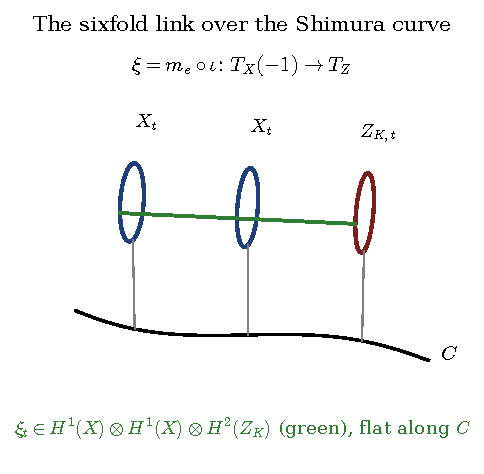
\includegraphics[width=0.78\textwidth]{figures/fig_link}
\caption{The sixfold link. Two copies of the Mumford fourfold $X_{t}$ and the sixfold $Z_{K,t}$ sit over the same point $t$ of the Shimura curve $C$; the class $\xi_{t}$ in the mixed K\"unneth component identifies the two copies of $T$ and is flat along $C$.}
\label{fig:link}
\end{figure*}

\begin{theorem}[The sixfold link]\label{thm:link}
Let $\xi$ be a nonzero element of $\Hom_{\Hdg}(T_{X}(-1),T_{Z})\subseteq H^{4}(X\times X\times Z_{K})$.
\begin{enumerate}[label=\textup{(\roman*)},leftmargin=2.4em,itemsep=2pt]
\item $\Hom_{\Hdg}(T_{X}(-1),T_{Z})=F\cdot\iota$ for the identification $\iota$ of Lemma~\ref{lem:tz}, so $\xi=m_{e}\circ\iota$ for a unique $e\in F^{\times}$. The $G\times K^{1}$-invariant classes of degree four on $X\times X\times Z_{K}$ have dimension $26$, and $\xi$ and $\psi\otimes\NS(Z_{K})$ are the only ones in the K\"unneth component $H^{1}(X)\otimes H^{1}(X)\otimes H^{2}(Z_{K})$.
\item If $\xi$ is algebraic, then $\xi^{\dagger}\xi$, the composite with the adjoint for the Lefschetz pairing on $X\times X$ and the intersection pairing on $Z_{K}$, is an algebraic endomorphism of $T_{X}(-1)$ equal to $m_{a(e)}$ with $a(e)=\kappa\,e^{2}c^{2}\in F$, $\kappa\in\QQ^{\times}$.
\item If $a(e)\notin\QQ$, the exceptional classes of $X\times X$ are algebraic at $t$, hence at every point of $C$, and so is every Hodge class on every power of $X$.
\item $a(e)\notin\QQ$ for every $e\in F^{\times}$ if and only if $K$ contains no imaginary quadratic field. If $K=F\cdot k$ with $k=\QQ(\sqrt{-d})$ and $c=f\sqrt{-d}$, then $a(e)\in\QQ$ exactly for $e\in\QQ f^{-1}$.
\item Conversely, if the exceptional classes are algebraic and some algebraic cycle on $X^{r}\times Z_{K}$ acts nonzero on $T_{Z}$, then every $\xi$ is algebraic.
\end{enumerate}
\end{theorem}

\begin{proof}
(i) Both sides are the irreducible $G$-representation $T$ with $\End_{\Hdg}=F$ \cite[Prop.~21.2]{BMB26}, so $\Hom_{\Hdg}=F\iota$. The count is the dimension of the kernel of the six raising and lowering operators of $\mathfrak{sl}_{2}^{3}$ on the torus-weight-zero part of $\bigwedge^{4}(V\oplus V\oplus D)$, computed by K\"unneth type: $(1,1,2)$ gives $3+3$, the line $F\iota$ and $\psi\otimes\NS(Z_{K})$; $(2,2,0)$ gives $4=\QQ\oplus F$, the Hodge classes of $X\times X$ in $H^{2}\otimes H^{2}$; $(0,0,4)$ gives $6=S^{2}\NS(Z_{K})$; $(2,0,2)$ and $(0,2,2)$ give $3$ each; and $(4,0,0)$, $(0,4,0)$, $(3,1,0)$, $(1,3,0)$ one each, products of divisor classes. The sum is $26$. The Hodge group of the product lies in $G\cdot K^{1}$, so $26$ bounds the Hodge classes from above; equality is not needed.

(ii) The adjoint of a correspondence for the Lefschetz pairing on $H^{2}(X\times X)$ and the polarised intersection pairing on $Z_{K}$ is the transposed cycle composed with cup products with powers of the polarisations and the inverse Lefschetz isomorphism, which is algebraic on an abelian variety \cite[\S2]{Kle68}; so $\xi^{\dagger}\xi$ is algebraic. By Lemma~\ref{lem:tz}, $T_{X}(-1)$ carries $-4q_{1}$ and $T_{Z}$ carries a rational multiple of $q_{c^{2}}$, and for $\xi=m_{e}$, $q_{c^{2}}(m_{e}x,m_{e}y)=\Tr(c^{2}e^{2}\trd(xy))=q_{1}(c^{2}e^{2}x,y)$, so $\xi^{\dagger}\xi=\kappa\,m_{e^{2}c^{2}}$.

(iii) An irrational $a\in F$ generates the cubic field, so every $m_{b}$, $b\in F$, is a polynomial in $\xi^{\dagger}\xi$, algebraic on $T_{X}(-1)$. Compose with the product map $\mu\colon H^{2}(X\times X)\supseteq T_{X}(-1)\to H^{2}(X)$ and its adjoint, both built from $\psi$, the diagonal and $\theta$ and hence algebraic \cite[Lem.~21.3]{BMB26}: the composite $\mu\circ(m_{b}\otimes1)\circ\mu^{\dagger}$ acts on the primitive part $U$ of $H^{2}(X)$ by the element $\nu(\Tr b-b)/2$ of $F$, irrational when $b$ is. With the identity and the projector onto $\QQ\theta$ this generates $\QQ\times F=\End_{\Hdg}H^{2}(X)$, so by \cite[Prop.~21.2]{BMB26} the exceptional classes are algebraic. The class $\xi$ is flat along $C$ and so are the exceptional classes, so by Lemma~\ref{lem:dichotomy} algebraicity at one point of the curve $C$ gives it on a countable set or everywhere; and \cite[Cor.~20.30]{BMB26} shows that algebraicity at one point of $C$ gives it at every point, and then every Hodge class on every power of $X$ is algebraic \cite[Thm.~21.7]{BMB26}.

(iv) $a(e)=\kappa e^{2}f^{2}\delta$ is rational iff $e^{2}f^{2}\delta\in\QQ$. If $-\delta\notin\QQ^{\times}(F^{\times})^{2}$ then $\delta\notin\QQ^{\times}(F^{\times})^{2}$ and $e^{2}f^{2}\delta\in\QQ$ is impossible. If $-\delta=-dg^{2}$ with $d\in\QQ^{\times}$, $g\in F^{\times}$, then with $c=f\sqrt{-d}$ one gets $a(e)=\kappa e^{2}f^{2}d$, rational iff $(ef)^{2}\in\QQ$ iff $ef\in\QQ$, a cubic field having no irrational element with rational square. And $-\delta\in\QQ^{\times}(F^{\times})^{2}$ exactly when $K\supseteq\QQ(\sqrt{-d})$ for some $d$.

(v) By \cite[Thm.~21.7]{BMB26} the Hodge conjecture holds for all powers of $X$ once the exceptional classes are algebraic. A cycle on $X^{r}\times Z_{K}$ acting nonzero on the irreducible $T_{Z}$ carries it isomorphically onto a summand of $H^{2k}(X^{r})(k-1)$; projecting onto that summand and composing with an isomorphism to $T_{X}(-1)\subseteq H^{2}(X\times X)$, a Hodge class on $X^{r+2}$ and algebraic, gives an algebraic nonzero element of $\Hom_{\Hdg}(T_{Z},T_{X}(-1))=F$; composing with the algebraic $m_{a}$ gives every element of that line, and transposing gives every $\xi$.
\end{proof}

\begin{proposition}[Hyper-K\"ahler carriers give $\pm1$]\label{prop:hk}
Let $Y_{1},\dots,Y_{m}$ be projective hyper-K\"ahler varieties of K3$^{[n_{j}]}$ type whose transcendental spaces are Hodge isometric to $(T,r_{j}q_{\lambda_{j}})$, $r_{j}\in\QQ^{\times}$, $\lambda_{j}\in F$ totally positive. Every composite of rational Hodge isometries between them that returns to $Y_{j}$ acts on $T$ by $\pm1$, and every composite of Hodge similarities by an element of $\QQ$.
\end{proposition}

\begin{proof}
A Hodge isometry $(T,r_{j}q_{\lambda_{j}})\to(T,r_{k}q_{\lambda_{k}})$ is a Hodge endomorphism of $T$, hence $m_{a}$ for some $a\in F$, and it is an isometry iff $r_{j}\lambda_{j}=r_{k}\lambda_{k}a^{2}$. A composite returning to $j$ is $m_{a}$ with $a^{2}=1$, and a composite of similarities is $m_{a}$ with $a^{2}\in\QQ$, which in a cubic field forces $a\in\QQ$. The isometries are algebraic by \cite{Bus19,Mar24}, which is why the statement matters: they realise $m_{b}$ between $S_{\lambda}$ and $S_{\lambda b^{-2}}$ and between their moduli spaces of sheaves, but every return is trivial.
\end{proof}

\subsection{Where the link stops}\label{ssec:f2stop2}

Theorem~\ref{thm:link} replaces the Kuga--Satake variety of \cite[Thm.~21.4]{BMB26}, of dimension $2^{7}$, by an abelian sixfold over the same curve, and it replaces the irrationality that had to be extracted from anticommuting Clifford blocks by the arithmetic of $K$: for every $K$ that is not a compositum $F\cdot k$ every link closes the target. Its logical status is the same as the Kuga--Satake link: by (v) it is equivalent to the target together with one algebraic link, not a reduction to something smaller.

The missing step is the algebraicity of one class $\xi\in H^{4}(X\times X\times Z_{K})$. It is exceptional: its component in $V\otimes V$ is the nine-dimensional $T$, not a multiple of $\psi$, so it is not invariant under $\Sp(V)$ and not in the Lefschetz algebra of $X\times X\times Z_{K}$ (Lemma~\ref{lem:sp-invariance}); the theorems that prove the conjecture when the Hodge ring is generated by divisors do not apply, and no Weil class of $Z_{K}$ or of $X\times X$ is involved. At the points of complex multiplication of $C$ the class $\xi_{c}$ is a Hodge class on a CM abelian variety in a mixed K\"unneth component between $X_{c}\times X_{c}$ and $Z_{K,c}$ with $\Hom(X_{c},Z_{K,c})=0$, so it is not a pull-back from one factor nor a product of lower-degree Hodge classes, and the generation theorems for CM abelian varieties do not reach it either. Unlike the Kuga--Satake class, the link is therefore not known even at the countably many special points. This is the price of staying inside abelian varieties, and it is the exact statement that \Fii{} needs at its smallest instance.

\section{Where the earlier attempt fails}\label{sec:earlier}

The preprint \cite{BB26} of the two authors claimed the conjecture in full. We record here each point at which it fails, so that the present paper can be read as its replacement and not as a continuation. Numbers refer to that preprint.

\paragraph{The secant cycle (Definition 3, Lemma 4).} For an abelian $2n$-fold $A$ of Weil type the preprint takes $\Sigma=\mathrm{Sec}^{n}(A^{\vee})$, the closure of the union of the $(n-1)$-planes spanned by $n$ points of $A^{\vee}$ in a projective embedding, and the cycle $Z_{\Sigma}=\Sigma\cap A^{\vee}$, asserted to have codimension $n$. Every point of $A^{\vee}$ lies on such a plane, so $A^{\vee}\subseteq\Sigma$ and $Z_{\Sigma}=A^{\vee}$: the intersection is not proper. The sheaf $\mathcal{O}_{\Sigma}|_{A^{\vee}}$ is $\mathcal{O}_{A^{\vee}}$, whose Fourier--Mukai transform is the skyscraper sheaf at the origin shifted by $-2n$, with Chern character the class of a point. So $\ch_{k}=0$ for $1\le k<2n$, contrary to Lemma~4, and Proposition~2 has nothing to identify with a Weil class.

\paragraph{The polarisation (Definition 3).} The polarisation is taken principal, so $\chi(L)=1$ and the embedding is into $\PP^{0}$; the dimension count needs $\chi(L)=2n^{2}+2n$. A principal polarisation is never very ample.

\paragraph{The dimension of the Weil space (Proposition 1).} $\det_{K}H^{1}(A)$ is a two-dimensional $\QQ$-space of Hodge classes \cite{Weil77}, so at a very general point $\Hdg^{n}(A)=\QQ\eta^{n}\oplus W(A)$ has dimension three, not two.

\begin{figure*}[t]
\centering
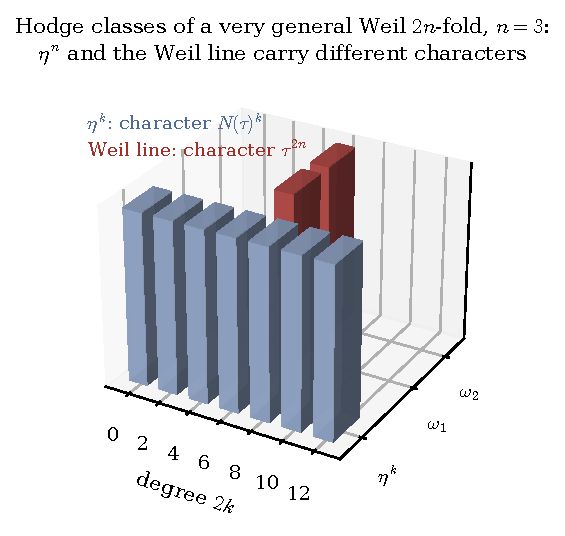
\includegraphics[width=0.92\textwidth]{figures/fig_eigen}
\caption{The Hodge classes of a very general abelian sixfold of Weil type and the characters of $K^{\times}$ on them: $\eta^{k}$ carries $N(\tau)^{k}$, the Weil plane carries $\tau^{2n}$. An eigenclass for $N^{n}$ in degree $2n$ is a multiple of $\eta^{n}$.}
\label{fig:eigen}
\end{figure*}

\paragraph{The eigencharacter (Lemmas 1, 2, Proposition 2, Theorem 4).} Equation~(1) of the preprint gives $\tau^{*}\eta=N(\tau)\eta$ for $\tau\in K^{\times}$, so $\eta^{n}$ has character $N(\tau)^{n}$, while Proposition~2 asserts character $1$. The group $K^{\times}$ acts on $W(A)=\bigwedge^{2n}_{K}H^{1}(A)$ by $\tau\mapsto\tau^{2n}$, which differs from $N(\tau)^{n}=(\tau\bar\tau)^{n}$ unless $(\tau/\bar\tau)^{n}=1$; so the Weil classes are not in the $N^{n}$-eigenspace, and an $N^{n}$-eigenclass of degree $2n$ is a multiple of $\eta^{n}$ (Fig.~\ref{fig:eigen}). The scaling of the secant sheaf by $d^{n}$ under an isogeny of degree $d$ (Lemma~1) is asserted without proof.

\paragraph{Step 4 of Theorem 4.} The points of a Shimura variety with smaller Mumford--Tate group are the points of proper special subvarieties, most of which are not of CM type; and Pohlmann's theorem \cite{Poh68} covers the CM types whose Hodge ring is generated by divisors, not all CM abelian varieties.

\paragraph{The reduction to Weil classes (Theorem 3, Section 5).} Moonen and Zarhin describe every Hodge class as a polynomial in divisor classes and Weil classes of isogeny factors in dimension at most five \cite{MZ99}, and the description is not known beyond; simple CM abelian varieties can carry Weil classes \cite{Weil77,Shi79b}; and not every factor of type IV is of Weil type.

\paragraph{Theorem 12.} The Kuga--Satake construction exists for Hodge structures of K3 type, with $h^{2,0}=1$ \cite{KS67,Del72}; Theorem~12 applies it to arbitrary primitive classes. Its algebraicity, credited there to Deligne, is open: Deligne proved that the correspondence is absolutely Hodge \cite{Del82}, and its algebraicity is known only in special families \cite{vG00,Var23}. Since the case split of Section~1.4 rests on this step for the classes of coniveau zero, it is incomplete.

None of these points is repaired here. The present paper does not use secant cycles, the eigencharacter argument or the Kuga--Satake construction outside K3 type, and it claims no case of the conjecture that is not proved in Sections~\ref{sec:reduction} to \ref{sec:f2}.

\begin{table*}[hbt!]
\centering
\caption{Every statement of the paper with its status. ``Proved'' means proved in the text from the cited results; ``open'' means not proved here or elsewhere to our knowledge.}
\label{tab:status}
\begin{ruledtabular}
\begin{tabular}{llll}
statement & where & status & what it needs \\
\colrule
$\HC\Leftrightarrow\Fii{}\wedge\Fiii{}$ & Thm.~\ref{thm:intro-reduction} & proved & -- \\
\Fii{} $\Leftrightarrow$ $\AB$ & Thm.~\ref{thm:f2isab} & proved & -- \\
six minimal sufficient sets & Prop.~\ref{prop:minimal} & proved, checked in Lean & -- \\
dichotomy of the algebraic locus & Lem.~\ref{lem:dichotomy} & proved & -- \\
\Fii{} as propagation from CM points & Thm.~\ref{thm:propagation} & proved & -- \\
Weil loci dense with CM base point & Prop.~\ref{prop:weil-dense} & proved in \cite{BMB26} & -- \\
chains make $e$ with $e^{2}\in\QQ$ algebraic & Thm.~\ref{thm:chain} & proved & a chain of the right multiplier \\
$\sqrt6$ algebraic on two-dimensional families & Thm.~\ref{thm:sqrt6} & proved & -- \\
$\sqrt5$, $\sqrt7$ algebraic on one-dimensional families & Thm.~\ref{thm:fricke} & proved & -- \\
similarities act by multipliers $d_{1}d_{2}$ & Prop.~\ref{prop:structure} & proved & -- \\
finite-group correspondences give abelian $E$ & Prop.~\ref{prop:hecke} & proved & -- \\
$\HC$ for $X\times X$, $X$ in the dihedral families & Cor.~\ref{cor:dihedral} & proved & -- \\
\Fiii{} for $S_{\lambda}$, $F=\QQ(\zeta_{7})^{+}$ or $\QQ(\zeta_{9})^{+}$, $D=D_{\infty}$ & Thm.~\ref{thm:zeta9} & proved & -- \\
where the dihedral mechanism stops & Prop.~\ref{prop:cubicstop} & proved & -- \\
\Fiii{} for $S_{\lambda}$, other cubic $F$ or other $D$ & Sect.~\ref{ssec:f3stop} & open & a non-similarity correspondence \\
\Fiii{} in general & -- & open & -- \\
product object of polarised shape & Thm.~\ref{thm:product} & proved & -- \\
direct sums never semiregular & Prop.~\ref{prop:directsum} & proved & -- \\
annihilator of the secant pieces is the product locus & Thm.~\ref{thm:annihilator} & proved & -- \\
secant and line-bundle pieces orthogonal & Prop.~\ref{prop:noorth} & false for every realisation & -- \\
(P2$'$) at a product point & Sect.~\ref{ssec:f2stop1} & open & $\Ext^{*}$ of secant sheaves \\
the Ext groups at the CM point $E_{0}^{6}$ & Lem.~\ref{lem:cmext} & proved & -- \\
no two-step cancellation of diagonal classes & Prop.~\ref{prop:twostep} & proved & -- \\
three line bundles at $E_{0}^{6}$ & Prop.~\ref{prop:separated} & proved, fail & -- \\
(P2$'$) at $E_{0}^{6}$, other configurations & Sect.~\ref{ssec:f2stop1} & open & the chain products \\
sixfold link $\Rightarrow$ exceptional classes & Thm.~\ref{thm:link} & proved & -- \\
algebraicity of the link $\xi$ & Sect.~\ref{ssec:f2stop2} & open & a cycle on $X\times X\times Z_{K}$ \\
dominant maps, blow-ups, derived equivalences preserve the defect & Prop.~\ref{prop:surgery} & proved & -- \\
exceptional classes of $X\times X$ & -- & open & -- \\
\Fii{} in general & -- & open & -- \\
the Hodge conjecture & -- & open & \Fii{} and \Fiii{} \\
\end{tabular}
\end{ruledtabular}
\end{table*}

\section{What is proved and what is open}\label{sec:status}


Table~\ref{tab:status} lists the statements. Three remarks on what the table says.

The two open statements are not independent problems that happen to add up to the conjecture; they are two halves of one phenomenon. Both say that the algebraic locus of a flat Hodge class, a countable union of closed strata through a dense set of points of complex multiplication, is not meagre. For \Fii{} the dense set is supplied by explicit cycles at CM points and the first instance is a single class on an abelian fourteenfold or a single Ext group on an eightfold; for \Fiii{} the dense set is supplied by the K3 surfaces with complex multiplication and by the chains of Section~\ref{sec:f3prime}, and the first instance is a cubic real multiplication on one K3 surface of Picard number $13$.

Each construction of this paper ends at a question with a definite answer. Whether some convolution of the pieces of Theorem~\ref{thm:product} has $\dim\Ext^{2}=57$ is a finite computation in the Ext algebra of two sheaves on a fourfold. Whether the link $\xi$ is algebraic is a question about one Hodge class on one abelian variety, equivalent by Theorem~\ref{thm:link}(v) to the exceptional classes together with one more cycle. Whether a correspondence acting on $T(S_{\lambda})$ otherwise than by a similarity exists is a question about one K3 surface. A negative answer to the first closes that route, as the analogous question on $E_{0}^{6}$ closed; a positive answer to any of them proves the corresponding statement at its first instance.

\subsection{Specialisation, degeneration and blow-ups}\label{ssec:bypass}

Three devices are often proposed for passing from the members where a class is known to be algebraic to the others, and it is worth recording exactly what each one proves.

\begin{proposition}\label{prop:bypass}
Let $\pi:\mathcal{X}\to B$ be a smooth projective family over an irreducible base and $\xi$ a flat Hodge class on its fibres.
\begin{enumerate}[label=\textup{(\roman*)},leftmargin=2.4em,itemsep=2pt]
\item If $\xi_{t}$ is algebraic at the generic point of a curve $C\subseteq B$ then it is algebraic at every point of $C$. The converse implication, from one point of $C$ to its generic point, holds when $\xi_{t_{0}}$ is the Chern character of a perfect complex whose semiregularity map is injective, and in no greater generality is it known.
\item Let $\tilde X$ be the blow-up of a smooth projective variety $X$ along a smooth closed subvariety $Z$ of codimension $c$. Then $\Hdg^{k}(\tilde X)/\Alg^{k}(\tilde X)\cong\Hdg^{k}(X)/\Alg^{k}(X)\oplus\bigoplus_{i=1}^{c-1}\Hdg^{k-i}(Z)/\Alg^{k-i}(Z)$. In particular the Hodge conjecture for $\tilde X$ is equivalent to the Hodge conjecture for $X$ and for $Z$, and no sequence of blow-ups and blow-downs reduces the defect of a variety.
\item For the Weil classes of $\cD_{n,n}$ and the exceptional class of a Mumford fourfold, every degeneration to a fibre with a semistable model on which the limit class is algebraic has its lift to the generic fibre as its missing step, and for the Mumford fourfold no degeneration keeping the class of Hodge type exists, since the Hodge locus of the class is a compact Shimura curve.
\end{enumerate}
\end{proposition}

\begin{proof}
(i) Specialisation of cycles along a curve \cite[Ch.~20]{Ful98} sends an algebraic cycle on the generic fibre to one on each special fibre with the same flat cohomology class; this is the direction used by Schoen's degeneration and by Proposition~\ref{prop:weil-dense}. In the other direction the algebraic locus is a countable union of closed sets by Lemma~\ref{lem:dichotomy}, and a point in one stratum says nothing about the stratum being the whole base; the one proved lift is the semiregularity theorem of Bloch, Buchweitz and Flenner \cite{Blo72,BF03}, which is the content of Theorem~\ref{thm:criterion}. (ii) Manin's decomposition of the motive of a blow-up \cite{Man68}, $h(\tilde X)=h(X)\oplus\bigoplus_{i=1}^{c-1}h(Z)(-i)$, is realised by the algebraic correspondences $\pi^{*}$ and $j_{*}\circ p^{*}\circ(\text{powers of the relative hyperplane class})$, which are compatible with Hodge classes and with algebraic classes; so both the Hodge classes and the algebraic classes of $\tilde X$ decompose accordingly, and the quotients add. A birational map between smooth projective varieties factors through blow-ups and blow-downs along smooth centres only in special cases, but every birational map is dominated by a sequence of blow-ups, and (ii) shows that the defect of the top variety is at least that of the bottom one, so the defect cannot be removed on the way. (iii) A flat class has a limit in the limit mixed Hodge structure of a semistable fibre, and on a totally degenerate fibre the graded pieces are combinatorial and every class is algebraic on the components; the return to the generic fibre is the lift of (i), with the same unproved step. For a Mumford fourfold the Hodge locus of the exceptional class is the compact Shimura curve of \cite[Thm.~21.7]{BMB26}, which has no boundary, so no fibre at which the class is still of Hodge type degenerates.
\end{proof}

The devices therefore relocate the two open statements without weakening them. The one true reduction in shape is Theorem~\ref{thm:propagation}: the whole of \Fii{} is equivalent to a lift from CM points along polarised abelian schemes, and the lift along each scheme is a question about one semiregular object at one point.

Nothing in the paper assumes an open statement, and no section depends on a computation that is not also proved by hand in the text. The machine checks of Appendix~\ref{app:checks} recompute the finite quantities; they do not carry any proof.


\appendix
\section{Machine checks}\label{app:checks}

Every finite quantity used in the proofs is recomputed by programs in the archive \cite{BB26code}, and the combinatorial and arithmetic statements among them are also proved in Lean~4. No statement of the paper rests on these checks; they guard against slips in the hand computations.

\paragraph{Lean.} The file \path{lean/HodgeClosure.lean} (Lean~4.24.0, no Mathlib) contains thirty-six theorems. Section~1 encodes the eight statements and the rule set of Table~\ref{tab:rules} as data, computes closures by iteration, and proves by evaluation that the closures of $\{\mathrm{F2},\mathrm{F3}'\}$, $\{\mathrm{F3}\}$, $\{\mathrm{L},\mathrm{M}\}$, $\{\mathrm{L},\mathrm{F3}'\}$ and $\{\mathrm{V},\mathrm{F3}'\}$ contain $\HC$, that the closures of $\{\mathrm{F2}\}$, $\{\mathrm{F3}'\}$, $\{\mathrm{L}\}$, $\{\mathrm{M}\}$, $\{\mathrm{V}\}$, $\{\AB\}$, $\{\mathrm{L},\mathrm{V}\}$ and $\{\mathrm{M},\mathrm{F3}'\}$ do not, and that the list of minimal sufficient sets, computed from the rule set alone, has exactly six members, those of Proposition~\ref{prop:minimal}. Section~2 works in $\ZZ[\sqrt{-d}]$ and proves that the hermitian form $\eta$ transforms under $\tau$ by $N(\tau)$, that the norm is multiplicative, that $\eta$ is not $K^{\times}$-invariant, and that the characters $N(\tau)^{n}$ and $\tau^{2n}$ differ at explicit $\tau$ (Section~\ref{sec:earlier}). Section~3 proves the dimension counts of Section~\ref{sec:f2}: $3n<n^{2}$ for $n\ge4$, $m^{2}+m'^{2}<(m+m')^{2}$ for $m,m'\ge1$ with $2mm'$ mixed directions, the values $r=57$ and $104$ of the lower bound, and the Hodge class count $26$ of Theorem~\ref{thm:link}(i) as a sum of K\"unneth contributions. Section~4 proves the polynomial identities behind the Fricke families of Section~\ref{ssec:fricke}: $c_{4}^{3}-c_{6}^{2}=1728\,t\,(t^{2}+13t+49)^{2}$ at level $7$ and $1728\,t\,(t^{2}+22t+125)^{3}$ at level $5$, by exact arithmetic on coefficient lists, together with the root products $7^{2}$ and $5^{3}$, the Euler numbers $12$ and $24$, the Shioda--Tate counts giving Picard number at least $16$, the transcendental rank $6$, and the dimensions $(n+1)/2$ of the dihedral Hecke algebras. Every theorem is checked by \texttt{\#print\,axioms}: thirty-four use no axiom, and the two inequalities proved with the arithmetic tactic use \texttt{propext} and \texttt{Quot.sound}.

The Lean certificate of \cite{BMB26}, \texttt{HodgeObstruction.lean} (Lean~4.34.0, \leancount{} theorems, each axiom-free or depending on \texttt{propext} only), carries the finite computations of that paper; it is cited and not repeated here. The reduction of Section~\ref{sec:reduction} uses only the hand-proved parts of \cite{BMB26}.

\paragraph{Python.} \path{code/sqrt6_chain.py} (sympy) implements Hilbert symbols and Hasse invariants exactly, verifies the product formula on random pairs, classifies $U_{\QQ}$, $E_{8}(-1)_{\QQ}$ and the invariant lattices, reproduces Varesco's embedding results for $\sqrt2$ and $\sqrt3$ as controls, searches the $165$ sign-admissible small forms $q_{E}$ over $\QQ(\sqrt6)$ ($98$ embed in $V_{3}$, $67$ do not), exhibits the complements $\langle1,-10\rangle$ and $\langle1,-1,-1,-1,-3,-30\rangle$, and checks both orders of the chain: twenty-five checks. \path{code/fricke_families.py} computes the fibre types, Euler numbers and Picard bounds of the Fricke curves and their twists at levels $5$ and $7$, checks numerically that the roots of $j(t)=j(\tau)$ are carried by $t\mapsto N^{k}/t$ to the $j$-invariants of the $N$-isogenous curves, verifies the twist identity $u_{p,q}(w(t))=pq\,u_{w(p),w(q)}(t)/t^{2}$, the M\"obius transformations preserving the labelled points, the embedding of every rank-six form of signature $(2,4)$ in $V_{2}$ and $V_{3}$ after any scaling, and the Hecke algebras of $(D_{n},\langle\tau\rangle)$ for $n=5,7,9,11$: forty-one checks. \path{code/product_object.py} builds the exterior-algebra model of $H^{*}(A\times A')$ for $(m,m')=(2,1),(2,2)$, the tangent space of $\cD_{n,n}$ and of the product locus, the first-order Hodge loci of the exterior products and of the object of Theorem~\ref{thm:product}, the Vandermonde determinant, the vanishing of the cross terms, and the Hankel rank and $r(\gamma)$ of the final class; \path{code/convolution_checks.py} computes in the same model the rank of $v\mapsto v\lrcorner\theta_{A}$ on $T\cD_{n,n}$, the contraction ranks of $\ch(\mathcal{E}')$ and $\ch(\mathcal{E}'')$ in Proposition~\ref{prop:convolution}(iii), and the trace of an upper triangular times a strictly upper triangular block matrix. In these two programs ranks are computed in floating point with a relative tolerance of $10^{-7}$ and agree with the closed formulas. \path{code/sixfold_link.py} checks the alternation and invariances of $\psi_{c}$, the decomposition of the $K^{1}$-invariants, the ratio of the induced forms at the three places, the symmetry of $T_{X}(-1)$, the count $26$ and the weight support of $\xi$; \path{code/link_weights.py} computes the Hodge classes of degree four on $X\times X\times Z_{K}$ under the three groups of Section~\ref{ssec:f2stop2} and the vanishing of $\Hom(X_{c},Z_{K,c})$ at the compositum CM point. \path{code/closure_graph.py} recomputes the closures and the minimal sets, and \path{code/bypass_checks.py} the Horn closure with the facts of the literature on abelian varieties adjoined and the blow-up bookkeeping of Proposition~\ref{prop:bypass}(ii).

\paragraph{Julia, C, C\texttt{++} and shell.} \path{code/closure_graph.jl}, \path{code/closure_graph.c} and \path{code/closure_graph.cpp} recompute the closures of all $256$ subsets of the eight statements and the six minimal sets by three independent implementations of the fixed-point iteration; \path{code/eigencharacter.jl} recomputes the characters of Section~\ref{sec:earlier} in exact integer arithmetic, and \path{code/hilbert.c} the Hilbert symbols and the invariants of Table~\ref{tab:invariants}; \path{code/run_all.sh} runs every program and the Lean file and prints a line per check. The expected outputs are recorded in \path{code/EXPECTED.md}.


\section*{Acknowledgements}
The paper builds on the theorems of Eyal Markman on secant sheaves and Weil classes, on the work of Bert van Geemen, Matthias Sch\"utt and Mauro Varesco on real multiplication of K3 surfaces, on Nikolay Buskin's theorem on Hodge isometries, on the semiregularity theory of Spencer Bloch, Ragnar-Olaf Buchweitz and Hubert Flenner, and on the descriptions of Hodge classes on abelian varieties by Ben Moonen, Yuri Zarhin, Yves Andr\'e and James Milne. We thank Priyabrata Mandal for the collaboration on the earlier paper \cite{BMB26} whose results are used here.

\section*{Data and code availability}
The \LaTeX{} source of the paper, the Python, Julia, C, C\texttt{++} and shell programs of Appendix~\ref{app:checks} and the Lean~4 file are archived at Zenodo, release v2.7.0, under the concept DOI \href{https://doi.org/\zenodoCodeID}{\nolinkurl{doi:\zenodoCodeID}} of all versions \cite{BB26code}; the compiled paper is the only file of the folder \texttt{preprints} of that archive. The candidate configurations of Section~\ref{ssec:e06count} and the first enumerations of their chains, among them that of Remark~\ref{rem:sevenbundles}, were produced with Anaxia, the construction engine of the BLLM project \cite{Bha26bllm}, release v3.0.5, archived at Zenodo under \href{https://doi.org/10.5281/zenodo.23469389}{\nolinkurl{doi:10.5281/zenodo.23469389}}, and the support results of Section~\ref{ssec:supports} with release v3.1.0 \cite{Bha26bllmb}, archived under \href{https://doi.org/10.5281/zenodo.23484160}{\nolinkurl{doi:10.5281/zenodo.23484160}}; the point counts of Remark~\ref{rem:frickepicard} follow the Frobenius test of its module \texttt{k3frob} (commit \texttt{8782bd3}), which first showed that a Fricke self-map is a complex and not a real multiplication, at level $13$; every statement of the paper is decided by the proofs in the text and by the programs of the archive, not by the engine. Deep Bhattacharjee carried out the constructions on \Fii{} and \Fiii{} and the Lean, Julia, C, C\texttt{++}, Python and shell verifications with the help of AI assistance (Claude, Anthropic). Both authors approved the final version.

\section*{Ethical declarations}
Funding: none. Competing interests: none.


\begin{thebibliography}{99}\raggedright

\bibitem{And92}
Y. Andr\'e,
\emph{Mumford--Tate groups of mixed Hodge structures and the theorem of the
fixed part},
Compositio Math. \textbf{82} (1992), no.~1, 1--24.
\href{http://www.numdam.org/item/CM_1992__82_1_1_0/}{\nolinkurl{numdam.org/item/CM_1992__82_1_1_0}}.

\bibitem{And96b}
Y. Andr\'e,
\emph{Pour une th\'eorie inconditionnelle des motifs},
Inst. Hautes \'Etudes Sci. Publ. Math. \textbf{83} (1996), 5--49.
\href{https://doi.org/10.1007/BF02698643}{\nolinkurl{doi:10.1007/BF02698643}}.

\bibitem{BB26}
D. Bhattacharjee and U. Bhattacharya,
\emph{Relative secant cycles and Hodge classes},
Preprints.org, version 5, 2026.
\href{https://doi.org/10.20944/preprints202602.0462.v5}{\nolinkurl{doi:10.20944/preprints202602.0462.v5}}.

\bibitem{BB26code}
D. Bhattacharjee and U. Bhattacharya,
\emph{Source and verification code for the paper ``Algebraic Loci of Hodge Classes and the Two Statements Left on Abelian Varieties''},
Zenodo, 2026.
\href{https://doi.org/\zenodoCodeID}{\nolinkurl{doi:\zenodoCodeID}}.

\bibitem{BF03}
R.-O. Buchweitz and H. Flenner,
\emph{A semiregularity map for modules and applications to deformations},
Compositio Math. \textbf{137} (2003), no.~2, 135--210.
\href{https://doi.org/10.1023/A:1023999012081}{\nolinkurl{doi:10.1023/A:1023999012081}}.

\bibitem{Blo72}
S. Bloch,
\emph{Semi-regularity and de Rham cohomology},
Invent. Math. \textbf{17} (1972), 51--66.
\href{https://doi.org/10.1007/BF01390023}{\nolinkurl{doi:10.1007/BF01390023}}.

\bibitem{BMB26}
D. Bhattacharjee, P. Mandal and U. Bhattacharya,
\emph{Algebraic loci of Weil classes on abelian varieties},
preprint, 2026, with its source and verification archive, Zenodo, release v5.0.1.
\href{https://doi.org/10.5281/zenodo.23225483}{\nolinkurl{doi:10.5281/zenodo.23225483}}.

\bibitem{Bus19}
N. Buskin,
\emph{Every rational Hodge isometry between two K3 surfaces is algebraic},
J. Reine Angew. Math. \textbf{755} (2019), 127--150.
\href{https://doi.org/10.1515/crelle-2017-0027}{\nolinkurl{doi:10.1515/crelle-2017-0027}}.

\bibitem{BvGS24}
E. Bayer-Fluckiger, B. van Geemen and M. Sch\"utt,
\emph{K3 surfaces with real or complex multiplication},
preprint, 2024.
\href{https://arxiv.org/abs/2401.04072}{\nolinkurl{arXiv:2401.04072}}.

\bibitem{dCM02}
M. A. de Cataldo and L. Migliorini,
\emph{The Chow groups and the motive of the Hilbert scheme of points on a
surface},
J. Algebra \textbf{251} (2002), no.~2, 824--848.
\href{https://doi.org/10.1006/jabr.2001.9105}{\nolinkurl{doi:10.1006/jabr.2001.9105}}.

\bibitem{Del71}
P. Deligne,
\emph{Th\'eorie de Hodge. II},
Inst. Hautes \'Etudes Sci. Publ. Math. \textbf{40} (1971), 5--57.
\href{https://doi.org/10.1007/BF02684692}{\nolinkurl{doi:10.1007/BF02684692}}.

\bibitem{Del72}
P. Deligne,
\emph{La conjecture de Weil pour les surfaces $K3$},
Invent. Math. \textbf{15} (1972), 206--226.
\href{https://doi.org/10.1007/BF01404126}{\nolinkurl{doi:10.1007/BF01404126}}.

\bibitem{Del82}
P. Deligne,
\emph{Hodge cycles on abelian varieties} (notes by J. S. Milne),
in: Hodge Cycles, Motives, and Shimura Varieties,
Lecture Notes in Math. \textbf{900}, Springer, Berlin, 1982, pp.~9--100.
\href{https://doi.org/10.1007/978-3-540-38955-2_3}{\nolinkurl{doi:10.1007/978-3-540-38955-2_3}}.

\bibitem{Ful98}
W. Fulton,
\emph{Intersection Theory}, 2nd ed.,
Ergebnisse der Mathematik und ihrer Grenzgebiete (3) \textbf{2},
Springer, New York, 1998.
\href{https://doi.org/10.1007/978-1-4612-1700-8}{\nolinkurl{doi:10.1007/978-1-4612-1700-8}}.

\bibitem{Gro61}
A. Grothendieck,
\emph{Techniques de construction et th\'eor\`emes d'existence en g\'eom\'etrie
alg\'ebrique IV: les sch\'emas de Hilbert},
S\'eminaire Bourbaki, Vol.~6 (1960/61), Exp. No.~221, 249--276;
reprinted by Soc. Math. France, Paris, 1995.

\bibitem{GS07}
A. Garbagnati and A. Sarti,
\emph{Symplectic automorphisms of prime order on K3 surfaces},
J. Algebra \textbf{318} (2007), no.~1, 323--350.
\href{https://doi.org/10.1016/j.jalgebra.2007.04.017}{\nolinkurl{doi:10.1016/j.jalgebra.2007.04.017}}.

\bibitem{GW09}
R. Goodman and N. R. Wallach,
\emph{Symmetry, Representations, and Invariants},
Graduate Texts in Mathematics \textbf{255}, Springer, New York, 2009.
\href{https://doi.org/10.1007/978-0-387-79852-3}{\nolinkurl{doi:10.1007/978-0-387-79852-3}}.

\bibitem{Hod50}
W. V. D. Hodge,
\emph{The topological invariants of algebraic varieties},
in: Proceedings of the International Congress of Mathematicians (Cambridge, Mass., 1950), Vol.~1,
Amer. Math. Soc., Providence, 1952, pp.~182--192.

\bibitem{Huy19}
D. Huybrechts,
\emph{Motives of isogenous K3 surfaces},
Comment. Math. Helv. \textbf{94} (2019), no.~3, 445--458.
\href{https://doi.org/10.4171/CMH/465}{\nolinkurl{doi:10.4171/CMH/465}}.

\bibitem{Kle68}
S. L. Kleiman,
\emph{Algebraic cycles and the Weil conjectures},
in: Dix expos\'es sur la cohomologie des sch\'emas,
North-Holland, Amsterdam, 1968, pp.~359--386.

\bibitem{KS67}
M. Kuga and I. Satake,
\emph{Abelian varieties attached to polarized $K3$-surfaces},
Math. Ann. \textbf{169} (1967), 239--242.
\href{https://doi.org/10.1007/BF01399540}{\nolinkurl{doi:10.1007/BF01399540}}.

\bibitem{Lef24}
S. Lefschetz,
\emph{L'analysis situs et la g\'eom\'etrie alg\'ebrique},
Gauthier-Villars, Paris, 1924.

\bibitem{Man68}
Ju. I. Manin,
\emph{Correspondences, motifs and monoidal transformations},
Math. USSR-Sb. \textbf{6} (1968), no.~4, 439--470.
\href{https://doi.org/10.1070/SM1968v006n04ABEH001070}{\nolinkurl{doi:10.1070/SM1968v006n04ABEH001070}}.

\bibitem{Mar24}
E. Markman,
\emph{Rational Hodge isometries of hyper-K\"ahler varieties of K3$^{[n]}$
type are algebraic},
Compos. Math. \textbf{160} (2024), no.~6, 1261--1303.
\href{https://doi.org/10.1112/S0010437X24007048}{\nolinkurl{doi:10.1112/S0010437X24007048}}.

\bibitem{Mar25a}
E. Markman,
\emph{Cycles on abelian $2n$-folds of Weil type from secant sheaves on abelian
$n$-folds}, preprint, arXiv:2502.03415 (2025).
\href{https://doi.org/10.48550/arXiv.2502.03415}{\nolinkurl{doi:10.48550/arXiv.2502.03415}}.

\bibitem{Mar25b}
E. Markman,
\emph{Secant sheaves and Weil classes on abelian varieties},
preprint, arXiv:2509.23403 (2025).
\href{https://doi.org/10.48550/arXiv.2509.23403}{\nolinkurl{doi:10.48550/arXiv.2509.23403}}.

\bibitem{Mar25c}
E. Markman,
\emph{Secant sheaves on abelian $n$-folds with real multiplication and Weil
classes on abelian $2n$-folds with complex multiplication},
preprint, 2025.
\href{https://arxiv.org/abs/2509.23079}{\nolinkurl{arXiv:2509.23079}}.

\bibitem{Mil20}
J. S. Milne,
\emph{Hodge classes on abelian varieties},
preprint, 2020.
\href{https://arxiv.org/abs/2010.08857}{\nolinkurl{arXiv:2010.08857}}.

\bibitem{Mor84}
D. R. Morrison,
\emph{On K3 surfaces with large Picard number},
Invent. Math. \textbf{75} (1984), no.~1, 105--121.
\href{https://doi.org/10.1007/BF01403093}{\nolinkurl{doi:10.1007/BF01403093}}.

\bibitem{Mum69}
D. Mumford,
\emph{A note of Shimura's paper ``Discontinuous groups and abelian
varieties''},
Math. Ann. \textbf{181} (1969), 345--351.
\href{https://doi.org/10.1007/BF01350672}{\nolinkurl{doi:10.1007/BF01350672}}.

\bibitem{MZ95}
B. Moonen and Yu. G. Zarhin,
\emph{Hodge classes and Tate classes on simple abelian fourfolds},
Duke Math. J. \textbf{77} (1995), no.~3, 553--581.
\href{https://doi.org/10.1215/S0012-7094-95-07717-5}{\nolinkurl{doi:10.1215/S0012-7094-95-07717-5}}.

\bibitem{MZ99}
B. Moonen and Yu. G. Zarhin,
\emph{Hodge classes on abelian varieties of low dimension},
Math. Ann. \textbf{315} (1999), no.~4, 711--733.
\href{https://doi.org/10.1007/s002080050333}{\nolinkurl{doi:10.1007/s002080050333}}.

\bibitem{Nik80}
V. V. Nikulin,
\emph{Integral symmetric bilinear forms and some of their applications},
Math. USSR Izv. \textbf{14} (1980), no.~1, 103--167.
\href{https://doi.org/10.1070/IM1980v014n01ABEH001060}{\nolinkurl{doi:10.1070/IM1980v014n01ABEH001060}}.

\bibitem{Poh68}
H. Pohlmann,
\emph{Algebraic cycles on abelian varieties of complex multiplication type},
Ann. of Math. (2) \textbf{88} (1968), 161--180.
\href{https://doi.org/10.2307/1970570}{\nolinkurl{doi:10.2307/1970570}}.

\bibitem{Pri24}
J. P. Pridham,
\emph{Semiregularity as a consequence of Goodwillie's theorem},
Forum Math. Sigma \textbf{12} (2024), e126. arXiv:1208.3111.
\href{https://doi.org/10.1017/fms.2024.132}{\nolinkurl{doi:10.1017/fms.2024.132}}.

\bibitem{Ser73}
J.-P. Serre,
\emph{A Course in Arithmetic},
Graduate Texts in Mathematics \textbf{7}, Springer, New York, 1973.
\href{https://doi.org/10.1007/978-1-4684-9884-4}{\nolinkurl{doi:10.1007/978-1-4684-9884-4}}.

\bibitem{Shi63}
G. Shimura,
\emph{On analytic families of polarized abelian varieties and automorphic functions},
Ann. of Math. (2) \textbf{78} (1963), 149--192.
\href{https://doi.org/10.2307/1970507}{\nolinkurl{doi:10.2307/1970507}}.

\bibitem{Shi79b}
T. Shioda,
\emph{The Hodge conjecture for Fermat varieties},
Math. Ann. \textbf{245} (1979), 175--184.
\href{https://doi.org/10.1007/BF01428804}{\nolinkurl{doi:10.1007/BF01428804}}.

\bibitem{Ste85}
H. Sterk,
\emph{Finiteness results for algebraic K3 surfaces},
Math. Z. \textbf{189} (1985), no.~4, 507--513.
\href{https://doi.org/10.1007/BF01168156}{\nolinkurl{doi:10.1007/BF01168156}}.

\bibitem{Var23}
M. Varesco,
\emph{Hodge similarities, algebraic classes, and Kuga--Satake varieties},
Math. Z. \textbf{305} (2023), paper no.~69.
\href{https://doi.org/10.1007/s00209-023-03390-8}{\nolinkurl{doi:10.1007/s00209-023-03390-8}}.

\bibitem{vG00}
B. van Geemen,
\emph{Kuga--Satake varieties and the Hodge conjecture},
in: The Arithmetic and Geometry of Algebraic Cycles (Banff, 1998),
NATO Sci. Ser. C Math. Phys. Sci. \textbf{548},
Kluwer, Dordrecht, 2000, pp.~51--82.
\href{https://doi.org/10.1007/978-94-011-4098-0_3}{\nolinkurl{doi:10.1007/978-94-011-4098-0_3}}.

\bibitem{vG08}
B. van Geemen,
\emph{Real multiplication on K3 surfaces and Kuga--Satake varieties},
Michigan Math. J. \textbf{56} (2008), no.~2, 375--399.
\href{https://doi.org/10.1307/mmj/1224783519}{\nolinkurl{doi:10.1307/mmj/1224783519}}.

\bibitem{vGS07}
B. van Geemen and A. Sarti,
\emph{Nikulin involutions on K3 surfaces},
Math. Z. \textbf{255} (2007), no.~4, 731--753.
\href{https://doi.org/10.1007/s00209-006-0047-6}{\nolinkurl{doi:10.1007/s00209-006-0047-6}}.

\bibitem{vGS25}
B. van Geemen and M. Sch\"utt,
\emph{On families of K3 surfaces with real multiplication},
Forum Math. Sigma \textbf{13} (2025), Paper No. e2.
\href{https://doi.org/10.1017/fms.2024.146}{\nolinkurl{doi:10.1017/fms.2024.146}}.

\bibitem{Weil77}
A. Weil,
\emph{Abelian varieties and the Hodge ring},
in: \OE uvres Scientifiques, Collected Papers, Vol.~III,
Springer, New York, 1979, pp.~421--429.

\bibitem{Zar83}
Yu. G. Zarhin,
\emph{Hodge groups of K3 surfaces},
J. Reine Angew. Math. \textbf{341} (1983), 193--220.
\href{https://doi.org/10.1515/crll.1983.341.193}{\nolinkurl{doi:10.1515/crll.1983.341.193}}.

\end{thebibliography}


\end{document}
